% !TEX root = ../thesis.tex


\chapter{Tests and Results}
% \label{cha:eva_tests_results}

In this chapter I will first present a few benchmarks. It is important for any simulation to be able to reproduce results that are predicted by theory. For this, I will test collision rates depending on temperature and scattering length as well as the relaxation of the cloud from an initial delta velocity distribution to a Maxwell-Boltzmann distribution. 

Then I am going to show how our proposed solution of a compressing box potential compares to similar setups with harmonic trapping configurations in terms of evaporation efficiency and final atom numbers.


\section{Benchmarks}

\subsection{Collision Rates}
% Our first test is if the simulation can reproduce accurate collision rates that match the theoretical predictions. For the cross section given in \cref{eq:crosssection}, we have to take the average \meanProb over the Maxwell-Boltzmann distributions for both collision partners to find the mean collision rate.
% \begin{align*}
%     \meanProb &= \iint \multidiff{3}{c_1} \multidiff{3}{c_2}\; \frac{8\pi a^2\crel}{1 + a^2 k^2} \times n(\vec{c}_1) n(\vec{c}_2) \\
%     &= \frac{8\pi a^2}{(2\pi m \kB T)^3}\iint \multidiff{3}{c_1} \multidiff{3}{c_2}\; \frac{\crel}{1 + a^2 k^2} \exp\!\left(-\frac{m(\vec{c}_1^2 + \vec{c}_2^2)}{2\kB T}\right) 
%     \intertext{We can now change variables to centre-of-mass and relative coordinates and integrate out the angular part}
%     &= (4\pi)^2 \frac{8\pi a^2}{(2\pi m \kB T)^3}\int_0^\infty \diff{\crel}\; \crel^2 \frac{\crel}{1 + a^2 k^2} \exp\!\left(-\frac{m\crel^2}{4\kB T}\right) \nonumber \\
%     &\phantom{=} \quad \times \int_0^\infty \diff{c_\text{COM}}\; c_\text{COM}^2 \exp\!\left(-\frac{mc_\text{COM}^2}{\kB T}\right) \\
%     &= 4\sqrt{\pi} a^2 \left(\frac{m}{\kB T}\right)^\frac{3}{2} \int_0^\infty \diff{\crel} \frac{\crel^2}{1 + a^2 \frac{m^2 \crel^2}{4\hbar^2}} \exp\!\left(-\frac{m\crel^2}{4\kB T}\right)
%     \intertext{where we have performed the integration over $c_\text{COM}$ and used the relation $k = \frac{m\crel}{2\hbar}$. Making the integral dimensionless and introducing the (also dimensionless) parameter $\chi = \sqrt{\frac{\hbar^2}{a^2 m \kB T}}$ we find}
%     &= 64\sqrt{\pi} \cdot \frac{a\hbar}{m} \cdot \chi \int_0^\infty \diff{u}\; \frac{u^3}{\chi^2 + u^2} \exp(-u^2) \\
%     &= 32\sqrt{\pi} \cdot \frac{a\hbar}{m} \cdot \chi \left(1 + \chi^2\exp(\chi^2)\text{Ei}(-\chi^2)\right)
%     \intertext{where Ei is the exponential integral \cite[Eq.~6.2.5]{NIST:DLMF}. Because $\chi^2$ can be much larger than 1, for calculation on a computer it is better to express this using the confluent hypergeometric function $U$ \cite[Eq.~13.2.6]{NIST:DLMF}:}
%     \meanProb &= 32\sqrt{\pi} \cdot \frac{a\hbar}{m} \cdot \chi \left(1 + \chi^2U(1,1,\chi^2)\right).
% \end{align*}
% We can now use our previous result for the mean spatial density in an arbitrary power-law trap from \cref{eq:spatial_density,eq:mean_density} to find the mean collision rate $\langle\Rcoll\rangle$ as
% \begin{align*}
%     \langle\Rcoll\rangle &= \langle n\rangle \meanProb \\
%     &= 4\sqrt{\pi} \frac{N}{x_0y_0z_0} \cdot \frac{a\hbar}{m} \cdot \chi \left(1 + \chi^2U(1,1,\chi^2)\right) \times \prod_{i\in\{x,y,z\}}\frac{1}{\Gamma\!\left(1 + \frac{1}{\alpha_i}\right)}\left(\frac{U_i}{2 \kB T}\right)^{\frac{1}{\alpha_i}}. 
% \end{align*}
Our first test is if the simulation can reproduce accurate collision rates that match the theoretical predictions. For the cross section given in \cref{eq:crosssection}, we have to take the average \meanProb over the Maxwell-Boltzmann distributions for both collision partners to find the mean collision rate. This calculation is done in \cref{sec:appendix_average} and the result is
\begin{equation*}
    \meanProb = 32\sqrt{\pi} \cdot \frac{a\hbar}{m} \cdot \chi \left(1 + \chi^2U(1,1,\chi^2)\right),
\end{equation*}
where
\begin{equation*}
    \chi = \sqrt{\frac{\hbar^2}{a^2 m \kB T}}
\end{equation*}
is a dimensionless parameter that combines the scattering length $a$, the atomic mass $m$ and the temperature $T$. $U(1,1,\chi^2)$ is one of the confluent hypergeometric functions \cite[Eq.~13.2.6]{NIST:DLMF}.

We can now use our previous result for the mean spatial density in an arbitrary power-law trap from \cref{eq:spatial_density,eq:mean_density} to find the mean collision rate $\langle\Rcoll\rangle$ as
\begin{equation}\label{eq:meancollisionrate}
    \langle\Rcoll\rangle = \langle n\rangle \meanProb = 4\sqrt{\pi} \frac{N}{x_0y_0z_0} \cdot \frac{a\hbar}{m} \cdot \chi \left(1 + \chi^2U(1,1,\chi^2)\right) \times \prod_{i\in\{x,y,z\}}\frac{1}{\Gamma\!\left(1 + \frac{1}{\alpha_i}\right)}\left(\frac{U_i}{2 \kB T}\right)^{\frac{1}{\alpha_i}}. 
\end{equation}

To validate the accuracy of the simulation, we test this for different scattering lengths and temperatures. We choose a (near) box potential with $\alpha_x = \alpha_y = \alpha_z = 1000$, side lengths of \SI{1}{mm} in all directions and a potential depth of $U_0 = \SI{e-26}{J} \sim \SI{725}{\micro\kelvin}\times\kB$. The atomic mass is set to \SI{87}{u}. We start each of the simulations with \num{4e8} atoms in a $(\num{0.995} \times \num{0.995} \times \num{0.995})\, \si{\milli\meter\cubed}$ cube with uniform density distribution, let them reach a steady state by waiting for 3 initial mean collision times and then let the simulation continue until 100 initial mean collision times have been elapsed.

The statistic weight is \num{32768}, meaning \num{12207} particles are simulated. The timestep is 1/50 of the mean collision time and for this test, the loss coefficients $K_{1,2,3}$ are all set to 0. The results are shown in \cref{fig:evap_test_rates} and the measured rates fit the prediction very well. Over all conducted tests, the maximum deviation of the measured from the theoretically predicted rate was \SI{.784}{\percent}, with an average of just \SI{.414}{\percent}.

\vfill
\begin{figure}[hbp]
    \centering
    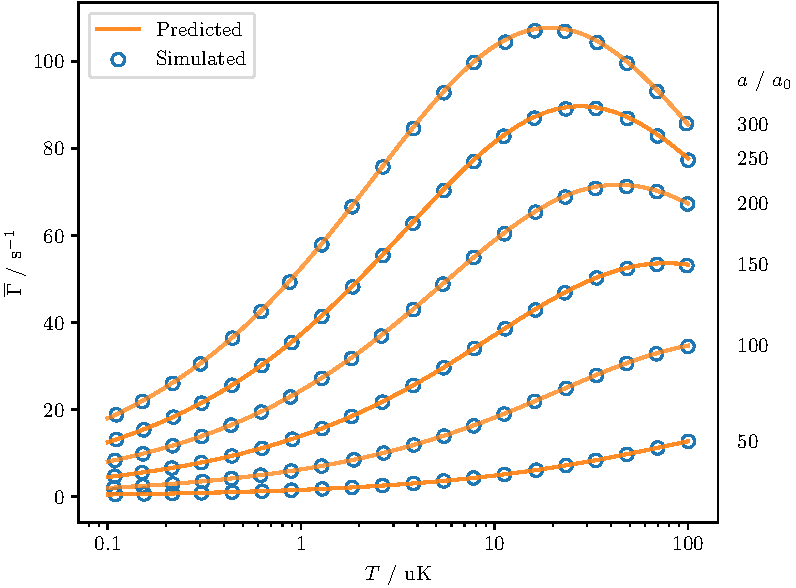
\includegraphics[]{Evap/CollisionRates}
    \caption[Collision rate variation with temperature and scattering length]{\num{4e8} atoms are simulated in an approximate box potential with a volume of $\sim\!\SI{1}{\milli\meter\cubed}$ at different values of the scattering length $a$ and temperature $T$. The collision time is averaged over 100 initial mean collision times and compared to the theoretical result from \cref{eq:meancollisionrate}. The maximum deviation was measured to be \SI{.784}{\percent}.}
    \label{fig:evap_test_rates}
\end{figure}
\vfill


\subsection{Thermal Relaxation}
Next, we initialise a cloud of \num{3e8} atoms in the same potential as before and with a scattering length of $a = 100\, a_0$. The kinetic temperature is set to $T=\SI{20}{\micro\kelvin}$, but every particle is given the same speed initially. We record the speeds of every particle present for 10 initial mean collision times ${\langle \tau\rangle}_\text{i}$ and average the resulting speed distribution over 50 separate runs. The results are shown in \cref{fig:evap_relaxation}. After $\num{8.5}\,{\langle \tau\rangle}_\text{i}$, the resulting speed distribution matches the expected Maxwell-Boltzmann distribution.
\begin{figure}[htbp]
    \centering
    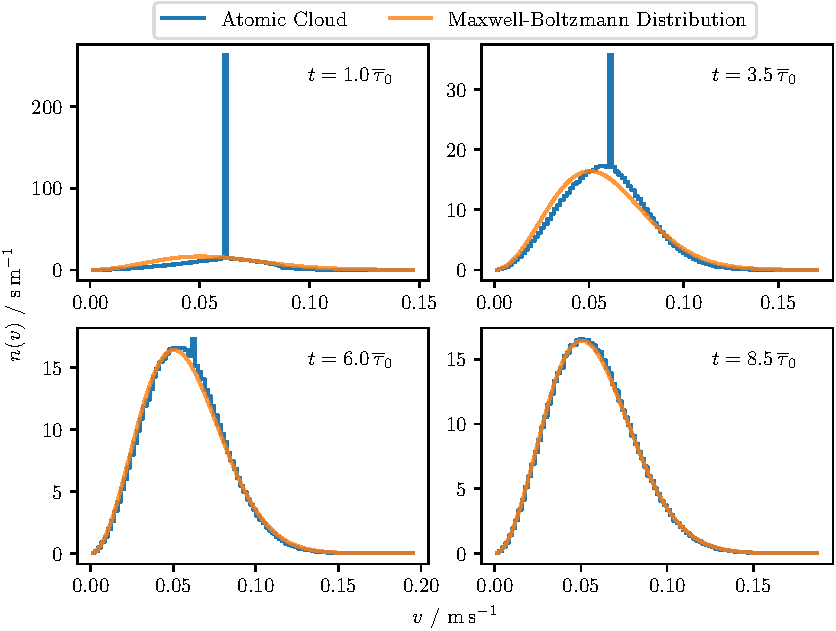
\includegraphics[]{Evap/Relaxation}
    \caption[Relaxation to a Maxwell-Boltzmann distribution]{The simulation is initialised with \num{3e8} atoms that all start with the same speed. Over a total of 10 initial mean collision times, the relaxation of the speeds to a Maxwell-Boltzmann distribution is observed.}
    \label{fig:evap_relaxation}
\end{figure}

% \subsection{Internal Energy per Atom}
% Our last test analyses the energy per particle. From the theoretical analysis, we expect \[\tilde{E} = \xi kB T, \quad \xi = \frac{3}{2} + \frac{1}{\alpha_x} + \frac{1}{\alpha_y} + \frac{1}{\alpha_z}\] per particle in a power-law potential with exponents $\alpha_{x,y,z}$.
% We let \[\alpha_x = \alpha_y = \alpha_z \equiv \alpha,\quad 1 \leq \alpha \leq 100.\] The starting conditions are: \todo[inline]{atom number, density, temperature} and we let the system reach equlibrium in \dots initial mean collision times, before we measure the energy per particle. The results of this can be seen in Figure~\todo{ref}. Again, we see excellent agreement with the theoretical prediction.


\section{Efficient Evaporation in a Box}
\label{sec:eva_test}
We now move on to test the proposed evaporation in a box potential. The simulation is partly based on the assumption that the atoms have been cooled to a high starting phase space density before the evaporation sequence. This goes hand in hand with our initial concept for evaporation in a box. Usually, atoms are pre-cooled before evaporative cooling in an optical dipole trap is carried out. It has been shown that $\Lambda$-enhanced grey molasses cooling is possible on the D2 line of $^{87}$Rb \cite{Rosi2018enhancedGM}. Here, a final phase space density of \num{4e-6} was achieved at a temperature of \SI{4}{\micro\kelvin}, corresponding to a density of \SI{4.9e9}{\per\centi\meter\cubed}. Starting from a density this low would be disadvantageous for evaporative cooling as it would incur high thermalisation times. Compressing the cloud however would heat the atoms again. Grey molasses cooling is mainly limited by time as the cloud can expand freely and is subject to gravity. With our proposed concept of a box potential, the cloud would not be able to expand indefinitely, given that the trap depth is high enough to contain the falling atoms. We could then repeatedly compress the gas and cool it again. Such an alternating cycle of compression and cooling has already been demonstrated with $^{85}$Rb using a near-resonant dark optical lattice, leading to a density of \SI{1.2e12}{\per\centi\meter\cubed} with a temperature of \SI{10}{\micro\kelvin}, equivalent to a phase space density of \num{2.6e-4} \cite{PhysRevA.72.043410}. 

For the simulation, we use a box potential created from two ring beams that intersect each other at an angle. The functional form of this potential is
\begin{equation} \label{eq:eva_potential}
    U(\vec{r}) = U_0 \left[ \left( \frac{\sqrt{(-\sin(\frac{\alpha}{2})x + \cos(\frac{\alpha}{2})y)^2 + z^2}}{R} \right) ^ P + \left( \frac{\sqrt{(\sin(\frac{\alpha}{2})x + \cos(\frac{\alpha}{2})y)^2 + z^2}}{R} \right) ^ P \right]
\end{equation}
where $\alpha$ is the angle between the beams, $R$ is the radius of the ring and the exponent $P$ is given by $P = \num{87}$. This specific value was chosen following the results of Hueck et al.~\cite{PhysRevLett.120.060402}, where it was demonstrated that a ring beam made by using an axicon can be focused to achieve a power law potential with a similar exponent. 
\Cref{fig:steinmetz_solid} shows the outline of the potential for the angles $\alpha=\SI{90}{\degree}$ and $\alpha=\SI{157.5}{\degree}$. The latter case is the configuration that will be used in the experiment and therefore also in the simulation below.
\vfill
\begin{figure}[htbp]
    \centering
    \begin{subfigure}[b]{.49\textwidth}
        \centering
        \usetikzlibrary{arrows,positioning}
\begin{tikzpicture}
    \node[anchor=south west] (image) at (0,0) {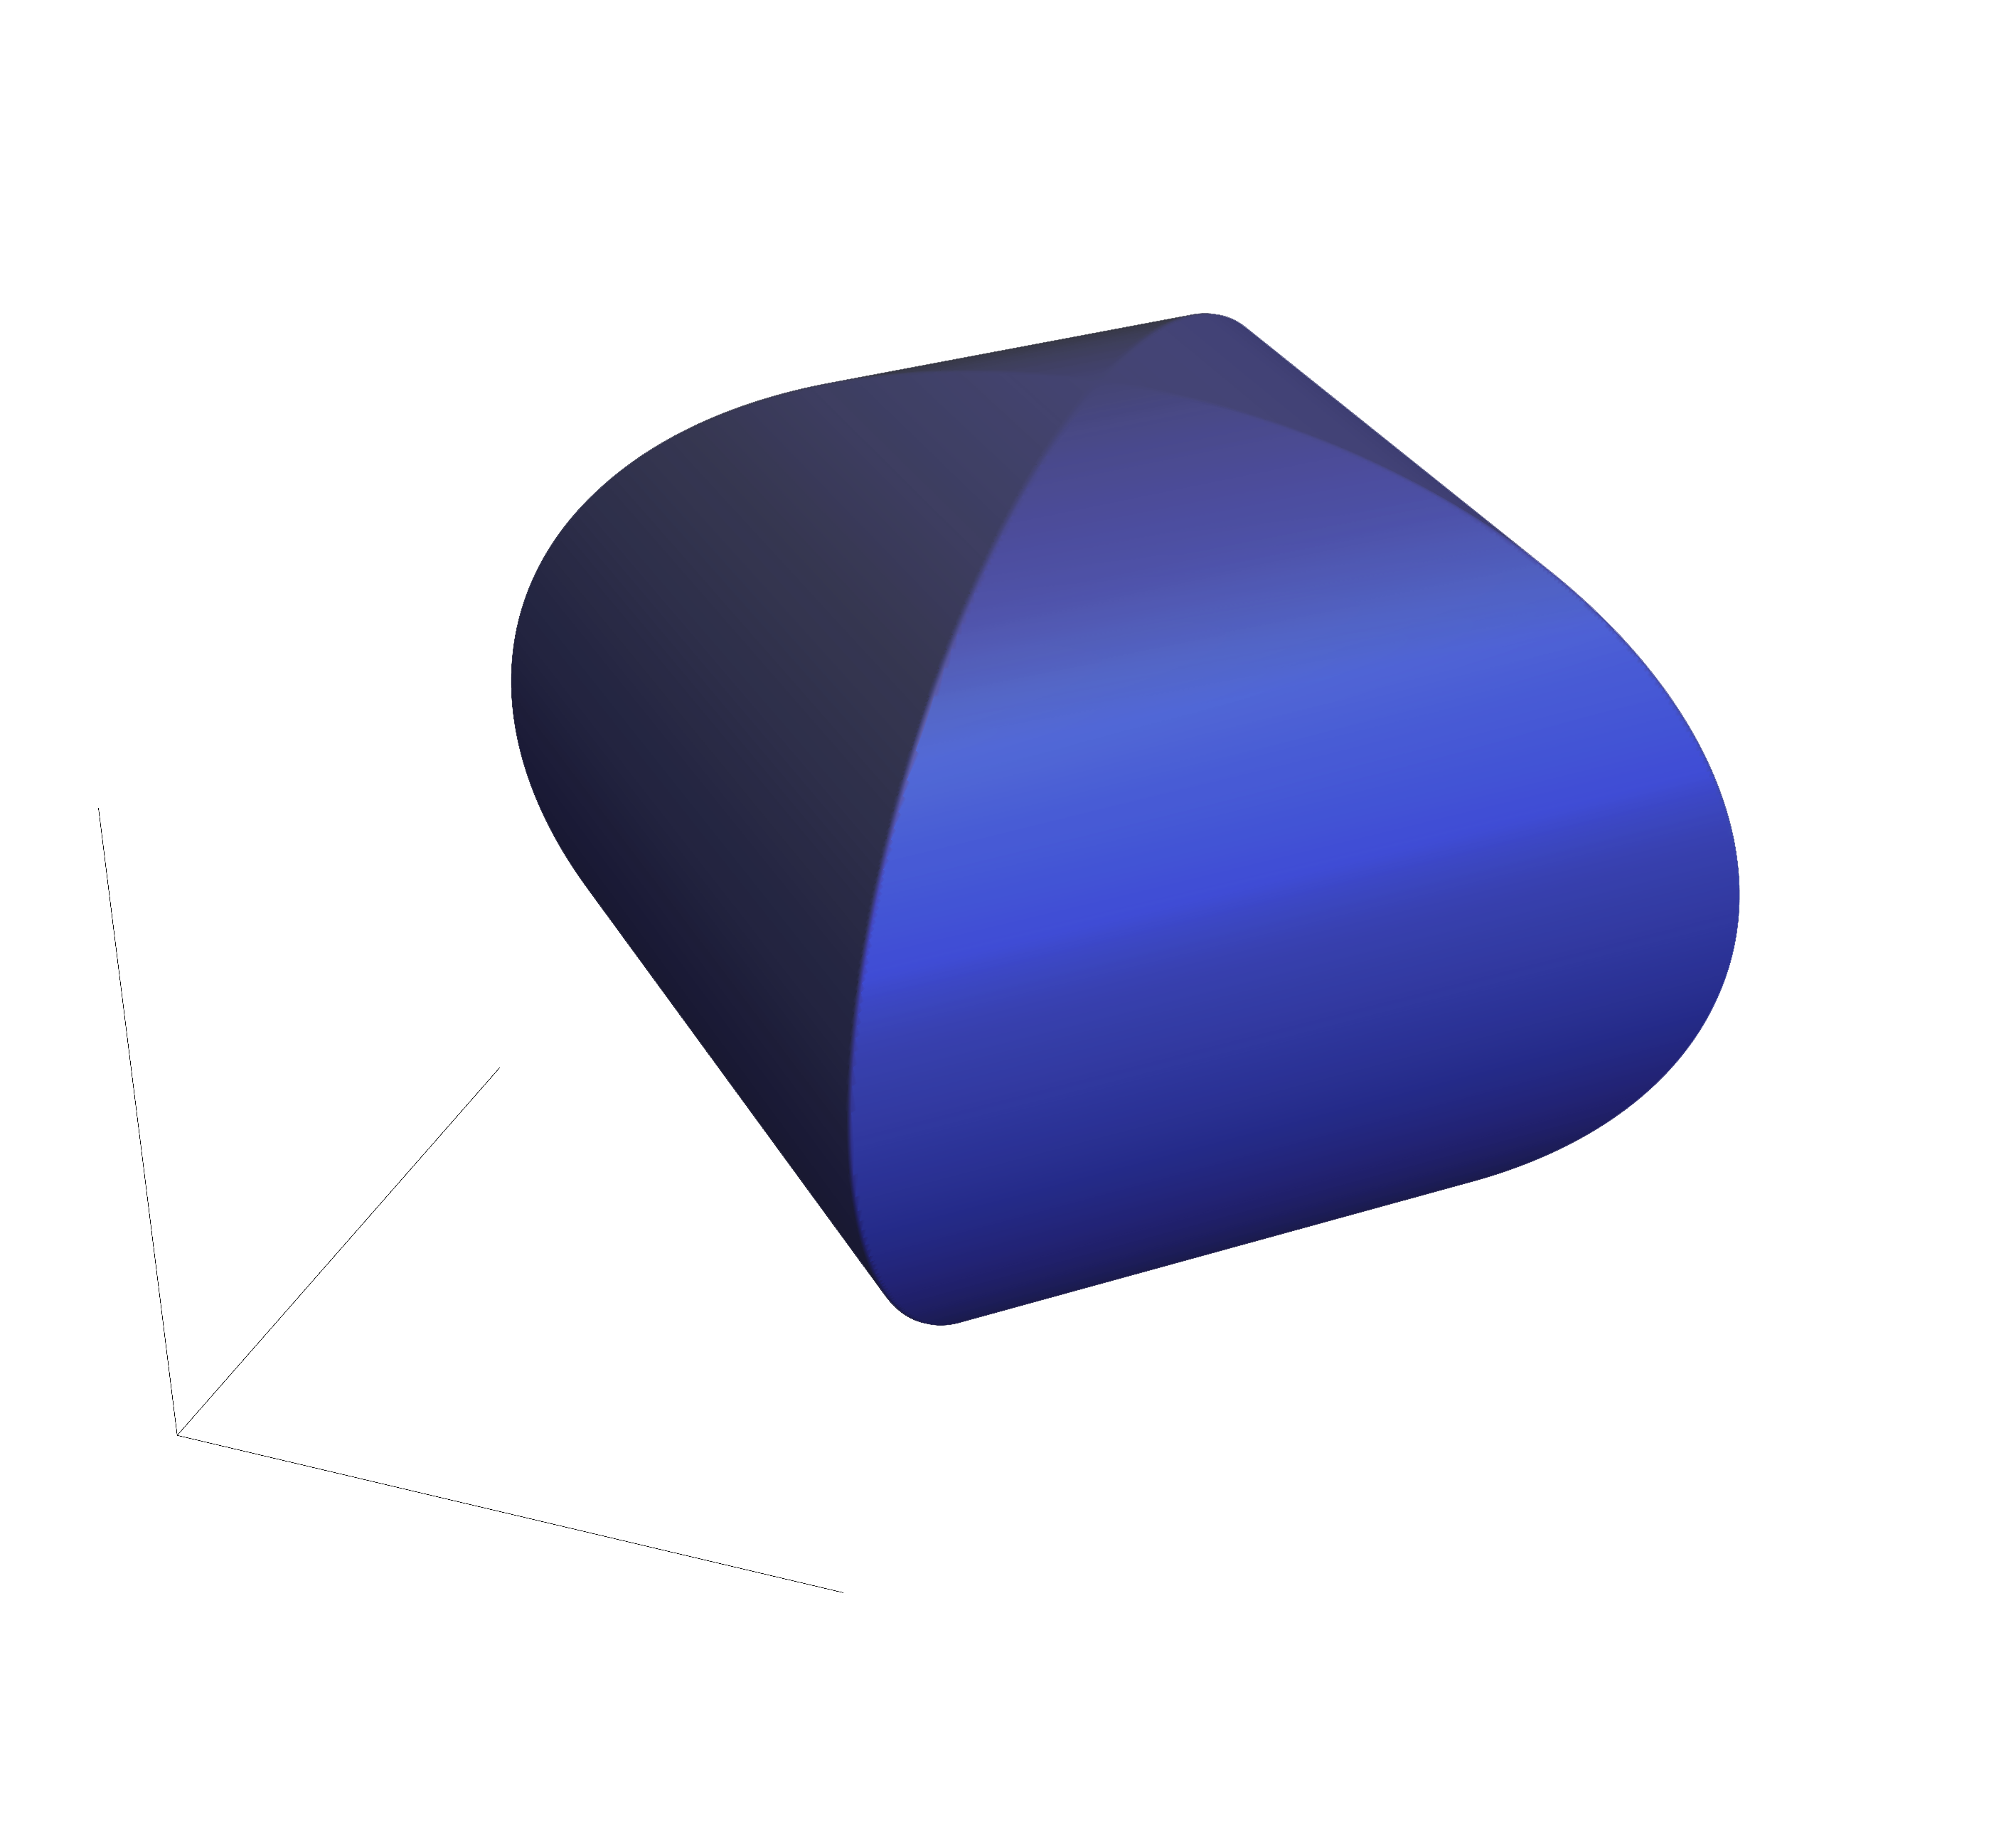
\includegraphics[height=5cm,trim=100 300 380 420,clip]{Evap/BoxTrapEvaporation/SteinmetzEdit}};
    \begin{scope}[x={(image.south east)},y={(image.north west)}]
        \coordinate (Start) at (0.0825,0.165){};
        \draw[-latex] (Start) -- (0.466,0.0515) node [below] {$x$};
        \draw[-latex] (Start) -- (0.27,0.43) node [above] {$y$};
        \draw[-latex] (Start) -- (0.0373,0.615) node [left] {$z$};
    \end{scope}
\end{tikzpicture}
        \caption{$\alpha = \SI{90}{\degree}$}
    \end{subfigure}
    \begin{subfigure}[b]{.49\textwidth}
        \centering
        \usetikzlibrary{arrows,positioning}
\begin{tikzpicture}
    \node[anchor=south west] (image) at (0,0) {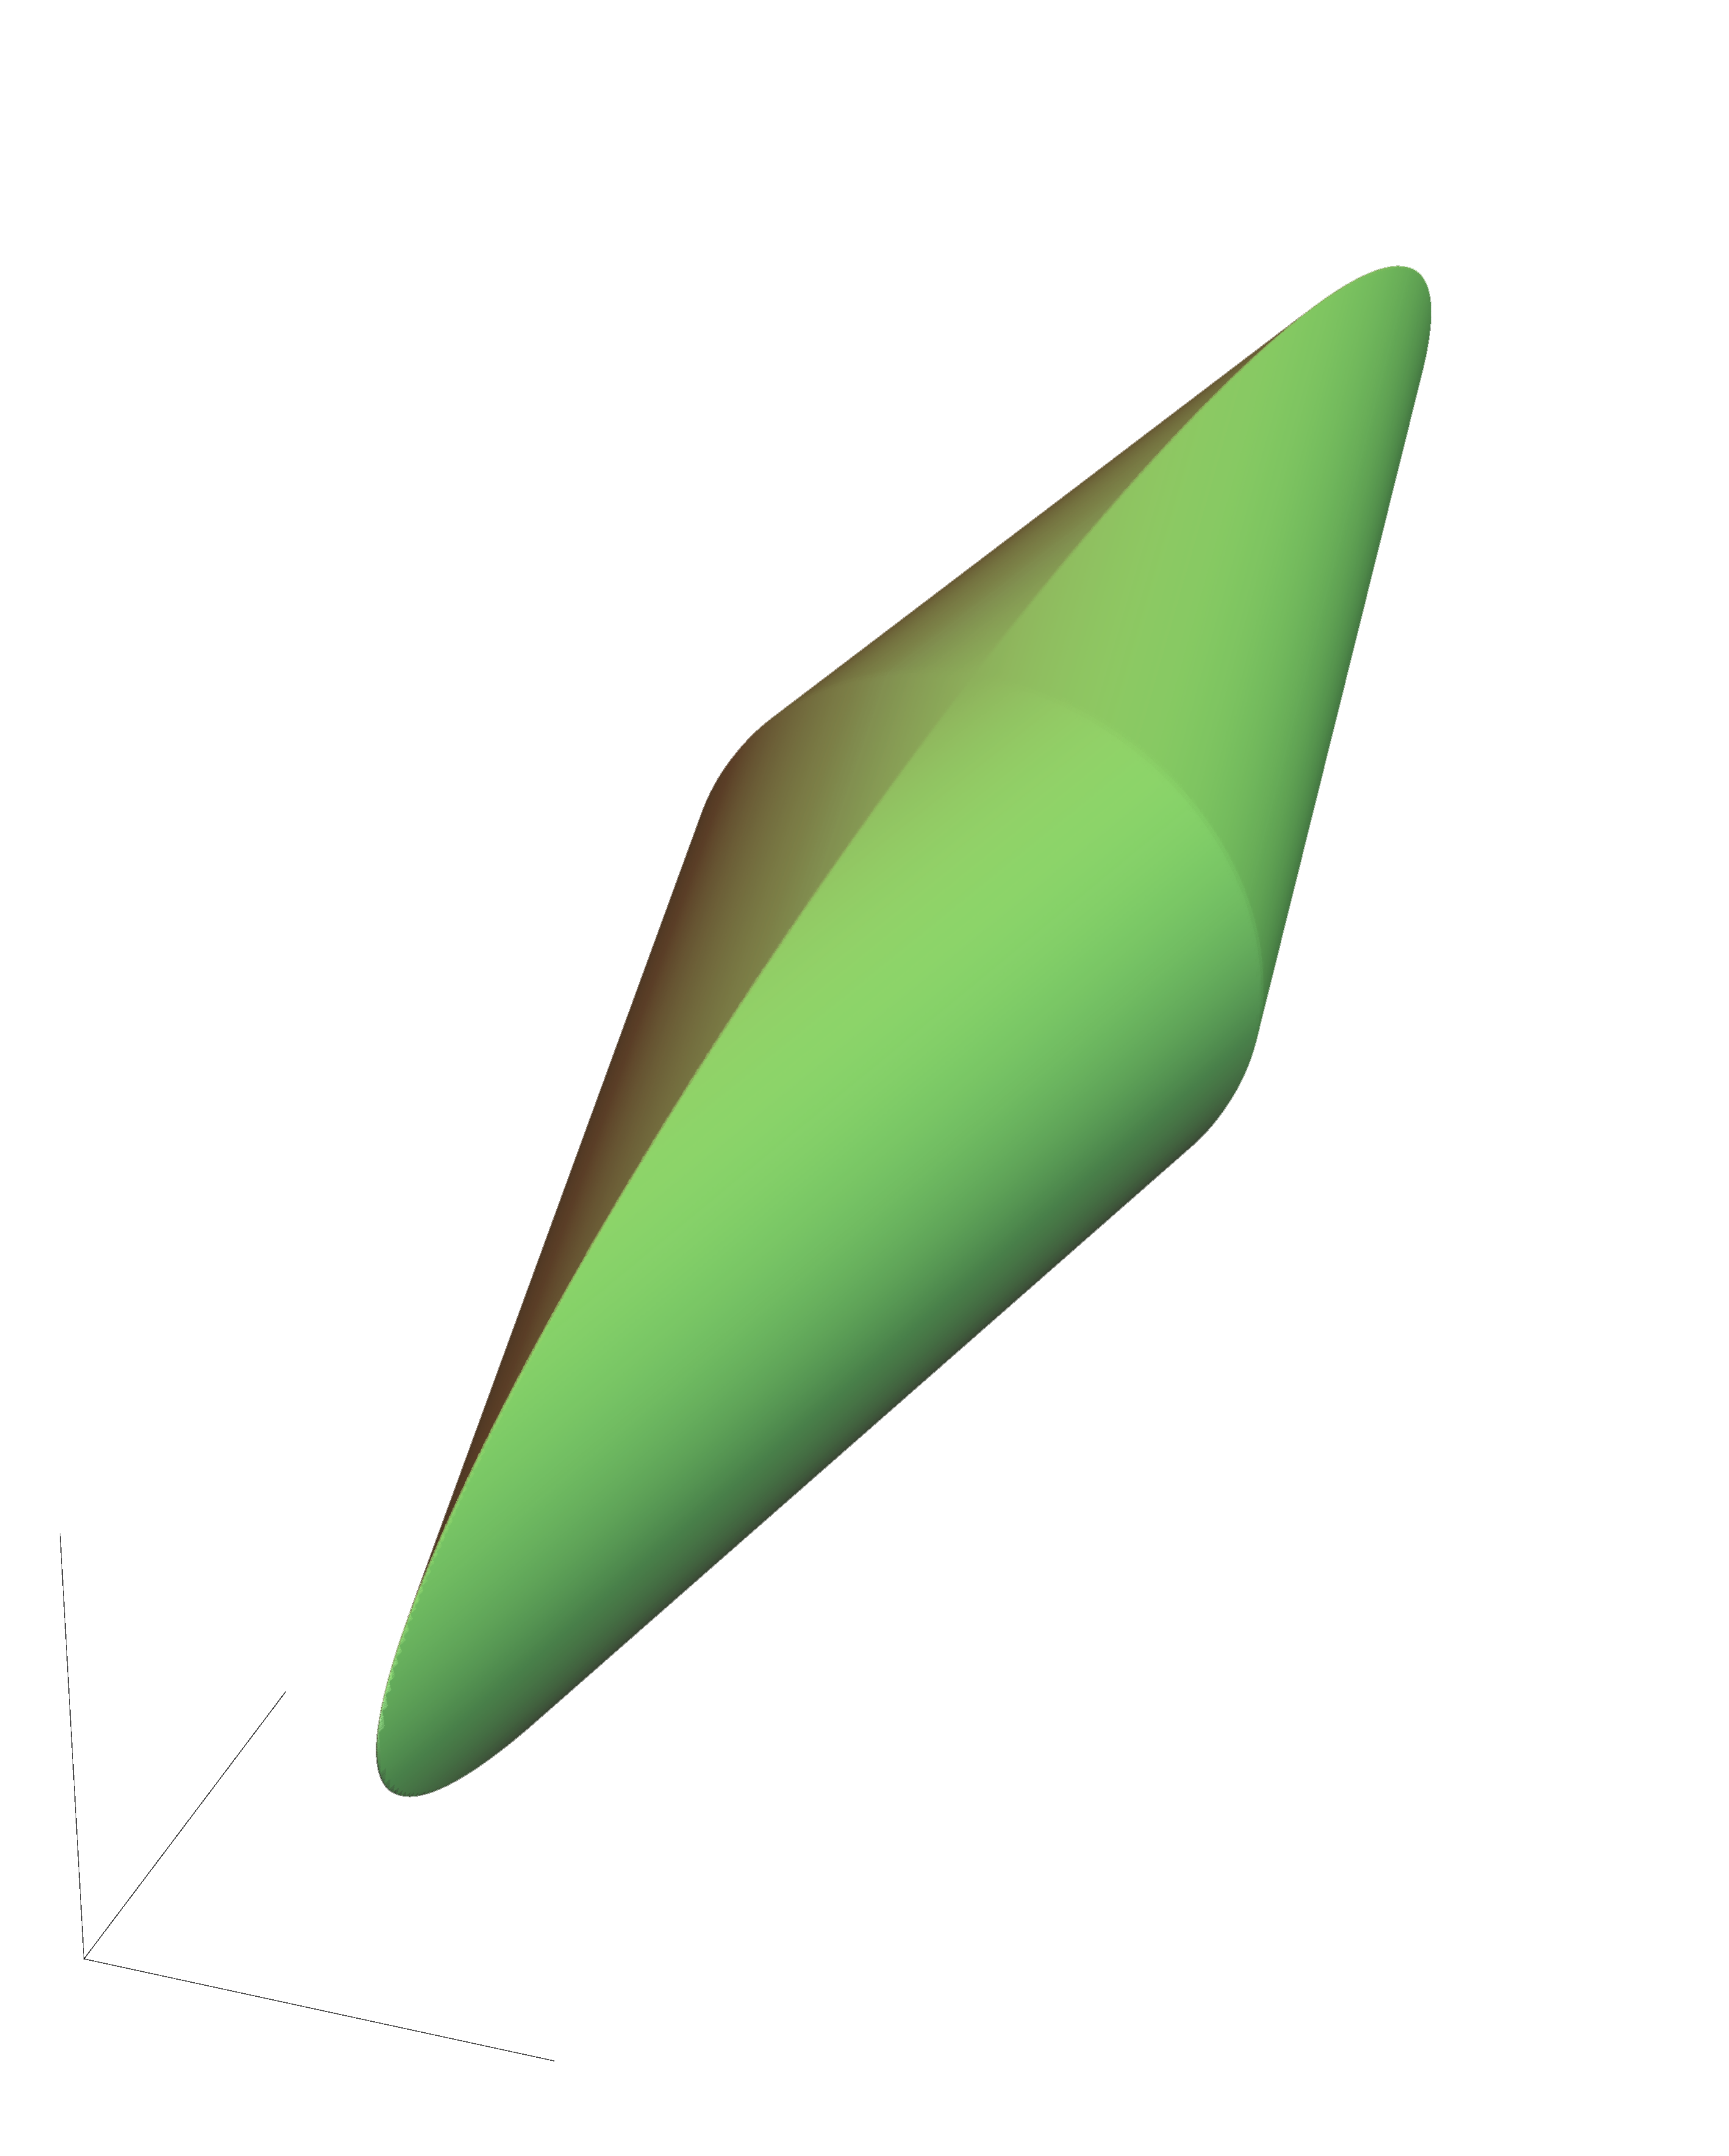
\includegraphics[height=5cm,trim=50 100 470 420,clip]{Evap/BoxTrapEvaporation/SteinmetzAngleEdit}};
    \begin{scope}[x={(image.south east)},y={(image.north west)}]
        \coordinate (Start) at (0.07,0.097){};
        \draw[-latex] (Start) -- (0.383,0.0445) node [below] {$x$};
        \draw[-latex] (Start) -- (0.207,0.238) node [above] {$y$};
        \draw[-latex] (Start) -- (0.0543,0.3175) node [left] {$z$};
    \end{scope}
\end{tikzpicture}
        \caption{$\alpha = \SI{157.5}{\degree}$}
    \end{subfigure}
    \caption[Common volume of two crossed cylinders]{It is important to note that the shapes shown here do not represent an equipotential surface of \cref{eq:eva_potential}. Instead, they simply show the intersection of two cylinders at the two different angles.}
    \label{fig:steinmetz_solid}
\end{figure}
\vfill

% \begin{figure}[htbp]
%     \centering
%     \begin{subfigure}[b]{.49\textwidth}
%         \centering
%         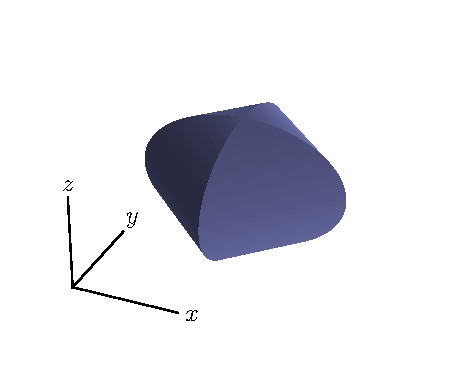
\includegraphics[trim=0 1.7ex 0 6ex,clip]{Evap/SteinMetzPython}
%         \caption{\SI{90}{\degree}}
%     \end{subfigure}
%     \begin{subfigure}[b]{.49\textwidth}
%         \centering
%         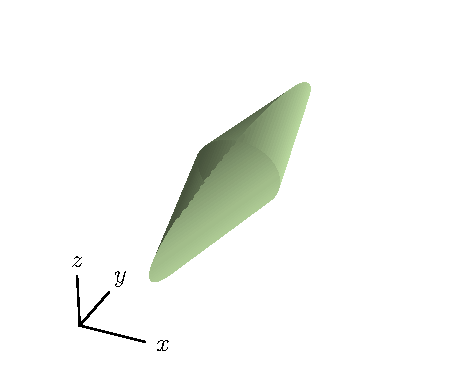
\includegraphics[trim=0 1.7ex 0 6ex,clip]{Evap/SteinMetzPython_Angle}
%         \caption{\SI{157.5}{\degree}}
%     \end{subfigure}
%     \caption{Common volume of two crossed cylinders}
%     \label{fig:steinmetz_solid}
% \end{figure}

\subsubsection*{Parameter Optimisation}
For all cases, we use a simple optimisation scheme. 
The initial beam radius is fixed to \SI{360}{\micro\meter} and the initial trap depth is given by $\SI{50}{\micro\kelvin}\times \kB$. We then employ only one exponential ramp for the beam radius and the potential depth where we compress the beam to a final radius of \SI{25}{\micro\meter} and a final trap depth of $\SI{450}{\nano\kelvin}\times \kB$:
\begin{equation*}
    X(t) = \frac{X_\text{f} - X_\text{i}}{\euler^{-t_\text{d}/\tau} - 1} \times \left(\euler^{-t/\tau} - 1\right) + X_\text{i}.
\end{equation*}
Here, $X$ is the parameter to which the ramp is applied, $X_\text{i,f}$ are the initial and final values before and after the ramp, $t_\text{d}$ is the duration of the ramp and $\tau$ is the exponential time constant.
After an initial coarse search of the available parameter space for $t_\text{d}$ and $\tau$ for both parameters, we choose the values that yield the highest possible evaporation efficiency
\[
    \gamma = -\frac{\log(\tilde{\rho}_\text{f}/\tilde{\rho}_\text{i})}{\log(N_\text{f}/N_\text{i})},
\]
with the initial and final values for the phase space density $\tilde{\rho}_\text{i/f}$ and atom number $N_\text{i/f}$. Then we go on to vary all three parameters ($t_\text{d}$, $\tau$ for the radius $R$ and the trap depth $U_0$) in a smaller range around the previous optimum and try to find an improvement. 

If a phase space density of $\PSD = 1$ is reached, the simulation is stopped prematurely because it is purely classical and results at higher phase space densities are not valid anymore. 

\subsubsection*{Starting Conditions}
We simulate different initial phase space densities ranging from \num{5e-6} to \num{e-3} with atom numbers from \num{2e8} to \num{3e7} as well as temperatures from \SI{10}{\micro\kelvin} down to \SI{2.5}{\micro\kelvin} for the highest phase space density. We initialise the particles with a harmonic density distribution, where the RMS radius can be calculated from the peak phase space density, the atom number and the temperature.
This gives us a range of estimates on how effective this cooling method could be for different starting conditions and we will be able to tell how much pre-cooling is necessary for good results.
The cases with their respective fixed parameters are shown in \cref{tab:evap_cases}.
\begin{table}[bp]
    \centering
    \caption[Initial parameters for the simulated cases]{$\hat{\PSD}$ and $\hat{n}$ are the initial peak phase space and spatial densities, respectively. $\sigma$ is the RMS radius of the initially harmonic cloud.}
    \begin{tabular}{cS[table-format=1.1e-1]S[table-format=1.2]S[table-format=2.1]S[table-format=3]S[table-format=1.1e+2]}
        \toprule
        \# & \multicolumn{1}{c}{$\hat{\PSD}$} & \multicolumn{1}{c}{$N/\num{e8}$} & \multicolumn{1}{c}{$T$/\si{\micro\kelvin}} & \multicolumn{1}{c}{$\sigma$/\si{\micro\meter}} & \multicolumn{1}{c}{$\hat{n}$/\si[per-mode=reciprocal]{\per\meter\cubed}}\\
        \midrule
        1  & 5.0e-6 & 2.00 & 10.0  & 809 & 2.4e16 \\
        2  & 1.9e-5 & 1.20 & 7.1 & 528 & 5.4e16 \\
        3  & 7.1e-5 & 0.77 & 5.0   & 345 & 1.2e17 \\
        4  & 2.7e-4 & 0.48 & 3.5 & 225 & 2.7e17 \\
        5  & 1.0e-3 & 0.30 & 2.5 & 147 & 6.0e17 \\
        \bottomrule
    \end{tabular}
    \label{tab:evap_cases}
\end{table}
% We simulate two different scenarios for both angles: In the first scenario, we assume that the cycling scheme of compression and cooling works. In that case, we start at a phase space density of \todo{number} and a temperature of \todo{number}, corresponding to a density of \todo{number}. Our initial beam radius is given by \todo{number}, so we start with \todo{number} atoms.

% In the second scenario, we do not assume such a great amount of pre-cooling, so we instead start with a phase space density of only \todo{number} at a temperature of \todo{number}, corresponding to the results of \cite{Rosi2018enhancedGM}. At the same initial beam radius, this gives us an initial atom number of \todo{number}.
In all cases, we assume a trap lifetime of \SI{1}{min} (giving $K_1 = \SI{.017}{\per\second}$), no two-body losses and no influence of gravity. This can be achieved in an experiment with a sample prepared in the absolute ground state of $^{87}$Rb where gravity is compensated by a linear magnetic field. The three-body loss coefficient is taken from \cite{threebody} as $K_3 = \SI{1.8e-41}{m^6\per\second}$. At densities below \SI{e19}{\per\meter\cubed}, three body losses are negligible compared to the losses due to background collisions.

\subsubsection*{Findings}
In case 1, the initial density is so low that only a small fraction of the initial atom number can actually be captured in the box. Furthermore, this lower density results in a smaller collision rate and the compression is not fully able to compensate for this. We can achieve efficiencies $\gamma > 2$ only by making the evaporation ramp \SI{30}{s} long. Still, the final phase space density is $\PSD_\text{f}\ll 1$ and less than \num{200000} atoms remain in the trap after the ramp. We can conclude from this that either larger initial trapping beams or a higher initial density would be necessary.

At initial phase space densities above $\num{e-5}$, the situation improves drastically and efficiencies close to or above 3 can be achieved. However, this comes again at the expense of long ramp durations.

The results for all five cases are listed in \cref{tab:evap_results} and \cref{fig:evap_comparison} shows a comparison of the cases 2--5 against various results from other research groups. Here we can see that our achieved efficiency can compete with the compared results. In the cases 4 and 5, a large portion of the atoms remains in the trap at a phase space density of $\PSD = 1$. We also find that the achieved efficiency is very dependent on the initial atom number. This is expected as the initial atom number determines how strong the compression needs to be to achieve high densities and in turn high collision rates.

Lastly, we show the optimised trajectory for case 5 in \cref{fig:evap_trajectory}. During the first second of compression, no evaporation takes place, which is apparent by the relatively constant atom number and phase space density. Starting at a lower trap depth might reduce the total time necessary to reach $\PSD = 1$.

The trajectories for the other cases can be found in \cref{fig:eva_cases14}.
%
% \begin{table}[bp]
%     \centering
%     \caption{Results and optimised parameters for the simulated cases}
%     \begin{tabular}{cS[table-format=1.1e+1]S[table-format=1.1e+1]S[table-format=1.1e-1]S[table-format=1.3]S[table-format=2.1]S[table-format=3]S[table-format=1.2]}
%         \toprule
%         \# & \multicolumn{1}{c}{$N_\text{i}$} & \multicolumn{1}{c}{$N_\text{f}$} & \multicolumn{1}{c}{$\PSD_\text{i}$} & \multicolumn{1}{c}{$\PSD_\text{f}$} & \multicolumn{1}{c}{$T_\text{i}$/\si{\micro\kelvin}} & \multicolumn{1}{c}{$T_\text{f}$/\si{\nano\kelvin}} & \multicolumn{1}{c}{$\gamma$} \\
%         \midrule
%         1  & 1.1e7 & 1.3e5 & 3.7e-6 & 0.059  & 10 & 152 & 2.17 \\
%         2  & 1.9e7 & 5.5e5 & 1.2e-5 & 0.29 & 7.0 & 137 & 2.83 \\
%         3  & 2.8e7 & 1.3e6 & 3.9e-5 & 0.83 & 5.0 & 185 & 3.20 \\
%         4  & 3.3e7 & 2.0e6 & 1.2e-4 & 1    & 3.6 & 144 & 3.25 \\
%         5  & 2.8e7 & 2.3e6 & 3.4e-4 & 1    & 2.5 & 160 & 3.21 \\
%         \bottomrule
%     \end{tabular}
%     \newline
%     \vspace{3ex}
%     \newline
%     \begin{tabular}{cS[table-format=2.0]S[table-format=1.1]S[table-format=2.1]}
%         \toprule
%         \# & \multicolumn{1}{c}{$t_\text{d}$/s} & \multicolumn{1}{c}{$\tau_R$/s} & \multicolumn{1}{c}{$\tau_{U_0}$/s} \\
%         \midrule
%         1  & 30 & 4 & 30 \\
%         2  & 16 & 1.6 & 15 \\
%         3  & 14 & 1.4 & 13 \\
%         4  & 9 & 0.9 & 8.5 \\
%         5  & 7 & 0.7 & 6.5 \\
%         \bottomrule
%     \end{tabular}
%     \label{tab:evap_results}
% \end{table}
%

\clearpage
\vbox{
\noindent\begin{minipage}[c][.7518\textheight][t]{\textwidth}   

% \begin{figure}[tp]
    % \centering
    % \begin{minipage}{1\textwidth}
        %% Creator: Matplotlib, PGF backend
%%
%% To include the figure in your LaTeX document, write
%%   \input{<filename>.pgf}
%%
%% Make sure the required packages are loaded in your preamble
%%   \usepackage{pgf}
%%
%% and, on pdftex
%%   \usepackage[utf8]{inputenc}\DeclareUnicodeCharacter{2212}{-}
%%
%% or, on luatex and xetex
%%   \usepackage{unicode-math}
%%
%% Figures using additional raster images can only be included by \input if
%% they are in the same directory as the main LaTeX file. For loading figures
%% from other directories you can use the `import` package
%%   \usepackage{import}
%%
%% and then include the figures with
%%   \import{<path to file>}{<filename>.pgf}
%%
%% Matplotlib used the following preamble
%%   \usepackage[utf8]{inputenc}
%%   \usepackage[T1]{fontenc}
%%   \usepackage[detect-all,locale=UK]{siunitx}
%%   \usepackage{amsmath}
%%   \usepackage{lmodern}
%%   \DeclareUnicodeCharacter{2212}{$-$}
%%
\begingroup%
\makeatletter%
\begin{pgfpicture}%
\pgfpathrectangle{\pgfpointorigin}{\pgfqpoint{6.134381in}{5.042466in}}%
\pgfusepath{use as bounding box, clip}%
\begin{pgfscope}%
\pgfsetbuttcap%
\pgfsetmiterjoin%
\definecolor{currentfill}{rgb}{1.000000,1.000000,1.000000}%
\pgfsetfillcolor{currentfill}%
\pgfsetlinewidth{0.000000pt}%
\definecolor{currentstroke}{rgb}{1.000000,1.000000,1.000000}%
\pgfsetstrokecolor{currentstroke}%
\pgfsetdash{}{0pt}%
\pgfpathmoveto{\pgfqpoint{0.000000in}{0.000000in}}%
\pgfpathlineto{\pgfqpoint{6.134381in}{0.000000in}}%
\pgfpathlineto{\pgfqpoint{6.134381in}{5.042466in}}%
\pgfpathlineto{\pgfqpoint{0.000000in}{5.042466in}}%
\pgfpathclose%
\pgfusepath{fill}%
\end{pgfscope}%
\begin{pgfscope}%
\pgfsetbuttcap%
\pgfsetmiterjoin%
\definecolor{currentfill}{rgb}{1.000000,1.000000,1.000000}%
\pgfsetfillcolor{currentfill}%
\pgfsetlinewidth{0.000000pt}%
\definecolor{currentstroke}{rgb}{0.000000,0.000000,0.000000}%
\pgfsetstrokecolor{currentstroke}%
\pgfsetstrokeopacity{0.000000}%
\pgfsetdash{}{0pt}%
\pgfpathmoveto{\pgfqpoint{0.566079in}{2.406301in}}%
\pgfpathlineto{\pgfqpoint{3.023396in}{2.406301in}}%
\pgfpathlineto{\pgfqpoint{3.023396in}{4.284350in}}%
\pgfpathlineto{\pgfqpoint{0.566079in}{4.284350in}}%
\pgfpathclose%
\pgfusepath{fill}%
\end{pgfscope}%
\begin{pgfscope}%
\pgfpathrectangle{\pgfqpoint{0.566079in}{2.406301in}}{\pgfqpoint{2.457317in}{1.878049in}}%
\pgfusepath{clip}%
\pgfsetbuttcap%
\pgfsetroundjoin%
\definecolor{currentfill}{rgb}{0.312566,0.691372,0.493273}%
\pgfsetfillcolor{currentfill}%
\pgfsetlinewidth{1.003750pt}%
\definecolor{currentstroke}{rgb}{0.312566,0.691372,0.493273}%
\pgfsetstrokecolor{currentstroke}%
\pgfsetdash{}{0pt}%
\pgfsys@defobject{currentmarker}{\pgfqpoint{-0.038036in}{-0.038036in}}{\pgfqpoint{0.038036in}{0.038036in}}{%
\pgfpathmoveto{\pgfqpoint{0.000000in}{-0.038036in}}%
\pgfpathcurveto{\pgfqpoint{0.010087in}{-0.038036in}}{\pgfqpoint{0.019763in}{-0.034029in}}{\pgfqpoint{0.026896in}{-0.026896in}}%
\pgfpathcurveto{\pgfqpoint{0.034029in}{-0.019763in}}{\pgfqpoint{0.038036in}{-0.010087in}}{\pgfqpoint{0.038036in}{0.000000in}}%
\pgfpathcurveto{\pgfqpoint{0.038036in}{0.010087in}}{\pgfqpoint{0.034029in}{0.019763in}}{\pgfqpoint{0.026896in}{0.026896in}}%
\pgfpathcurveto{\pgfqpoint{0.019763in}{0.034029in}}{\pgfqpoint{0.010087in}{0.038036in}}{\pgfqpoint{0.000000in}{0.038036in}}%
\pgfpathcurveto{\pgfqpoint{-0.010087in}{0.038036in}}{\pgfqpoint{-0.019763in}{0.034029in}}{\pgfqpoint{-0.026896in}{0.026896in}}%
\pgfpathcurveto{\pgfqpoint{-0.034029in}{0.019763in}}{\pgfqpoint{-0.038036in}{0.010087in}}{\pgfqpoint{-0.038036in}{0.000000in}}%
\pgfpathcurveto{\pgfqpoint{-0.038036in}{-0.010087in}}{\pgfqpoint{-0.034029in}{-0.019763in}}{\pgfqpoint{-0.026896in}{-0.026896in}}%
\pgfpathcurveto{\pgfqpoint{-0.019763in}{-0.034029in}}{\pgfqpoint{-0.010087in}{-0.038036in}}{\pgfqpoint{0.000000in}{-0.038036in}}%
\pgfpathclose%
\pgfusepath{stroke,fill}%
}%
\begin{pgfscope}%
\pgfsys@transformshift{0.677775in}{3.198775in}%
\pgfsys@useobject{currentmarker}{}%
\end{pgfscope}%
\end{pgfscope}%
\begin{pgfscope}%
\pgfpathrectangle{\pgfqpoint{0.566079in}{2.406301in}}{\pgfqpoint{2.457317in}{1.878049in}}%
\pgfusepath{clip}%
\pgfsetbuttcap%
\pgfsetroundjoin%
\definecolor{currentfill}{rgb}{0.312566,0.691372,0.493273}%
\pgfsetfillcolor{currentfill}%
\pgfsetlinewidth{1.003750pt}%
\definecolor{currentstroke}{rgb}{0.312566,0.691372,0.493273}%
\pgfsetstrokecolor{currentstroke}%
\pgfsetdash{}{0pt}%
\pgfsys@defobject{currentmarker}{\pgfqpoint{-0.038036in}{-0.038036in}}{\pgfqpoint{0.038036in}{0.038036in}}{%
\pgfpathmoveto{\pgfqpoint{0.000000in}{-0.038036in}}%
\pgfpathcurveto{\pgfqpoint{0.010087in}{-0.038036in}}{\pgfqpoint{0.019763in}{-0.034029in}}{\pgfqpoint{0.026896in}{-0.026896in}}%
\pgfpathcurveto{\pgfqpoint{0.034029in}{-0.019763in}}{\pgfqpoint{0.038036in}{-0.010087in}}{\pgfqpoint{0.038036in}{0.000000in}}%
\pgfpathcurveto{\pgfqpoint{0.038036in}{0.010087in}}{\pgfqpoint{0.034029in}{0.019763in}}{\pgfqpoint{0.026896in}{0.026896in}}%
\pgfpathcurveto{\pgfqpoint{0.019763in}{0.034029in}}{\pgfqpoint{0.010087in}{0.038036in}}{\pgfqpoint{0.000000in}{0.038036in}}%
\pgfpathcurveto{\pgfqpoint{-0.010087in}{0.038036in}}{\pgfqpoint{-0.019763in}{0.034029in}}{\pgfqpoint{-0.026896in}{0.026896in}}%
\pgfpathcurveto{\pgfqpoint{-0.034029in}{0.019763in}}{\pgfqpoint{-0.038036in}{0.010087in}}{\pgfqpoint{-0.038036in}{0.000000in}}%
\pgfpathcurveto{\pgfqpoint{-0.038036in}{-0.010087in}}{\pgfqpoint{-0.034029in}{-0.019763in}}{\pgfqpoint{-0.026896in}{-0.026896in}}%
\pgfpathcurveto{\pgfqpoint{-0.019763in}{-0.034029in}}{\pgfqpoint{-0.010087in}{-0.038036in}}{\pgfqpoint{0.000000in}{-0.038036in}}%
\pgfpathclose%
\pgfusepath{stroke,fill}%
}%
\begin{pgfscope}%
\pgfsys@transformshift{0.975629in}{3.764498in}%
\pgfsys@useobject{currentmarker}{}%
\end{pgfscope}%
\end{pgfscope}%
\begin{pgfscope}%
\pgfpathrectangle{\pgfqpoint{0.566079in}{2.406301in}}{\pgfqpoint{2.457317in}{1.878049in}}%
\pgfusepath{clip}%
\pgfsetbuttcap%
\pgfsetroundjoin%
\definecolor{currentfill}{rgb}{0.312566,0.691372,0.493273}%
\pgfsetfillcolor{currentfill}%
\pgfsetlinewidth{1.003750pt}%
\definecolor{currentstroke}{rgb}{0.312566,0.691372,0.493273}%
\pgfsetstrokecolor{currentstroke}%
\pgfsetdash{}{0pt}%
\pgfsys@defobject{currentmarker}{\pgfqpoint{-0.038036in}{-0.038036in}}{\pgfqpoint{0.038036in}{0.038036in}}{%
\pgfpathmoveto{\pgfqpoint{0.000000in}{-0.038036in}}%
\pgfpathcurveto{\pgfqpoint{0.010087in}{-0.038036in}}{\pgfqpoint{0.019763in}{-0.034029in}}{\pgfqpoint{0.026896in}{-0.026896in}}%
\pgfpathcurveto{\pgfqpoint{0.034029in}{-0.019763in}}{\pgfqpoint{0.038036in}{-0.010087in}}{\pgfqpoint{0.038036in}{0.000000in}}%
\pgfpathcurveto{\pgfqpoint{0.038036in}{0.010087in}}{\pgfqpoint{0.034029in}{0.019763in}}{\pgfqpoint{0.026896in}{0.026896in}}%
\pgfpathcurveto{\pgfqpoint{0.019763in}{0.034029in}}{\pgfqpoint{0.010087in}{0.038036in}}{\pgfqpoint{0.000000in}{0.038036in}}%
\pgfpathcurveto{\pgfqpoint{-0.010087in}{0.038036in}}{\pgfqpoint{-0.019763in}{0.034029in}}{\pgfqpoint{-0.026896in}{0.026896in}}%
\pgfpathcurveto{\pgfqpoint{-0.034029in}{0.019763in}}{\pgfqpoint{-0.038036in}{0.010087in}}{\pgfqpoint{-0.038036in}{0.000000in}}%
\pgfpathcurveto{\pgfqpoint{-0.038036in}{-0.010087in}}{\pgfqpoint{-0.034029in}{-0.019763in}}{\pgfqpoint{-0.026896in}{-0.026896in}}%
\pgfpathcurveto{\pgfqpoint{-0.019763in}{-0.034029in}}{\pgfqpoint{-0.010087in}{-0.038036in}}{\pgfqpoint{0.000000in}{-0.038036in}}%
\pgfpathclose%
\pgfusepath{stroke,fill}%
}%
\begin{pgfscope}%
\pgfsys@transformshift{0.677775in}{3.454294in}%
\pgfsys@useobject{currentmarker}{}%
\end{pgfscope}%
\end{pgfscope}%
\begin{pgfscope}%
\pgfpathrectangle{\pgfqpoint{0.566079in}{2.406301in}}{\pgfqpoint{2.457317in}{1.878049in}}%
\pgfusepath{clip}%
\pgfsetbuttcap%
\pgfsetroundjoin%
\definecolor{currentfill}{rgb}{0.145643,0.174529,0.638669}%
\pgfsetfillcolor{currentfill}%
\pgfsetlinewidth{1.003750pt}%
\definecolor{currentstroke}{rgb}{0.145643,0.174529,0.638669}%
\pgfsetstrokecolor{currentstroke}%
\pgfsetdash{}{0pt}%
\pgfsys@defobject{currentmarker}{\pgfqpoint{-0.038036in}{-0.038036in}}{\pgfqpoint{0.038036in}{0.038036in}}{%
\pgfpathmoveto{\pgfqpoint{-0.038036in}{-0.038036in}}%
\pgfpathlineto{\pgfqpoint{0.038036in}{-0.038036in}}%
\pgfpathlineto{\pgfqpoint{0.038036in}{0.038036in}}%
\pgfpathlineto{\pgfqpoint{-0.038036in}{0.038036in}}%
\pgfpathclose%
\pgfusepath{stroke,fill}%
}%
\begin{pgfscope}%
\pgfsys@transformshift{0.677775in}{3.865076in}%
\pgfsys@useobject{currentmarker}{}%
\end{pgfscope}%
\end{pgfscope}%
\begin{pgfscope}%
\pgfpathrectangle{\pgfqpoint{0.566079in}{2.406301in}}{\pgfqpoint{2.457317in}{1.878049in}}%
\pgfusepath{clip}%
\pgfsetbuttcap%
\pgfsetroundjoin%
\definecolor{currentfill}{rgb}{0.082916,0.386480,0.554994}%
\pgfsetfillcolor{currentfill}%
\pgfsetlinewidth{1.003750pt}%
\definecolor{currentstroke}{rgb}{0.082916,0.386480,0.554994}%
\pgfsetstrokecolor{currentstroke}%
\pgfsetdash{}{0pt}%
\pgfsys@defobject{currentmarker}{\pgfqpoint{-0.053791in}{-0.053791in}}{\pgfqpoint{0.053791in}{0.053791in}}{%
\pgfpathmoveto{\pgfqpoint{-0.000000in}{-0.053791in}}%
\pgfpathlineto{\pgfqpoint{0.053791in}{0.000000in}}%
\pgfpathlineto{\pgfqpoint{0.000000in}{0.053791in}}%
\pgfpathlineto{\pgfqpoint{-0.053791in}{0.000000in}}%
\pgfpathclose%
\pgfusepath{stroke,fill}%
}%
\begin{pgfscope}%
\pgfsys@transformshift{2.018118in}{2.491667in}%
\pgfsys@useobject{currentmarker}{}%
\end{pgfscope}%
\end{pgfscope}%
\begin{pgfscope}%
\pgfpathrectangle{\pgfqpoint{0.566079in}{2.406301in}}{\pgfqpoint{2.457317in}{1.878049in}}%
\pgfusepath{clip}%
\pgfsetbuttcap%
\pgfsetroundjoin%
\pgfsetlinewidth{2.007500pt}%
\definecolor{currentstroke}{rgb}{0.581062,0.828765,0.366380}%
\pgfsetstrokecolor{currentstroke}%
\pgfsetdash{}{0pt}%
\pgfpathmoveto{\pgfqpoint{2.911700in}{3.377724in}}%
\pgfpathcurveto{\pgfqpoint{2.921787in}{3.377724in}}{\pgfqpoint{2.931463in}{3.381732in}}{\pgfqpoint{2.938595in}{3.388864in}}%
\pgfpathcurveto{\pgfqpoint{2.945728in}{3.395997in}}{\pgfqpoint{2.949736in}{3.405673in}}{\pgfqpoint{2.949736in}{3.415760in}}%
\pgfpathcurveto{\pgfqpoint{2.949736in}{3.425848in}}{\pgfqpoint{2.945728in}{3.435523in}}{\pgfqpoint{2.938595in}{3.442656in}}%
\pgfpathcurveto{\pgfqpoint{2.931463in}{3.449789in}}{\pgfqpoint{2.921787in}{3.453796in}}{\pgfqpoint{2.911700in}{3.453796in}}%
\pgfpathcurveto{\pgfqpoint{2.901612in}{3.453796in}}{\pgfqpoint{2.891937in}{3.449789in}}{\pgfqpoint{2.884804in}{3.442656in}}%
\pgfpathcurveto{\pgfqpoint{2.877671in}{3.435523in}}{\pgfqpoint{2.873663in}{3.425848in}}{\pgfqpoint{2.873663in}{3.415760in}}%
\pgfpathcurveto{\pgfqpoint{2.873663in}{3.405673in}}{\pgfqpoint{2.877671in}{3.395997in}}{\pgfqpoint{2.884804in}{3.388864in}}%
\pgfpathcurveto{\pgfqpoint{2.891937in}{3.381732in}}{\pgfqpoint{2.901612in}{3.377724in}}{\pgfqpoint{2.911700in}{3.377724in}}%
\pgfpathclose%
\pgfusepath{stroke}%
\end{pgfscope}%
\begin{pgfscope}%
\pgfpathrectangle{\pgfqpoint{0.566079in}{2.406301in}}{\pgfqpoint{2.457317in}{1.878049in}}%
\pgfusepath{clip}%
\pgfsetbuttcap%
\pgfsetroundjoin%
\pgfsetlinewidth{2.007500pt}%
\definecolor{currentstroke}{rgb}{0.581062,0.828765,0.366380}%
\pgfsetstrokecolor{currentstroke}%
\pgfsetdash{}{0pt}%
\pgfpathmoveto{\pgfqpoint{2.613842in}{4.060042in}}%
\pgfpathcurveto{\pgfqpoint{2.623929in}{4.060042in}}{\pgfqpoint{2.633605in}{4.064050in}}{\pgfqpoint{2.640737in}{4.071183in}}%
\pgfpathcurveto{\pgfqpoint{2.647870in}{4.078316in}}{\pgfqpoint{2.651878in}{4.087991in}}{\pgfqpoint{2.651878in}{4.098079in}}%
\pgfpathcurveto{\pgfqpoint{2.651878in}{4.108166in}}{\pgfqpoint{2.647870in}{4.117842in}}{\pgfqpoint{2.640737in}{4.124974in}}%
\pgfpathcurveto{\pgfqpoint{2.633605in}{4.132107in}}{\pgfqpoint{2.623929in}{4.136115in}}{\pgfqpoint{2.613842in}{4.136115in}}%
\pgfpathcurveto{\pgfqpoint{2.603754in}{4.136115in}}{\pgfqpoint{2.594079in}{4.132107in}}{\pgfqpoint{2.586946in}{4.124974in}}%
\pgfpathcurveto{\pgfqpoint{2.579813in}{4.117842in}}{\pgfqpoint{2.575805in}{4.108166in}}{\pgfqpoint{2.575805in}{4.098079in}}%
\pgfpathcurveto{\pgfqpoint{2.575805in}{4.087991in}}{\pgfqpoint{2.579813in}{4.078316in}}{\pgfqpoint{2.586946in}{4.071183in}}%
\pgfpathcurveto{\pgfqpoint{2.594079in}{4.064050in}}{\pgfqpoint{2.603754in}{4.060042in}}{\pgfqpoint{2.613842in}{4.060042in}}%
\pgfpathclose%
\pgfusepath{stroke}%
\end{pgfscope}%
\begin{pgfscope}%
\pgfpathrectangle{\pgfqpoint{0.566079in}{2.406301in}}{\pgfqpoint{2.457317in}{1.878049in}}%
\pgfusepath{clip}%
\pgfsetbuttcap%
\pgfsetroundjoin%
\pgfsetlinewidth{2.007500pt}%
\definecolor{currentstroke}{rgb}{0.581062,0.828765,0.366380}%
\pgfsetstrokecolor{currentstroke}%
\pgfsetdash{}{0pt}%
\pgfpathmoveto{\pgfqpoint{1.865049in}{4.160948in}}%
\pgfpathcurveto{\pgfqpoint{1.875137in}{4.160948in}}{\pgfqpoint{1.884812in}{4.164955in}}{\pgfqpoint{1.891945in}{4.172088in}}%
\pgfpathcurveto{\pgfqpoint{1.899078in}{4.179221in}}{\pgfqpoint{1.903086in}{4.188897in}}{\pgfqpoint{1.903086in}{4.198984in}}%
\pgfpathcurveto{\pgfqpoint{1.903086in}{4.209071in}}{\pgfqpoint{1.899078in}{4.218747in}}{\pgfqpoint{1.891945in}{4.225880in}}%
\pgfpathcurveto{\pgfqpoint{1.884812in}{4.233012in}}{\pgfqpoint{1.875137in}{4.237020in}}{\pgfqpoint{1.865049in}{4.237020in}}%
\pgfpathcurveto{\pgfqpoint{1.854962in}{4.237020in}}{\pgfqpoint{1.845286in}{4.233012in}}{\pgfqpoint{1.838154in}{4.225880in}}%
\pgfpathcurveto{\pgfqpoint{1.831021in}{4.218747in}}{\pgfqpoint{1.827013in}{4.209071in}}{\pgfqpoint{1.827013in}{4.198984in}}%
\pgfpathcurveto{\pgfqpoint{1.827013in}{4.188897in}}{\pgfqpoint{1.831021in}{4.179221in}}{\pgfqpoint{1.838154in}{4.172088in}}%
\pgfpathcurveto{\pgfqpoint{1.845286in}{4.164955in}}{\pgfqpoint{1.854962in}{4.160948in}}{\pgfqpoint{1.865049in}{4.160948in}}%
\pgfpathclose%
\pgfusepath{stroke}%
\end{pgfscope}%
\begin{pgfscope}%
\pgfpathrectangle{\pgfqpoint{0.566079in}{2.406301in}}{\pgfqpoint{2.457317in}{1.878049in}}%
\pgfusepath{clip}%
\pgfsetbuttcap%
\pgfsetroundjoin%
\pgfsetlinewidth{2.007500pt}%
\definecolor{currentstroke}{rgb}{0.581062,0.828765,0.366380}%
\pgfsetstrokecolor{currentstroke}%
\pgfsetdash{}{0pt}%
\pgfpathmoveto{\pgfqpoint{1.565366in}{4.081237in}}%
\pgfpathcurveto{\pgfqpoint{1.575453in}{4.081237in}}{\pgfqpoint{1.585129in}{4.085245in}}{\pgfqpoint{1.592262in}{4.092377in}}%
\pgfpathcurveto{\pgfqpoint{1.599394in}{4.099510in}}{\pgfqpoint{1.603402in}{4.109186in}}{\pgfqpoint{1.603402in}{4.119273in}}%
\pgfpathcurveto{\pgfqpoint{1.603402in}{4.129360in}}{\pgfqpoint{1.599394in}{4.139036in}}{\pgfqpoint{1.592262in}{4.146169in}}%
\pgfpathcurveto{\pgfqpoint{1.585129in}{4.153302in}}{\pgfqpoint{1.575453in}{4.157309in}}{\pgfqpoint{1.565366in}{4.157309in}}%
\pgfpathcurveto{\pgfqpoint{1.555278in}{4.157309in}}{\pgfqpoint{1.545603in}{4.153302in}}{\pgfqpoint{1.538470in}{4.146169in}}%
\pgfpathcurveto{\pgfqpoint{1.531337in}{4.139036in}}{\pgfqpoint{1.527329in}{4.129360in}}{\pgfqpoint{1.527329in}{4.119273in}}%
\pgfpathcurveto{\pgfqpoint{1.527329in}{4.109186in}}{\pgfqpoint{1.531337in}{4.099510in}}{\pgfqpoint{1.538470in}{4.092377in}}%
\pgfpathcurveto{\pgfqpoint{1.545603in}{4.085245in}}{\pgfqpoint{1.555278in}{4.081237in}}{\pgfqpoint{1.565366in}{4.081237in}}%
\pgfpathclose%
\pgfusepath{stroke}%
\end{pgfscope}%
\begin{pgfscope}%
\pgfsetbuttcap%
\pgfsetroundjoin%
\definecolor{currentfill}{rgb}{0.000000,0.000000,0.000000}%
\pgfsetfillcolor{currentfill}%
\pgfsetlinewidth{0.803000pt}%
\definecolor{currentstroke}{rgb}{0.000000,0.000000,0.000000}%
\pgfsetstrokecolor{currentstroke}%
\pgfsetdash{}{0pt}%
\pgfsys@defobject{currentmarker}{\pgfqpoint{0.000000in}{0.000000in}}{\pgfqpoint{0.000000in}{0.048611in}}{%
\pgfpathmoveto{\pgfqpoint{0.000000in}{0.000000in}}%
\pgfpathlineto{\pgfqpoint{0.000000in}{0.048611in}}%
\pgfusepath{stroke,fill}%
}%
\begin{pgfscope}%
\pgfsys@transformshift{0.677775in}{4.284350in}%
\pgfsys@useobject{currentmarker}{}%
\end{pgfscope}%
\end{pgfscope}%
\begin{pgfscope}%
\definecolor{textcolor}{rgb}{0.000000,0.000000,0.000000}%
\pgfsetstrokecolor{textcolor}%
\pgfsetfillcolor{textcolor}%
\pgftext[x=0.677775in,y=4.381572in,,bottom]{\color{textcolor}\rmfamily\fontsize{10.000000}{12.000000}\selectfont 1}%
\end{pgfscope}%
\begin{pgfscope}%
\pgfsetbuttcap%
\pgfsetroundjoin%
\definecolor{currentfill}{rgb}{0.000000,0.000000,0.000000}%
\pgfsetfillcolor{currentfill}%
\pgfsetlinewidth{0.803000pt}%
\definecolor{currentstroke}{rgb}{0.000000,0.000000,0.000000}%
\pgfsetstrokecolor{currentstroke}%
\pgfsetdash{}{0pt}%
\pgfsys@defobject{currentmarker}{\pgfqpoint{0.000000in}{0.000000in}}{\pgfqpoint{0.000000in}{0.048611in}}{%
\pgfpathmoveto{\pgfqpoint{0.000000in}{0.000000in}}%
\pgfpathlineto{\pgfqpoint{0.000000in}{0.048611in}}%
\pgfusepath{stroke,fill}%
}%
\begin{pgfscope}%
\pgfsys@transformshift{1.124556in}{4.284350in}%
\pgfsys@useobject{currentmarker}{}%
\end{pgfscope}%
\end{pgfscope}%
\begin{pgfscope}%
\definecolor{textcolor}{rgb}{0.000000,0.000000,0.000000}%
\pgfsetstrokecolor{textcolor}%
\pgfsetfillcolor{textcolor}%
\pgftext[x=1.124556in,y=4.381572in,,bottom]{\color{textcolor}\rmfamily\fontsize{10.000000}{12.000000}\selectfont 4}%
\end{pgfscope}%
\begin{pgfscope}%
\pgfsetbuttcap%
\pgfsetroundjoin%
\definecolor{currentfill}{rgb}{0.000000,0.000000,0.000000}%
\pgfsetfillcolor{currentfill}%
\pgfsetlinewidth{0.803000pt}%
\definecolor{currentstroke}{rgb}{0.000000,0.000000,0.000000}%
\pgfsetstrokecolor{currentstroke}%
\pgfsetdash{}{0pt}%
\pgfsys@defobject{currentmarker}{\pgfqpoint{0.000000in}{0.000000in}}{\pgfqpoint{0.000000in}{0.048611in}}{%
\pgfpathmoveto{\pgfqpoint{0.000000in}{0.000000in}}%
\pgfpathlineto{\pgfqpoint{0.000000in}{0.048611in}}%
\pgfusepath{stroke,fill}%
}%
\begin{pgfscope}%
\pgfsys@transformshift{1.571337in}{4.284350in}%
\pgfsys@useobject{currentmarker}{}%
\end{pgfscope}%
\end{pgfscope}%
\begin{pgfscope}%
\definecolor{textcolor}{rgb}{0.000000,0.000000,0.000000}%
\pgfsetstrokecolor{textcolor}%
\pgfsetfillcolor{textcolor}%
\pgftext[x=1.571337in,y=4.381572in,,bottom]{\color{textcolor}\rmfamily\fontsize{10.000000}{12.000000}\selectfont 7}%
\end{pgfscope}%
\begin{pgfscope}%
\pgfsetbuttcap%
\pgfsetroundjoin%
\definecolor{currentfill}{rgb}{0.000000,0.000000,0.000000}%
\pgfsetfillcolor{currentfill}%
\pgfsetlinewidth{0.803000pt}%
\definecolor{currentstroke}{rgb}{0.000000,0.000000,0.000000}%
\pgfsetstrokecolor{currentstroke}%
\pgfsetdash{}{0pt}%
\pgfsys@defobject{currentmarker}{\pgfqpoint{0.000000in}{0.000000in}}{\pgfqpoint{0.000000in}{0.048611in}}{%
\pgfpathmoveto{\pgfqpoint{0.000000in}{0.000000in}}%
\pgfpathlineto{\pgfqpoint{0.000000in}{0.048611in}}%
\pgfusepath{stroke,fill}%
}%
\begin{pgfscope}%
\pgfsys@transformshift{2.018118in}{4.284350in}%
\pgfsys@useobject{currentmarker}{}%
\end{pgfscope}%
\end{pgfscope}%
\begin{pgfscope}%
\definecolor{textcolor}{rgb}{0.000000,0.000000,0.000000}%
\pgfsetstrokecolor{textcolor}%
\pgfsetfillcolor{textcolor}%
\pgftext[x=2.018118in,y=4.381572in,,bottom]{\color{textcolor}\rmfamily\fontsize{10.000000}{12.000000}\selectfont 10}%
\end{pgfscope}%
\begin{pgfscope}%
\pgfsetbuttcap%
\pgfsetroundjoin%
\definecolor{currentfill}{rgb}{0.000000,0.000000,0.000000}%
\pgfsetfillcolor{currentfill}%
\pgfsetlinewidth{0.803000pt}%
\definecolor{currentstroke}{rgb}{0.000000,0.000000,0.000000}%
\pgfsetstrokecolor{currentstroke}%
\pgfsetdash{}{0pt}%
\pgfsys@defobject{currentmarker}{\pgfqpoint{0.000000in}{0.000000in}}{\pgfqpoint{0.000000in}{0.048611in}}{%
\pgfpathmoveto{\pgfqpoint{0.000000in}{0.000000in}}%
\pgfpathlineto{\pgfqpoint{0.000000in}{0.048611in}}%
\pgfusepath{stroke,fill}%
}%
\begin{pgfscope}%
\pgfsys@transformshift{2.464899in}{4.284350in}%
\pgfsys@useobject{currentmarker}{}%
\end{pgfscope}%
\end{pgfscope}%
\begin{pgfscope}%
\definecolor{textcolor}{rgb}{0.000000,0.000000,0.000000}%
\pgfsetstrokecolor{textcolor}%
\pgfsetfillcolor{textcolor}%
\pgftext[x=2.464899in,y=4.381572in,,bottom]{\color{textcolor}\rmfamily\fontsize{10.000000}{12.000000}\selectfont 13}%
\end{pgfscope}%
\begin{pgfscope}%
\pgfsetbuttcap%
\pgfsetroundjoin%
\definecolor{currentfill}{rgb}{0.000000,0.000000,0.000000}%
\pgfsetfillcolor{currentfill}%
\pgfsetlinewidth{0.803000pt}%
\definecolor{currentstroke}{rgb}{0.000000,0.000000,0.000000}%
\pgfsetstrokecolor{currentstroke}%
\pgfsetdash{}{0pt}%
\pgfsys@defobject{currentmarker}{\pgfqpoint{0.000000in}{0.000000in}}{\pgfqpoint{0.000000in}{0.048611in}}{%
\pgfpathmoveto{\pgfqpoint{0.000000in}{0.000000in}}%
\pgfpathlineto{\pgfqpoint{0.000000in}{0.048611in}}%
\pgfusepath{stroke,fill}%
}%
\begin{pgfscope}%
\pgfsys@transformshift{2.911679in}{4.284350in}%
\pgfsys@useobject{currentmarker}{}%
\end{pgfscope}%
\end{pgfscope}%
\begin{pgfscope}%
\definecolor{textcolor}{rgb}{0.000000,0.000000,0.000000}%
\pgfsetstrokecolor{textcolor}%
\pgfsetfillcolor{textcolor}%
\pgftext[x=2.911679in,y=4.381572in,,bottom]{\color{textcolor}\rmfamily\fontsize{10.000000}{12.000000}\selectfont 16}%
\end{pgfscope}%
\begin{pgfscope}%
\definecolor{textcolor}{rgb}{0.000000,0.000000,0.000000}%
\pgfsetstrokecolor{textcolor}%
\pgfsetfillcolor{textcolor}%
\pgftext[x=1.794737in,y=4.559811in,,base]{\color{textcolor}\rmfamily\fontsize{10.000000}{12.000000}\selectfont Duration \(\displaystyle t\)/s}%
\end{pgfscope}%
\begin{pgfscope}%
\pgfsetbuttcap%
\pgfsetroundjoin%
\definecolor{currentfill}{rgb}{0.000000,0.000000,0.000000}%
\pgfsetfillcolor{currentfill}%
\pgfsetlinewidth{0.803000pt}%
\definecolor{currentstroke}{rgb}{0.000000,0.000000,0.000000}%
\pgfsetstrokecolor{currentstroke}%
\pgfsetdash{}{0pt}%
\pgfsys@defobject{currentmarker}{\pgfqpoint{-0.048611in}{0.000000in}}{\pgfqpoint{-0.000000in}{0.000000in}}{%
\pgfpathmoveto{\pgfqpoint{-0.000000in}{0.000000in}}%
\pgfpathlineto{\pgfqpoint{-0.048611in}{0.000000in}}%
\pgfusepath{stroke,fill}%
}%
\begin{pgfscope}%
\pgfsys@transformshift{0.566079in}{2.613340in}%
\pgfsys@useobject{currentmarker}{}%
\end{pgfscope}%
\end{pgfscope}%
\begin{pgfscope}%
\definecolor{textcolor}{rgb}{0.000000,0.000000,0.000000}%
\pgfsetstrokecolor{textcolor}%
\pgfsetfillcolor{textcolor}%
\pgftext[x=0.291388in, y=2.565502in, left, base]{\color{textcolor}\rmfamily\fontsize{10.000000}{12.000000}\selectfont 2.4}%
\end{pgfscope}%
\begin{pgfscope}%
\pgfsetbuttcap%
\pgfsetroundjoin%
\definecolor{currentfill}{rgb}{0.000000,0.000000,0.000000}%
\pgfsetfillcolor{currentfill}%
\pgfsetlinewidth{0.803000pt}%
\definecolor{currentstroke}{rgb}{0.000000,0.000000,0.000000}%
\pgfsetstrokecolor{currentstroke}%
\pgfsetdash{}{0pt}%
\pgfsys@defobject{currentmarker}{\pgfqpoint{-0.048611in}{0.000000in}}{\pgfqpoint{-0.000000in}{0.000000in}}{%
\pgfpathmoveto{\pgfqpoint{-0.000000in}{0.000000in}}%
\pgfpathlineto{\pgfqpoint{-0.048611in}{0.000000in}}%
\pgfusepath{stroke,fill}%
}%
\begin{pgfscope}%
\pgfsys@transformshift{0.566079in}{2.985462in}%
\pgfsys@useobject{currentmarker}{}%
\end{pgfscope}%
\end{pgfscope}%
\begin{pgfscope}%
\definecolor{textcolor}{rgb}{0.000000,0.000000,0.000000}%
\pgfsetstrokecolor{textcolor}%
\pgfsetfillcolor{textcolor}%
\pgftext[x=0.291388in, y=2.937623in, left, base]{\color{textcolor}\rmfamily\fontsize{10.000000}{12.000000}\selectfont 2.6}%
\end{pgfscope}%
\begin{pgfscope}%
\pgfsetbuttcap%
\pgfsetroundjoin%
\definecolor{currentfill}{rgb}{0.000000,0.000000,0.000000}%
\pgfsetfillcolor{currentfill}%
\pgfsetlinewidth{0.803000pt}%
\definecolor{currentstroke}{rgb}{0.000000,0.000000,0.000000}%
\pgfsetstrokecolor{currentstroke}%
\pgfsetdash{}{0pt}%
\pgfsys@defobject{currentmarker}{\pgfqpoint{-0.048611in}{0.000000in}}{\pgfqpoint{-0.000000in}{0.000000in}}{%
\pgfpathmoveto{\pgfqpoint{-0.000000in}{0.000000in}}%
\pgfpathlineto{\pgfqpoint{-0.048611in}{0.000000in}}%
\pgfusepath{stroke,fill}%
}%
\begin{pgfscope}%
\pgfsys@transformshift{0.566079in}{3.357583in}%
\pgfsys@useobject{currentmarker}{}%
\end{pgfscope}%
\end{pgfscope}%
\begin{pgfscope}%
\definecolor{textcolor}{rgb}{0.000000,0.000000,0.000000}%
\pgfsetstrokecolor{textcolor}%
\pgfsetfillcolor{textcolor}%
\pgftext[x=0.291388in, y=3.309744in, left, base]{\color{textcolor}\rmfamily\fontsize{10.000000}{12.000000}\selectfont 2.8}%
\end{pgfscope}%
\begin{pgfscope}%
\pgfsetbuttcap%
\pgfsetroundjoin%
\definecolor{currentfill}{rgb}{0.000000,0.000000,0.000000}%
\pgfsetfillcolor{currentfill}%
\pgfsetlinewidth{0.803000pt}%
\definecolor{currentstroke}{rgb}{0.000000,0.000000,0.000000}%
\pgfsetstrokecolor{currentstroke}%
\pgfsetdash{}{0pt}%
\pgfsys@defobject{currentmarker}{\pgfqpoint{-0.048611in}{0.000000in}}{\pgfqpoint{-0.000000in}{0.000000in}}{%
\pgfpathmoveto{\pgfqpoint{-0.000000in}{0.000000in}}%
\pgfpathlineto{\pgfqpoint{-0.048611in}{0.000000in}}%
\pgfusepath{stroke,fill}%
}%
\begin{pgfscope}%
\pgfsys@transformshift{0.566079in}{3.729704in}%
\pgfsys@useobject{currentmarker}{}%
\end{pgfscope}%
\end{pgfscope}%
\begin{pgfscope}%
\definecolor{textcolor}{rgb}{0.000000,0.000000,0.000000}%
\pgfsetstrokecolor{textcolor}%
\pgfsetfillcolor{textcolor}%
\pgftext[x=0.291388in, y=3.681866in, left, base]{\color{textcolor}\rmfamily\fontsize{10.000000}{12.000000}\selectfont 3.0}%
\end{pgfscope}%
\begin{pgfscope}%
\pgfsetbuttcap%
\pgfsetroundjoin%
\definecolor{currentfill}{rgb}{0.000000,0.000000,0.000000}%
\pgfsetfillcolor{currentfill}%
\pgfsetlinewidth{0.803000pt}%
\definecolor{currentstroke}{rgb}{0.000000,0.000000,0.000000}%
\pgfsetstrokecolor{currentstroke}%
\pgfsetdash{}{0pt}%
\pgfsys@defobject{currentmarker}{\pgfqpoint{-0.048611in}{0.000000in}}{\pgfqpoint{-0.000000in}{0.000000in}}{%
\pgfpathmoveto{\pgfqpoint{-0.000000in}{0.000000in}}%
\pgfpathlineto{\pgfqpoint{-0.048611in}{0.000000in}}%
\pgfusepath{stroke,fill}%
}%
\begin{pgfscope}%
\pgfsys@transformshift{0.566079in}{4.101825in}%
\pgfsys@useobject{currentmarker}{}%
\end{pgfscope}%
\end{pgfscope}%
\begin{pgfscope}%
\definecolor{textcolor}{rgb}{0.000000,0.000000,0.000000}%
\pgfsetstrokecolor{textcolor}%
\pgfsetfillcolor{textcolor}%
\pgftext[x=0.291388in, y=4.053987in, left, base]{\color{textcolor}\rmfamily\fontsize{10.000000}{12.000000}\selectfont 3.2}%
\end{pgfscope}%
\begin{pgfscope}%
\definecolor{textcolor}{rgb}{0.000000,0.000000,0.000000}%
\pgfsetstrokecolor{textcolor}%
\pgfsetfillcolor{textcolor}%
\pgftext[x=0.152499in,y=3.345325in,,bottom,rotate=90.000000]{\color{textcolor}\rmfamily\fontsize{10.000000}{12.000000}\selectfont Avg. efficiency \(\displaystyle \gamma\)}%
\end{pgfscope}%
\begin{pgfscope}%
\pgfsetrectcap%
\pgfsetmiterjoin%
\pgfsetlinewidth{0.803000pt}%
\definecolor{currentstroke}{rgb}{0.000000,0.000000,0.000000}%
\pgfsetstrokecolor{currentstroke}%
\pgfsetdash{}{0pt}%
\pgfpathmoveto{\pgfqpoint{0.566079in}{2.406301in}}%
\pgfpathlineto{\pgfqpoint{0.566079in}{4.284350in}}%
\pgfusepath{stroke}%
\end{pgfscope}%
\begin{pgfscope}%
\pgfsetrectcap%
\pgfsetmiterjoin%
\pgfsetlinewidth{0.803000pt}%
\definecolor{currentstroke}{rgb}{0.000000,0.000000,0.000000}%
\pgfsetstrokecolor{currentstroke}%
\pgfsetdash{}{0pt}%
\pgfpathmoveto{\pgfqpoint{3.023396in}{2.406301in}}%
\pgfpathlineto{\pgfqpoint{3.023396in}{4.284350in}}%
\pgfusepath{stroke}%
\end{pgfscope}%
\begin{pgfscope}%
\pgfsetrectcap%
\pgfsetmiterjoin%
\pgfsetlinewidth{0.803000pt}%
\definecolor{currentstroke}{rgb}{0.000000,0.000000,0.000000}%
\pgfsetstrokecolor{currentstroke}%
\pgfsetdash{}{0pt}%
\pgfpathmoveto{\pgfqpoint{0.566079in}{2.406301in}}%
\pgfpathlineto{\pgfqpoint{3.023396in}{2.406301in}}%
\pgfusepath{stroke}%
\end{pgfscope}%
\begin{pgfscope}%
\pgfsetrectcap%
\pgfsetmiterjoin%
\pgfsetlinewidth{0.803000pt}%
\definecolor{currentstroke}{rgb}{0.000000,0.000000,0.000000}%
\pgfsetstrokecolor{currentstroke}%
\pgfsetdash{}{0pt}%
\pgfpathmoveto{\pgfqpoint{0.566079in}{4.284350in}}%
\pgfpathlineto{\pgfqpoint{3.023396in}{4.284350in}}%
\pgfusepath{stroke}%
\end{pgfscope}%
\begin{pgfscope}%
\definecolor{textcolor}{rgb}{0.000000,0.000000,0.000000}%
\pgfsetstrokecolor{textcolor}%
\pgfsetfillcolor{textcolor}%
\pgftext[x=0.733331in,y=3.198775in,left,]{\color{textcolor}\rmfamily\fontsize{10.000000}{12.000000}\selectfont \cite{PhysRevA.71.011602}}%
\end{pgfscope}%
\begin{pgfscope}%
\definecolor{textcolor}{rgb}{0.000000,0.000000,0.000000}%
\pgfsetstrokecolor{textcolor}%
\pgfsetfillcolor{textcolor}%
\pgftext[x=1.031185in,y=3.764498in,left,]{\color{textcolor}\rmfamily\fontsize{10.000000}{12.000000}\selectfont \cite{PhysRevA.79.061406}}%
\end{pgfscope}%
\begin{pgfscope}%
\definecolor{textcolor}{rgb}{0.000000,0.000000,0.000000}%
\pgfsetstrokecolor{textcolor}%
\pgfsetfillcolor{textcolor}%
\pgftext[x=0.733331in,y=3.454294in,left,]{\color{textcolor}\rmfamily\fontsize{10.000000}{12.000000}\selectfont \cite{PhysRevA.95.013609}}%
\end{pgfscope}%
\begin{pgfscope}%
\definecolor{textcolor}{rgb}{0.000000,0.000000,0.000000}%
\pgfsetstrokecolor{textcolor}%
\pgfsetfillcolor{textcolor}%
\pgftext[x=0.733331in,y=3.865076in,left,]{\color{textcolor}\rmfamily\fontsize{10.000000}{12.000000}\selectfont \cite{Rudolph2015}}%
\end{pgfscope}%
\begin{pgfscope}%
\definecolor{textcolor}{rgb}{0.000000,0.000000,0.000000}%
\pgfsetstrokecolor{textcolor}%
\pgfsetfillcolor{textcolor}%
\pgftext[x=2.073673in,y=2.491667in,left,]{\color{textcolor}\rmfamily\fontsize{10.000000}{12.000000}\selectfont \cite{gotlibovych2012compact}}%
\end{pgfscope}%
\begin{pgfscope}%
\definecolor{textcolor}{rgb}{0.000000,0.000000,0.000000}%
\pgfsetstrokecolor{textcolor}%
\pgfsetfillcolor{textcolor}%
\pgftext[x=2.856144in,y=3.415760in,right,]{\color{textcolor}\rmfamily\fontsize{10.000000}{12.000000}\selectfont (2)}%
\end{pgfscope}%
\begin{pgfscope}%
\definecolor{textcolor}{rgb}{0.000000,0.000000,0.000000}%
\pgfsetstrokecolor{textcolor}%
\pgfsetfillcolor{textcolor}%
\pgftext[x=2.669397in,y=4.098079in,left,]{\color{textcolor}\rmfamily\fontsize{10.000000}{12.000000}\selectfont (3)}%
\end{pgfscope}%
\begin{pgfscope}%
\definecolor{textcolor}{rgb}{0.000000,0.000000,0.000000}%
\pgfsetstrokecolor{textcolor}%
\pgfsetfillcolor{textcolor}%
\pgftext[x=1.920605in,y=4.198984in,left,]{\color{textcolor}\rmfamily\fontsize{10.000000}{12.000000}\selectfont (4)}%
\end{pgfscope}%
\begin{pgfscope}%
\definecolor{textcolor}{rgb}{0.000000,0.000000,0.000000}%
\pgfsetstrokecolor{textcolor}%
\pgfsetfillcolor{textcolor}%
\pgftext[x=1.620921in,y=4.119273in,left,]{\color{textcolor}\rmfamily\fontsize{10.000000}{12.000000}\selectfont (5)}%
\end{pgfscope}%
\begin{pgfscope}%
\pgfsetbuttcap%
\pgfsetmiterjoin%
\definecolor{currentfill}{rgb}{1.000000,1.000000,1.000000}%
\pgfsetfillcolor{currentfill}%
\pgfsetfillopacity{0.700000}%
\pgfsetlinewidth{1.003750pt}%
\definecolor{currentstroke}{rgb}{0.800000,0.800000,0.800000}%
\pgfsetstrokecolor{currentstroke}%
\pgfsetstrokeopacity{0.700000}%
\pgfsetdash{}{0pt}%
\pgfpathmoveto{\pgfqpoint{0.362023in}{4.787127in}}%
\pgfpathlineto{\pgfqpoint{5.807635in}{4.787127in}}%
\pgfpathquadraticcurveto{\pgfqpoint{5.835413in}{4.787127in}}{\pgfqpoint{5.835413in}{4.814905in}}%
\pgfpathlineto{\pgfqpoint{5.835413in}{4.994688in}}%
\pgfpathquadraticcurveto{\pgfqpoint{5.835413in}{5.022466in}}{\pgfqpoint{5.807635in}{5.022466in}}%
\pgfpathlineto{\pgfqpoint{0.362023in}{5.022466in}}%
\pgfpathquadraticcurveto{\pgfqpoint{0.334245in}{5.022466in}}{\pgfqpoint{0.334245in}{4.994688in}}%
\pgfpathlineto{\pgfqpoint{0.334245in}{4.814905in}}%
\pgfpathquadraticcurveto{\pgfqpoint{0.334245in}{4.787127in}}{\pgfqpoint{0.362023in}{4.787127in}}%
\pgfpathclose%
\pgfusepath{stroke,fill}%
\end{pgfscope}%
\begin{pgfscope}%
\pgfsetbuttcap%
\pgfsetroundjoin%
\pgfsetlinewidth{2.007500pt}%
\definecolor{currentstroke}{rgb}{0.581062,0.828765,0.366380}%
\pgfsetstrokecolor{currentstroke}%
\pgfsetdash{}{0pt}%
\pgfpathmoveto{\pgfqpoint{0.528689in}{4.868111in}}%
\pgfpathcurveto{\pgfqpoint{0.538777in}{4.868111in}}{\pgfqpoint{0.548452in}{4.872118in}}{\pgfqpoint{0.555585in}{4.879251in}}%
\pgfpathcurveto{\pgfqpoint{0.562718in}{4.886384in}}{\pgfqpoint{0.566726in}{4.896059in}}{\pgfqpoint{0.566726in}{4.906147in}}%
\pgfpathcurveto{\pgfqpoint{0.566726in}{4.916234in}}{\pgfqpoint{0.562718in}{4.925910in}}{\pgfqpoint{0.555585in}{4.933043in}}%
\pgfpathcurveto{\pgfqpoint{0.548452in}{4.940175in}}{\pgfqpoint{0.538777in}{4.944183in}}{\pgfqpoint{0.528689in}{4.944183in}}%
\pgfpathcurveto{\pgfqpoint{0.518602in}{4.944183in}}{\pgfqpoint{0.508926in}{4.940175in}}{\pgfqpoint{0.501794in}{4.933043in}}%
\pgfpathcurveto{\pgfqpoint{0.494661in}{4.925910in}}{\pgfqpoint{0.490653in}{4.916234in}}{\pgfqpoint{0.490653in}{4.906147in}}%
\pgfpathcurveto{\pgfqpoint{0.490653in}{4.896059in}}{\pgfqpoint{0.494661in}{4.886384in}}{\pgfqpoint{0.501794in}{4.879251in}}%
\pgfpathcurveto{\pgfqpoint{0.508926in}{4.872118in}}{\pgfqpoint{0.518602in}{4.868111in}}{\pgfqpoint{0.528689in}{4.868111in}}%
\pgfpathclose%
\pgfusepath{stroke}%
\end{pgfscope}%
\begin{pgfscope}%
\definecolor{textcolor}{rgb}{0.000000,0.000000,0.000000}%
\pgfsetstrokecolor{textcolor}%
\pgfsetfillcolor{textcolor}%
\pgftext[x=0.778689in,y=4.869688in,left,base]{\color{textcolor}\rmfamily\fontsize{10.000000}{12.000000}\selectfont This work}%
\end{pgfscope}%
\begin{pgfscope}%
\pgfsetbuttcap%
\pgfsetroundjoin%
\definecolor{currentfill}{rgb}{0.312566,0.691372,0.493273}%
\pgfsetfillcolor{currentfill}%
\pgfsetlinewidth{1.003750pt}%
\definecolor{currentstroke}{rgb}{0.312566,0.691372,0.493273}%
\pgfsetstrokecolor{currentstroke}%
\pgfsetdash{}{0pt}%
\pgfsys@defobject{currentmarker}{\pgfqpoint{-0.038036in}{-0.038036in}}{\pgfqpoint{0.038036in}{0.038036in}}{%
\pgfpathmoveto{\pgfqpoint{0.000000in}{-0.038036in}}%
\pgfpathcurveto{\pgfqpoint{0.010087in}{-0.038036in}}{\pgfqpoint{0.019763in}{-0.034029in}}{\pgfqpoint{0.026896in}{-0.026896in}}%
\pgfpathcurveto{\pgfqpoint{0.034029in}{-0.019763in}}{\pgfqpoint{0.038036in}{-0.010087in}}{\pgfqpoint{0.038036in}{0.000000in}}%
\pgfpathcurveto{\pgfqpoint{0.038036in}{0.010087in}}{\pgfqpoint{0.034029in}{0.019763in}}{\pgfqpoint{0.026896in}{0.026896in}}%
\pgfpathcurveto{\pgfqpoint{0.019763in}{0.034029in}}{\pgfqpoint{0.010087in}{0.038036in}}{\pgfqpoint{0.000000in}{0.038036in}}%
\pgfpathcurveto{\pgfqpoint{-0.010087in}{0.038036in}}{\pgfqpoint{-0.019763in}{0.034029in}}{\pgfqpoint{-0.026896in}{0.026896in}}%
\pgfpathcurveto{\pgfqpoint{-0.034029in}{0.019763in}}{\pgfqpoint{-0.038036in}{0.010087in}}{\pgfqpoint{-0.038036in}{0.000000in}}%
\pgfpathcurveto{\pgfqpoint{-0.038036in}{-0.010087in}}{\pgfqpoint{-0.034029in}{-0.019763in}}{\pgfqpoint{-0.026896in}{-0.026896in}}%
\pgfpathcurveto{\pgfqpoint{-0.019763in}{-0.034029in}}{\pgfqpoint{-0.010087in}{-0.038036in}}{\pgfqpoint{0.000000in}{-0.038036in}}%
\pgfpathclose%
\pgfusepath{stroke,fill}%
}%
\begin{pgfscope}%
\pgfsys@transformshift{1.806077in}{4.906147in}%
\pgfsys@useobject{currentmarker}{}%
\end{pgfscope}%
\end{pgfscope}%
\begin{pgfscope}%
\definecolor{textcolor}{rgb}{0.000000,0.000000,0.000000}%
\pgfsetstrokecolor{textcolor}%
\pgfsetfillcolor{textcolor}%
\pgftext[x=2.056077in,y=4.869688in,left,base]{\color{textcolor}\rmfamily\fontsize{10.000000}{12.000000}\selectfont Optical traps}%
\end{pgfscope}%
\begin{pgfscope}%
\pgfsetbuttcap%
\pgfsetroundjoin%
\definecolor{currentfill}{rgb}{0.145643,0.174529,0.638669}%
\pgfsetfillcolor{currentfill}%
\pgfsetlinewidth{1.003750pt}%
\definecolor{currentstroke}{rgb}{0.145643,0.174529,0.638669}%
\pgfsetstrokecolor{currentstroke}%
\pgfsetdash{}{0pt}%
\pgfsys@defobject{currentmarker}{\pgfqpoint{-0.038036in}{-0.038036in}}{\pgfqpoint{0.038036in}{0.038036in}}{%
\pgfpathmoveto{\pgfqpoint{-0.038036in}{-0.038036in}}%
\pgfpathlineto{\pgfqpoint{0.038036in}{-0.038036in}}%
\pgfpathlineto{\pgfqpoint{0.038036in}{0.038036in}}%
\pgfpathlineto{\pgfqpoint{-0.038036in}{0.038036in}}%
\pgfpathclose%
\pgfusepath{stroke,fill}%
}%
\begin{pgfscope}%
\pgfsys@transformshift{3.276376in}{4.906147in}%
\pgfsys@useobject{currentmarker}{}%
\end{pgfscope}%
\end{pgfscope}%
\begin{pgfscope}%
\definecolor{textcolor}{rgb}{0.000000,0.000000,0.000000}%
\pgfsetstrokecolor{textcolor}%
\pgfsetfillcolor{textcolor}%
\pgftext[x=3.526376in,y=4.869688in,left,base]{\color{textcolor}\rmfamily\fontsize{10.000000}{12.000000}\selectfont Magnetic trap}%
\end{pgfscope}%
\begin{pgfscope}%
\pgfsetbuttcap%
\pgfsetroundjoin%
\definecolor{currentfill}{rgb}{0.082916,0.386480,0.554994}%
\pgfsetfillcolor{currentfill}%
\pgfsetlinewidth{1.003750pt}%
\definecolor{currentstroke}{rgb}{0.082916,0.386480,0.554994}%
\pgfsetstrokecolor{currentstroke}%
\pgfsetdash{}{0pt}%
\pgfsys@defobject{currentmarker}{\pgfqpoint{-0.053791in}{-0.053791in}}{\pgfqpoint{0.053791in}{0.053791in}}{%
\pgfpathmoveto{\pgfqpoint{-0.000000in}{-0.053791in}}%
\pgfpathlineto{\pgfqpoint{0.053791in}{0.000000in}}%
\pgfpathlineto{\pgfqpoint{0.000000in}{0.053791in}}%
\pgfpathlineto{\pgfqpoint{-0.053791in}{0.000000in}}%
\pgfpathclose%
\pgfusepath{stroke,fill}%
}%
\begin{pgfscope}%
\pgfsys@transformshift{4.803775in}{4.906147in}%
\pgfsys@useobject{currentmarker}{}%
\end{pgfscope}%
\end{pgfscope}%
\begin{pgfscope}%
\definecolor{textcolor}{rgb}{0.000000,0.000000,0.000000}%
\pgfsetstrokecolor{textcolor}%
\pgfsetfillcolor{textcolor}%
\pgftext[x=5.053775in,y=4.869688in,left,base]{\color{textcolor}\rmfamily\fontsize{10.000000}{12.000000}\selectfont Hybrid trap}%
\end{pgfscope}%
\begin{pgfscope}%
\pgfsetbuttcap%
\pgfsetmiterjoin%
\definecolor{currentfill}{rgb}{1.000000,1.000000,1.000000}%
\pgfsetfillcolor{currentfill}%
\pgfsetlinewidth{0.000000pt}%
\definecolor{currentstroke}{rgb}{0.000000,0.000000,0.000000}%
\pgfsetstrokecolor{currentstroke}%
\pgfsetstrokeopacity{0.000000}%
\pgfsetdash{}{0pt}%
\pgfpathmoveto{\pgfqpoint{3.146262in}{2.406301in}}%
\pgfpathlineto{\pgfqpoint{5.603579in}{2.406301in}}%
\pgfpathlineto{\pgfqpoint{5.603579in}{4.284350in}}%
\pgfpathlineto{\pgfqpoint{3.146262in}{4.284350in}}%
\pgfpathclose%
\pgfusepath{fill}%
\end{pgfscope}%
\begin{pgfscope}%
\pgfpathrectangle{\pgfqpoint{3.146262in}{2.406301in}}{\pgfqpoint{2.457317in}{1.878049in}}%
\pgfusepath{clip}%
\pgfsetbuttcap%
\pgfsetroundjoin%
\definecolor{currentfill}{rgb}{0.312566,0.691372,0.493273}%
\pgfsetfillcolor{currentfill}%
\pgfsetlinewidth{1.003750pt}%
\definecolor{currentstroke}{rgb}{0.312566,0.691372,0.493273}%
\pgfsetstrokecolor{currentstroke}%
\pgfsetdash{}{0pt}%
\pgfsys@defobject{currentmarker}{\pgfqpoint{-0.038036in}{-0.038036in}}{\pgfqpoint{0.038036in}{0.038036in}}{%
\pgfpathmoveto{\pgfqpoint{0.000000in}{-0.038036in}}%
\pgfpathcurveto{\pgfqpoint{0.010087in}{-0.038036in}}{\pgfqpoint{0.019763in}{-0.034029in}}{\pgfqpoint{0.026896in}{-0.026896in}}%
\pgfpathcurveto{\pgfqpoint{0.034029in}{-0.019763in}}{\pgfqpoint{0.038036in}{-0.010087in}}{\pgfqpoint{0.038036in}{0.000000in}}%
\pgfpathcurveto{\pgfqpoint{0.038036in}{0.010087in}}{\pgfqpoint{0.034029in}{0.019763in}}{\pgfqpoint{0.026896in}{0.026896in}}%
\pgfpathcurveto{\pgfqpoint{0.019763in}{0.034029in}}{\pgfqpoint{0.010087in}{0.038036in}}{\pgfqpoint{0.000000in}{0.038036in}}%
\pgfpathcurveto{\pgfqpoint{-0.010087in}{0.038036in}}{\pgfqpoint{-0.019763in}{0.034029in}}{\pgfqpoint{-0.026896in}{0.026896in}}%
\pgfpathcurveto{\pgfqpoint{-0.034029in}{0.019763in}}{\pgfqpoint{-0.038036in}{0.010087in}}{\pgfqpoint{-0.038036in}{0.000000in}}%
\pgfpathcurveto{\pgfqpoint{-0.038036in}{-0.010087in}}{\pgfqpoint{-0.034029in}{-0.019763in}}{\pgfqpoint{-0.026896in}{-0.026896in}}%
\pgfpathcurveto{\pgfqpoint{-0.019763in}{-0.034029in}}{\pgfqpoint{-0.010087in}{-0.038036in}}{\pgfqpoint{0.000000in}{-0.038036in}}%
\pgfpathclose%
\pgfusepath{stroke,fill}%
}%
\begin{pgfscope}%
\pgfsys@transformshift{3.992777in}{3.198775in}%
\pgfsys@useobject{currentmarker}{}%
\end{pgfscope}%
\end{pgfscope}%
\begin{pgfscope}%
\pgfpathrectangle{\pgfqpoint{3.146262in}{2.406301in}}{\pgfqpoint{2.457317in}{1.878049in}}%
\pgfusepath{clip}%
\pgfsetbuttcap%
\pgfsetroundjoin%
\definecolor{currentfill}{rgb}{0.312566,0.691372,0.493273}%
\pgfsetfillcolor{currentfill}%
\pgfsetlinewidth{1.003750pt}%
\definecolor{currentstroke}{rgb}{0.312566,0.691372,0.493273}%
\pgfsetstrokecolor{currentstroke}%
\pgfsetdash{}{0pt}%
\pgfsys@defobject{currentmarker}{\pgfqpoint{-0.038036in}{-0.038036in}}{\pgfqpoint{0.038036in}{0.038036in}}{%
\pgfpathmoveto{\pgfqpoint{0.000000in}{-0.038036in}}%
\pgfpathcurveto{\pgfqpoint{0.010087in}{-0.038036in}}{\pgfqpoint{0.019763in}{-0.034029in}}{\pgfqpoint{0.026896in}{-0.026896in}}%
\pgfpathcurveto{\pgfqpoint{0.034029in}{-0.019763in}}{\pgfqpoint{0.038036in}{-0.010087in}}{\pgfqpoint{0.038036in}{0.000000in}}%
\pgfpathcurveto{\pgfqpoint{0.038036in}{0.010087in}}{\pgfqpoint{0.034029in}{0.019763in}}{\pgfqpoint{0.026896in}{0.026896in}}%
\pgfpathcurveto{\pgfqpoint{0.019763in}{0.034029in}}{\pgfqpoint{0.010087in}{0.038036in}}{\pgfqpoint{0.000000in}{0.038036in}}%
\pgfpathcurveto{\pgfqpoint{-0.010087in}{0.038036in}}{\pgfqpoint{-0.019763in}{0.034029in}}{\pgfqpoint{-0.026896in}{0.026896in}}%
\pgfpathcurveto{\pgfqpoint{-0.034029in}{0.019763in}}{\pgfqpoint{-0.038036in}{0.010087in}}{\pgfqpoint{-0.038036in}{0.000000in}}%
\pgfpathcurveto{\pgfqpoint{-0.038036in}{-0.010087in}}{\pgfqpoint{-0.034029in}{-0.019763in}}{\pgfqpoint{-0.026896in}{-0.026896in}}%
\pgfpathcurveto{\pgfqpoint{-0.019763in}{-0.034029in}}{\pgfqpoint{-0.010087in}{-0.038036in}}{\pgfqpoint{0.000000in}{-0.038036in}}%
\pgfpathclose%
\pgfusepath{stroke,fill}%
}%
\begin{pgfscope}%
\pgfsys@transformshift{3.257958in}{3.764498in}%
\pgfsys@useobject{currentmarker}{}%
\end{pgfscope}%
\end{pgfscope}%
\begin{pgfscope}%
\pgfpathrectangle{\pgfqpoint{3.146262in}{2.406301in}}{\pgfqpoint{2.457317in}{1.878049in}}%
\pgfusepath{clip}%
\pgfsetbuttcap%
\pgfsetroundjoin%
\definecolor{currentfill}{rgb}{0.312566,0.691372,0.493273}%
\pgfsetfillcolor{currentfill}%
\pgfsetlinewidth{1.003750pt}%
\definecolor{currentstroke}{rgb}{0.312566,0.691372,0.493273}%
\pgfsetstrokecolor{currentstroke}%
\pgfsetdash{}{0pt}%
\pgfsys@defobject{currentmarker}{\pgfqpoint{-0.038036in}{-0.038036in}}{\pgfqpoint{0.038036in}{0.038036in}}{%
\pgfpathmoveto{\pgfqpoint{0.000000in}{-0.038036in}}%
\pgfpathcurveto{\pgfqpoint{0.010087in}{-0.038036in}}{\pgfqpoint{0.019763in}{-0.034029in}}{\pgfqpoint{0.026896in}{-0.026896in}}%
\pgfpathcurveto{\pgfqpoint{0.034029in}{-0.019763in}}{\pgfqpoint{0.038036in}{-0.010087in}}{\pgfqpoint{0.038036in}{0.000000in}}%
\pgfpathcurveto{\pgfqpoint{0.038036in}{0.010087in}}{\pgfqpoint{0.034029in}{0.019763in}}{\pgfqpoint{0.026896in}{0.026896in}}%
\pgfpathcurveto{\pgfqpoint{0.019763in}{0.034029in}}{\pgfqpoint{0.010087in}{0.038036in}}{\pgfqpoint{0.000000in}{0.038036in}}%
\pgfpathcurveto{\pgfqpoint{-0.010087in}{0.038036in}}{\pgfqpoint{-0.019763in}{0.034029in}}{\pgfqpoint{-0.026896in}{0.026896in}}%
\pgfpathcurveto{\pgfqpoint{-0.034029in}{0.019763in}}{\pgfqpoint{-0.038036in}{0.010087in}}{\pgfqpoint{-0.038036in}{0.000000in}}%
\pgfpathcurveto{\pgfqpoint{-0.038036in}{-0.010087in}}{\pgfqpoint{-0.034029in}{-0.019763in}}{\pgfqpoint{-0.026896in}{-0.026896in}}%
\pgfpathcurveto{\pgfqpoint{-0.019763in}{-0.034029in}}{\pgfqpoint{-0.010087in}{-0.038036in}}{\pgfqpoint{0.000000in}{-0.038036in}}%
\pgfpathclose%
\pgfusepath{stroke,fill}%
}%
\begin{pgfscope}%
\pgfsys@transformshift{4.187935in}{3.454294in}%
\pgfsys@useobject{currentmarker}{}%
\end{pgfscope}%
\end{pgfscope}%
\begin{pgfscope}%
\pgfpathrectangle{\pgfqpoint{3.146262in}{2.406301in}}{\pgfqpoint{2.457317in}{1.878049in}}%
\pgfusepath{clip}%
\pgfsetbuttcap%
\pgfsetroundjoin%
\definecolor{currentfill}{rgb}{0.145643,0.174529,0.638669}%
\pgfsetfillcolor{currentfill}%
\pgfsetlinewidth{1.003750pt}%
\definecolor{currentstroke}{rgb}{0.145643,0.174529,0.638669}%
\pgfsetstrokecolor{currentstroke}%
\pgfsetdash{}{0pt}%
\pgfsys@defobject{currentmarker}{\pgfqpoint{-0.038036in}{-0.038036in}}{\pgfqpoint{0.038036in}{0.038036in}}{%
\pgfpathmoveto{\pgfqpoint{-0.038036in}{-0.038036in}}%
\pgfpathlineto{\pgfqpoint{0.038036in}{-0.038036in}}%
\pgfpathlineto{\pgfqpoint{0.038036in}{0.038036in}}%
\pgfpathlineto{\pgfqpoint{-0.038036in}{0.038036in}}%
\pgfpathclose%
\pgfusepath{stroke,fill}%
}%
\begin{pgfscope}%
\pgfsys@transformshift{4.585990in}{3.865076in}%
\pgfsys@useobject{currentmarker}{}%
\end{pgfscope}%
\end{pgfscope}%
\begin{pgfscope}%
\pgfpathrectangle{\pgfqpoint{3.146262in}{2.406301in}}{\pgfqpoint{2.457317in}{1.878049in}}%
\pgfusepath{clip}%
\pgfsetbuttcap%
\pgfsetroundjoin%
\definecolor{currentfill}{rgb}{0.082916,0.386480,0.554994}%
\pgfsetfillcolor{currentfill}%
\pgfsetlinewidth{1.003750pt}%
\definecolor{currentstroke}{rgb}{0.082916,0.386480,0.554994}%
\pgfsetstrokecolor{currentstroke}%
\pgfsetdash{}{0pt}%
\pgfsys@defobject{currentmarker}{\pgfqpoint{-0.053791in}{-0.053791in}}{\pgfqpoint{0.053791in}{0.053791in}}{%
\pgfpathmoveto{\pgfqpoint{-0.000000in}{-0.053791in}}%
\pgfpathlineto{\pgfqpoint{0.053791in}{0.000000in}}%
\pgfpathlineto{\pgfqpoint{0.000000in}{0.053791in}}%
\pgfpathlineto{\pgfqpoint{-0.053791in}{0.000000in}}%
\pgfpathclose%
\pgfusepath{stroke,fill}%
}%
\begin{pgfscope}%
\pgfsys@transformshift{5.491883in}{2.491667in}%
\pgfsys@useobject{currentmarker}{}%
\end{pgfscope}%
\end{pgfscope}%
\begin{pgfscope}%
\pgfpathrectangle{\pgfqpoint{3.146262in}{2.406301in}}{\pgfqpoint{2.457317in}{1.878049in}}%
\pgfusepath{clip}%
\pgfsetbuttcap%
\pgfsetroundjoin%
\pgfsetlinewidth{2.007500pt}%
\definecolor{currentstroke}{rgb}{0.581062,0.828765,0.366380}%
\pgfsetstrokecolor{currentstroke}%
\pgfsetdash{}{0pt}%
\pgfpathmoveto{\pgfqpoint{4.108254in}{3.377724in}}%
\pgfpathcurveto{\pgfqpoint{4.118341in}{3.377724in}}{\pgfqpoint{4.128017in}{3.381732in}}{\pgfqpoint{4.135149in}{3.388864in}}%
\pgfpathcurveto{\pgfqpoint{4.142282in}{3.395997in}}{\pgfqpoint{4.146290in}{3.405673in}}{\pgfqpoint{4.146290in}{3.415760in}}%
\pgfpathcurveto{\pgfqpoint{4.146290in}{3.425848in}}{\pgfqpoint{4.142282in}{3.435523in}}{\pgfqpoint{4.135149in}{3.442656in}}%
\pgfpathcurveto{\pgfqpoint{4.128017in}{3.449789in}}{\pgfqpoint{4.118341in}{3.453796in}}{\pgfqpoint{4.108254in}{3.453796in}}%
\pgfpathcurveto{\pgfqpoint{4.098166in}{3.453796in}}{\pgfqpoint{4.088491in}{3.449789in}}{\pgfqpoint{4.081358in}{3.442656in}}%
\pgfpathcurveto{\pgfqpoint{4.074225in}{3.435523in}}{\pgfqpoint{4.070217in}{3.425848in}}{\pgfqpoint{4.070217in}{3.415760in}}%
\pgfpathcurveto{\pgfqpoint{4.070217in}{3.405673in}}{\pgfqpoint{4.074225in}{3.395997in}}{\pgfqpoint{4.081358in}{3.388864in}}%
\pgfpathcurveto{\pgfqpoint{4.088491in}{3.381732in}}{\pgfqpoint{4.098166in}{3.377724in}}{\pgfqpoint{4.108254in}{3.377724in}}%
\pgfpathclose%
\pgfusepath{stroke}%
\end{pgfscope}%
\begin{pgfscope}%
\pgfpathrectangle{\pgfqpoint{3.146262in}{2.406301in}}{\pgfqpoint{2.457317in}{1.878049in}}%
\pgfusepath{clip}%
\pgfsetbuttcap%
\pgfsetroundjoin%
\pgfsetlinewidth{2.007500pt}%
\definecolor{currentstroke}{rgb}{0.581062,0.828765,0.366380}%
\pgfsetstrokecolor{currentstroke}%
\pgfsetdash{}{0pt}%
\pgfpathmoveto{\pgfqpoint{4.283129in}{4.060042in}}%
\pgfpathcurveto{\pgfqpoint{4.293217in}{4.060042in}}{\pgfqpoint{4.302892in}{4.064050in}}{\pgfqpoint{4.310025in}{4.071183in}}%
\pgfpathcurveto{\pgfqpoint{4.317158in}{4.078316in}}{\pgfqpoint{4.321166in}{4.087991in}}{\pgfqpoint{4.321166in}{4.098079in}}%
\pgfpathcurveto{\pgfqpoint{4.321166in}{4.108166in}}{\pgfqpoint{4.317158in}{4.117842in}}{\pgfqpoint{4.310025in}{4.124974in}}%
\pgfpathcurveto{\pgfqpoint{4.302892in}{4.132107in}}{\pgfqpoint{4.293217in}{4.136115in}}{\pgfqpoint{4.283129in}{4.136115in}}%
\pgfpathcurveto{\pgfqpoint{4.273042in}{4.136115in}}{\pgfqpoint{4.263366in}{4.132107in}}{\pgfqpoint{4.256234in}{4.124974in}}%
\pgfpathcurveto{\pgfqpoint{4.249101in}{4.117842in}}{\pgfqpoint{4.245093in}{4.108166in}}{\pgfqpoint{4.245093in}{4.098079in}}%
\pgfpathcurveto{\pgfqpoint{4.245093in}{4.087991in}}{\pgfqpoint{4.249101in}{4.078316in}}{\pgfqpoint{4.256234in}{4.071183in}}%
\pgfpathcurveto{\pgfqpoint{4.263366in}{4.064050in}}{\pgfqpoint{4.273042in}{4.060042in}}{\pgfqpoint{4.283129in}{4.060042in}}%
\pgfpathclose%
\pgfusepath{stroke}%
\end{pgfscope}%
\begin{pgfscope}%
\pgfpathrectangle{\pgfqpoint{3.146262in}{2.406301in}}{\pgfqpoint{2.457317in}{1.878049in}}%
\pgfusepath{clip}%
\pgfsetbuttcap%
\pgfsetroundjoin%
\pgfsetlinewidth{2.007500pt}%
\definecolor{currentstroke}{rgb}{0.581062,0.828765,0.366380}%
\pgfsetstrokecolor{currentstroke}%
\pgfsetdash{}{0pt}%
\pgfpathmoveto{\pgfqpoint{4.349770in}{4.160948in}}%
\pgfpathcurveto{\pgfqpoint{4.359857in}{4.160948in}}{\pgfqpoint{4.369533in}{4.164955in}}{\pgfqpoint{4.376665in}{4.172088in}}%
\pgfpathcurveto{\pgfqpoint{4.383798in}{4.179221in}}{\pgfqpoint{4.387806in}{4.188897in}}{\pgfqpoint{4.387806in}{4.198984in}}%
\pgfpathcurveto{\pgfqpoint{4.387806in}{4.209071in}}{\pgfqpoint{4.383798in}{4.218747in}}{\pgfqpoint{4.376665in}{4.225880in}}%
\pgfpathcurveto{\pgfqpoint{4.369533in}{4.233012in}}{\pgfqpoint{4.359857in}{4.237020in}}{\pgfqpoint{4.349770in}{4.237020in}}%
\pgfpathcurveto{\pgfqpoint{4.339682in}{4.237020in}}{\pgfqpoint{4.330007in}{4.233012in}}{\pgfqpoint{4.322874in}{4.225880in}}%
\pgfpathcurveto{\pgfqpoint{4.315741in}{4.218747in}}{\pgfqpoint{4.311733in}{4.209071in}}{\pgfqpoint{4.311733in}{4.198984in}}%
\pgfpathcurveto{\pgfqpoint{4.311733in}{4.188897in}}{\pgfqpoint{4.315741in}{4.179221in}}{\pgfqpoint{4.322874in}{4.172088in}}%
\pgfpathcurveto{\pgfqpoint{4.330007in}{4.164955in}}{\pgfqpoint{4.339682in}{4.160948in}}{\pgfqpoint{4.349770in}{4.160948in}}%
\pgfpathclose%
\pgfusepath{stroke}%
\end{pgfscope}%
\begin{pgfscope}%
\pgfpathrectangle{\pgfqpoint{3.146262in}{2.406301in}}{\pgfqpoint{2.457317in}{1.878049in}}%
\pgfusepath{clip}%
\pgfsetbuttcap%
\pgfsetroundjoin%
\pgfsetlinewidth{2.007500pt}%
\definecolor{currentstroke}{rgb}{0.581062,0.828765,0.366380}%
\pgfsetstrokecolor{currentstroke}%
\pgfsetdash{}{0pt}%
\pgfpathmoveto{\pgfqpoint{4.279684in}{4.081237in}}%
\pgfpathcurveto{\pgfqpoint{4.289771in}{4.081237in}}{\pgfqpoint{4.299447in}{4.085245in}}{\pgfqpoint{4.306580in}{4.092377in}}%
\pgfpathcurveto{\pgfqpoint{4.313712in}{4.099510in}}{\pgfqpoint{4.317720in}{4.109186in}}{\pgfqpoint{4.317720in}{4.119273in}}%
\pgfpathcurveto{\pgfqpoint{4.317720in}{4.129360in}}{\pgfqpoint{4.313712in}{4.139036in}}{\pgfqpoint{4.306580in}{4.146169in}}%
\pgfpathcurveto{\pgfqpoint{4.299447in}{4.153302in}}{\pgfqpoint{4.289771in}{4.157309in}}{\pgfqpoint{4.279684in}{4.157309in}}%
\pgfpathcurveto{\pgfqpoint{4.269597in}{4.157309in}}{\pgfqpoint{4.259921in}{4.153302in}}{\pgfqpoint{4.252788in}{4.146169in}}%
\pgfpathcurveto{\pgfqpoint{4.245655in}{4.139036in}}{\pgfqpoint{4.241648in}{4.129360in}}{\pgfqpoint{4.241648in}{4.119273in}}%
\pgfpathcurveto{\pgfqpoint{4.241648in}{4.109186in}}{\pgfqpoint{4.245655in}{4.099510in}}{\pgfqpoint{4.252788in}{4.092377in}}%
\pgfpathcurveto{\pgfqpoint{4.259921in}{4.085245in}}{\pgfqpoint{4.269597in}{4.081237in}}{\pgfqpoint{4.279684in}{4.081237in}}%
\pgfpathclose%
\pgfusepath{stroke}%
\end{pgfscope}%
\begin{pgfscope}%
\pgfsetbuttcap%
\pgfsetroundjoin%
\definecolor{currentfill}{rgb}{0.000000,0.000000,0.000000}%
\pgfsetfillcolor{currentfill}%
\pgfsetlinewidth{0.803000pt}%
\definecolor{currentstroke}{rgb}{0.000000,0.000000,0.000000}%
\pgfsetstrokecolor{currentstroke}%
\pgfsetdash{}{0pt}%
\pgfsys@defobject{currentmarker}{\pgfqpoint{0.000000in}{0.000000in}}{\pgfqpoint{0.000000in}{0.048611in}}{%
\pgfpathmoveto{\pgfqpoint{0.000000in}{0.000000in}}%
\pgfpathlineto{\pgfqpoint{0.000000in}{0.048611in}}%
\pgfusepath{stroke,fill}%
}%
\begin{pgfscope}%
\pgfsys@transformshift{3.807655in}{4.284350in}%
\pgfsys@useobject{currentmarker}{}%
\end{pgfscope}%
\end{pgfscope}%
\begin{pgfscope}%
\definecolor{textcolor}{rgb}{0.000000,0.000000,0.000000}%
\pgfsetstrokecolor{textcolor}%
\pgfsetfillcolor{textcolor}%
\pgftext[x=3.807655in,y=4.381572in,,bottom]{\color{textcolor}\rmfamily\fontsize{10.000000}{12.000000}\selectfont \(\displaystyle {10^{7}}\)}%
\end{pgfscope}%
\begin{pgfscope}%
\pgfsetbuttcap%
\pgfsetroundjoin%
\definecolor{currentfill}{rgb}{0.000000,0.000000,0.000000}%
\pgfsetfillcolor{currentfill}%
\pgfsetlinewidth{0.803000pt}%
\definecolor{currentstroke}{rgb}{0.000000,0.000000,0.000000}%
\pgfsetstrokecolor{currentstroke}%
\pgfsetdash{}{0pt}%
\pgfsys@defobject{currentmarker}{\pgfqpoint{0.000000in}{0.000000in}}{\pgfqpoint{0.000000in}{0.048611in}}{%
\pgfpathmoveto{\pgfqpoint{0.000000in}{0.000000in}}%
\pgfpathlineto{\pgfqpoint{0.000000in}{0.048611in}}%
\pgfusepath{stroke,fill}%
}%
\begin{pgfscope}%
\pgfsys@transformshift{4.858944in}{4.284350in}%
\pgfsys@useobject{currentmarker}{}%
\end{pgfscope}%
\end{pgfscope}%
\begin{pgfscope}%
\definecolor{textcolor}{rgb}{0.000000,0.000000,0.000000}%
\pgfsetstrokecolor{textcolor}%
\pgfsetfillcolor{textcolor}%
\pgftext[x=4.858944in,y=4.381572in,,bottom]{\color{textcolor}\rmfamily\fontsize{10.000000}{12.000000}\selectfont \(\displaystyle {10^{8}}\)}%
\end{pgfscope}%
\begin{pgfscope}%
\pgfsetbuttcap%
\pgfsetroundjoin%
\definecolor{currentfill}{rgb}{0.000000,0.000000,0.000000}%
\pgfsetfillcolor{currentfill}%
\pgfsetlinewidth{0.602250pt}%
\definecolor{currentstroke}{rgb}{0.000000,0.000000,0.000000}%
\pgfsetstrokecolor{currentstroke}%
\pgfsetdash{}{0pt}%
\pgfsys@defobject{currentmarker}{\pgfqpoint{0.000000in}{0.000000in}}{\pgfqpoint{0.000000in}{0.027778in}}{%
\pgfpathmoveto{\pgfqpoint{0.000000in}{0.000000in}}%
\pgfpathlineto{\pgfqpoint{0.000000in}{0.027778in}}%
\pgfusepath{stroke,fill}%
}%
\begin{pgfscope}%
\pgfsys@transformshift{3.257958in}{4.284350in}%
\pgfsys@useobject{currentmarker}{}%
\end{pgfscope}%
\end{pgfscope}%
\begin{pgfscope}%
\pgfsetbuttcap%
\pgfsetroundjoin%
\definecolor{currentfill}{rgb}{0.000000,0.000000,0.000000}%
\pgfsetfillcolor{currentfill}%
\pgfsetlinewidth{0.602250pt}%
\definecolor{currentstroke}{rgb}{0.000000,0.000000,0.000000}%
\pgfsetstrokecolor{currentstroke}%
\pgfsetdash{}{0pt}%
\pgfsys@defobject{currentmarker}{\pgfqpoint{0.000000in}{0.000000in}}{\pgfqpoint{0.000000in}{0.027778in}}{%
\pgfpathmoveto{\pgfqpoint{0.000000in}{0.000000in}}%
\pgfpathlineto{\pgfqpoint{0.000000in}{0.027778in}}%
\pgfusepath{stroke,fill}%
}%
\begin{pgfscope}%
\pgfsys@transformshift{3.389305in}{4.284350in}%
\pgfsys@useobject{currentmarker}{}%
\end{pgfscope}%
\end{pgfscope}%
\begin{pgfscope}%
\pgfsetbuttcap%
\pgfsetroundjoin%
\definecolor{currentfill}{rgb}{0.000000,0.000000,0.000000}%
\pgfsetfillcolor{currentfill}%
\pgfsetlinewidth{0.602250pt}%
\definecolor{currentstroke}{rgb}{0.000000,0.000000,0.000000}%
\pgfsetstrokecolor{currentstroke}%
\pgfsetdash{}{0pt}%
\pgfsys@defobject{currentmarker}{\pgfqpoint{0.000000in}{0.000000in}}{\pgfqpoint{0.000000in}{0.027778in}}{%
\pgfpathmoveto{\pgfqpoint{0.000000in}{0.000000in}}%
\pgfpathlineto{\pgfqpoint{0.000000in}{0.027778in}}%
\pgfusepath{stroke,fill}%
}%
\begin{pgfscope}%
\pgfsys@transformshift{3.491185in}{4.284350in}%
\pgfsys@useobject{currentmarker}{}%
\end{pgfscope}%
\end{pgfscope}%
\begin{pgfscope}%
\pgfsetbuttcap%
\pgfsetroundjoin%
\definecolor{currentfill}{rgb}{0.000000,0.000000,0.000000}%
\pgfsetfillcolor{currentfill}%
\pgfsetlinewidth{0.602250pt}%
\definecolor{currentstroke}{rgb}{0.000000,0.000000,0.000000}%
\pgfsetstrokecolor{currentstroke}%
\pgfsetdash{}{0pt}%
\pgfsys@defobject{currentmarker}{\pgfqpoint{0.000000in}{0.000000in}}{\pgfqpoint{0.000000in}{0.027778in}}{%
\pgfpathmoveto{\pgfqpoint{0.000000in}{0.000000in}}%
\pgfpathlineto{\pgfqpoint{0.000000in}{0.027778in}}%
\pgfusepath{stroke,fill}%
}%
\begin{pgfscope}%
\pgfsys@transformshift{3.574428in}{4.284350in}%
\pgfsys@useobject{currentmarker}{}%
\end{pgfscope}%
\end{pgfscope}%
\begin{pgfscope}%
\pgfsetbuttcap%
\pgfsetroundjoin%
\definecolor{currentfill}{rgb}{0.000000,0.000000,0.000000}%
\pgfsetfillcolor{currentfill}%
\pgfsetlinewidth{0.602250pt}%
\definecolor{currentstroke}{rgb}{0.000000,0.000000,0.000000}%
\pgfsetstrokecolor{currentstroke}%
\pgfsetdash{}{0pt}%
\pgfsys@defobject{currentmarker}{\pgfqpoint{0.000000in}{0.000000in}}{\pgfqpoint{0.000000in}{0.027778in}}{%
\pgfpathmoveto{\pgfqpoint{0.000000in}{0.000000in}}%
\pgfpathlineto{\pgfqpoint{0.000000in}{0.027778in}}%
\pgfusepath{stroke,fill}%
}%
\begin{pgfscope}%
\pgfsys@transformshift{3.644808in}{4.284350in}%
\pgfsys@useobject{currentmarker}{}%
\end{pgfscope}%
\end{pgfscope}%
\begin{pgfscope}%
\pgfsetbuttcap%
\pgfsetroundjoin%
\definecolor{currentfill}{rgb}{0.000000,0.000000,0.000000}%
\pgfsetfillcolor{currentfill}%
\pgfsetlinewidth{0.602250pt}%
\definecolor{currentstroke}{rgb}{0.000000,0.000000,0.000000}%
\pgfsetstrokecolor{currentstroke}%
\pgfsetdash{}{0pt}%
\pgfsys@defobject{currentmarker}{\pgfqpoint{0.000000in}{0.000000in}}{\pgfqpoint{0.000000in}{0.027778in}}{%
\pgfpathmoveto{\pgfqpoint{0.000000in}{0.000000in}}%
\pgfpathlineto{\pgfqpoint{0.000000in}{0.027778in}}%
\pgfusepath{stroke,fill}%
}%
\begin{pgfscope}%
\pgfsys@transformshift{3.705774in}{4.284350in}%
\pgfsys@useobject{currentmarker}{}%
\end{pgfscope}%
\end{pgfscope}%
\begin{pgfscope}%
\pgfsetbuttcap%
\pgfsetroundjoin%
\definecolor{currentfill}{rgb}{0.000000,0.000000,0.000000}%
\pgfsetfillcolor{currentfill}%
\pgfsetlinewidth{0.602250pt}%
\definecolor{currentstroke}{rgb}{0.000000,0.000000,0.000000}%
\pgfsetstrokecolor{currentstroke}%
\pgfsetdash{}{0pt}%
\pgfsys@defobject{currentmarker}{\pgfqpoint{0.000000in}{0.000000in}}{\pgfqpoint{0.000000in}{0.027778in}}{%
\pgfpathmoveto{\pgfqpoint{0.000000in}{0.000000in}}%
\pgfpathlineto{\pgfqpoint{0.000000in}{0.027778in}}%
\pgfusepath{stroke,fill}%
}%
\begin{pgfscope}%
\pgfsys@transformshift{3.759550in}{4.284350in}%
\pgfsys@useobject{currentmarker}{}%
\end{pgfscope}%
\end{pgfscope}%
\begin{pgfscope}%
\pgfsetbuttcap%
\pgfsetroundjoin%
\definecolor{currentfill}{rgb}{0.000000,0.000000,0.000000}%
\pgfsetfillcolor{currentfill}%
\pgfsetlinewidth{0.602250pt}%
\definecolor{currentstroke}{rgb}{0.000000,0.000000,0.000000}%
\pgfsetstrokecolor{currentstroke}%
\pgfsetdash{}{0pt}%
\pgfsys@defobject{currentmarker}{\pgfqpoint{0.000000in}{0.000000in}}{\pgfqpoint{0.000000in}{0.027778in}}{%
\pgfpathmoveto{\pgfqpoint{0.000000in}{0.000000in}}%
\pgfpathlineto{\pgfqpoint{0.000000in}{0.027778in}}%
\pgfusepath{stroke,fill}%
}%
\begin{pgfscope}%
\pgfsys@transformshift{4.124124in}{4.284350in}%
\pgfsys@useobject{currentmarker}{}%
\end{pgfscope}%
\end{pgfscope}%
\begin{pgfscope}%
\pgfsetbuttcap%
\pgfsetroundjoin%
\definecolor{currentfill}{rgb}{0.000000,0.000000,0.000000}%
\pgfsetfillcolor{currentfill}%
\pgfsetlinewidth{0.602250pt}%
\definecolor{currentstroke}{rgb}{0.000000,0.000000,0.000000}%
\pgfsetstrokecolor{currentstroke}%
\pgfsetdash{}{0pt}%
\pgfsys@defobject{currentmarker}{\pgfqpoint{0.000000in}{0.000000in}}{\pgfqpoint{0.000000in}{0.027778in}}{%
\pgfpathmoveto{\pgfqpoint{0.000000in}{0.000000in}}%
\pgfpathlineto{\pgfqpoint{0.000000in}{0.027778in}}%
\pgfusepath{stroke,fill}%
}%
\begin{pgfscope}%
\pgfsys@transformshift{4.309247in}{4.284350in}%
\pgfsys@useobject{currentmarker}{}%
\end{pgfscope}%
\end{pgfscope}%
\begin{pgfscope}%
\pgfsetbuttcap%
\pgfsetroundjoin%
\definecolor{currentfill}{rgb}{0.000000,0.000000,0.000000}%
\pgfsetfillcolor{currentfill}%
\pgfsetlinewidth{0.602250pt}%
\definecolor{currentstroke}{rgb}{0.000000,0.000000,0.000000}%
\pgfsetstrokecolor{currentstroke}%
\pgfsetdash{}{0pt}%
\pgfsys@defobject{currentmarker}{\pgfqpoint{0.000000in}{0.000000in}}{\pgfqpoint{0.000000in}{0.027778in}}{%
\pgfpathmoveto{\pgfqpoint{0.000000in}{0.000000in}}%
\pgfpathlineto{\pgfqpoint{0.000000in}{0.027778in}}%
\pgfusepath{stroke,fill}%
}%
\begin{pgfscope}%
\pgfsys@transformshift{4.440594in}{4.284350in}%
\pgfsys@useobject{currentmarker}{}%
\end{pgfscope}%
\end{pgfscope}%
\begin{pgfscope}%
\pgfsetbuttcap%
\pgfsetroundjoin%
\definecolor{currentfill}{rgb}{0.000000,0.000000,0.000000}%
\pgfsetfillcolor{currentfill}%
\pgfsetlinewidth{0.602250pt}%
\definecolor{currentstroke}{rgb}{0.000000,0.000000,0.000000}%
\pgfsetstrokecolor{currentstroke}%
\pgfsetdash{}{0pt}%
\pgfsys@defobject{currentmarker}{\pgfqpoint{0.000000in}{0.000000in}}{\pgfqpoint{0.000000in}{0.027778in}}{%
\pgfpathmoveto{\pgfqpoint{0.000000in}{0.000000in}}%
\pgfpathlineto{\pgfqpoint{0.000000in}{0.027778in}}%
\pgfusepath{stroke,fill}%
}%
\begin{pgfscope}%
\pgfsys@transformshift{4.542474in}{4.284350in}%
\pgfsys@useobject{currentmarker}{}%
\end{pgfscope}%
\end{pgfscope}%
\begin{pgfscope}%
\pgfsetbuttcap%
\pgfsetroundjoin%
\definecolor{currentfill}{rgb}{0.000000,0.000000,0.000000}%
\pgfsetfillcolor{currentfill}%
\pgfsetlinewidth{0.602250pt}%
\definecolor{currentstroke}{rgb}{0.000000,0.000000,0.000000}%
\pgfsetstrokecolor{currentstroke}%
\pgfsetdash{}{0pt}%
\pgfsys@defobject{currentmarker}{\pgfqpoint{0.000000in}{0.000000in}}{\pgfqpoint{0.000000in}{0.027778in}}{%
\pgfpathmoveto{\pgfqpoint{0.000000in}{0.000000in}}%
\pgfpathlineto{\pgfqpoint{0.000000in}{0.027778in}}%
\pgfusepath{stroke,fill}%
}%
\begin{pgfscope}%
\pgfsys@transformshift{4.625717in}{4.284350in}%
\pgfsys@useobject{currentmarker}{}%
\end{pgfscope}%
\end{pgfscope}%
\begin{pgfscope}%
\pgfsetbuttcap%
\pgfsetroundjoin%
\definecolor{currentfill}{rgb}{0.000000,0.000000,0.000000}%
\pgfsetfillcolor{currentfill}%
\pgfsetlinewidth{0.602250pt}%
\definecolor{currentstroke}{rgb}{0.000000,0.000000,0.000000}%
\pgfsetstrokecolor{currentstroke}%
\pgfsetdash{}{0pt}%
\pgfsys@defobject{currentmarker}{\pgfqpoint{0.000000in}{0.000000in}}{\pgfqpoint{0.000000in}{0.027778in}}{%
\pgfpathmoveto{\pgfqpoint{0.000000in}{0.000000in}}%
\pgfpathlineto{\pgfqpoint{0.000000in}{0.027778in}}%
\pgfusepath{stroke,fill}%
}%
\begin{pgfscope}%
\pgfsys@transformshift{4.696097in}{4.284350in}%
\pgfsys@useobject{currentmarker}{}%
\end{pgfscope}%
\end{pgfscope}%
\begin{pgfscope}%
\pgfsetbuttcap%
\pgfsetroundjoin%
\definecolor{currentfill}{rgb}{0.000000,0.000000,0.000000}%
\pgfsetfillcolor{currentfill}%
\pgfsetlinewidth{0.602250pt}%
\definecolor{currentstroke}{rgb}{0.000000,0.000000,0.000000}%
\pgfsetstrokecolor{currentstroke}%
\pgfsetdash{}{0pt}%
\pgfsys@defobject{currentmarker}{\pgfqpoint{0.000000in}{0.000000in}}{\pgfqpoint{0.000000in}{0.027778in}}{%
\pgfpathmoveto{\pgfqpoint{0.000000in}{0.000000in}}%
\pgfpathlineto{\pgfqpoint{0.000000in}{0.027778in}}%
\pgfusepath{stroke,fill}%
}%
\begin{pgfscope}%
\pgfsys@transformshift{4.757063in}{4.284350in}%
\pgfsys@useobject{currentmarker}{}%
\end{pgfscope}%
\end{pgfscope}%
\begin{pgfscope}%
\pgfsetbuttcap%
\pgfsetroundjoin%
\definecolor{currentfill}{rgb}{0.000000,0.000000,0.000000}%
\pgfsetfillcolor{currentfill}%
\pgfsetlinewidth{0.602250pt}%
\definecolor{currentstroke}{rgb}{0.000000,0.000000,0.000000}%
\pgfsetstrokecolor{currentstroke}%
\pgfsetdash{}{0pt}%
\pgfsys@defobject{currentmarker}{\pgfqpoint{0.000000in}{0.000000in}}{\pgfqpoint{0.000000in}{0.027778in}}{%
\pgfpathmoveto{\pgfqpoint{0.000000in}{0.000000in}}%
\pgfpathlineto{\pgfqpoint{0.000000in}{0.027778in}}%
\pgfusepath{stroke,fill}%
}%
\begin{pgfscope}%
\pgfsys@transformshift{4.810839in}{4.284350in}%
\pgfsys@useobject{currentmarker}{}%
\end{pgfscope}%
\end{pgfscope}%
\begin{pgfscope}%
\pgfsetbuttcap%
\pgfsetroundjoin%
\definecolor{currentfill}{rgb}{0.000000,0.000000,0.000000}%
\pgfsetfillcolor{currentfill}%
\pgfsetlinewidth{0.602250pt}%
\definecolor{currentstroke}{rgb}{0.000000,0.000000,0.000000}%
\pgfsetstrokecolor{currentstroke}%
\pgfsetdash{}{0pt}%
\pgfsys@defobject{currentmarker}{\pgfqpoint{0.000000in}{0.000000in}}{\pgfqpoint{0.000000in}{0.027778in}}{%
\pgfpathmoveto{\pgfqpoint{0.000000in}{0.000000in}}%
\pgfpathlineto{\pgfqpoint{0.000000in}{0.027778in}}%
\pgfusepath{stroke,fill}%
}%
\begin{pgfscope}%
\pgfsys@transformshift{5.175413in}{4.284350in}%
\pgfsys@useobject{currentmarker}{}%
\end{pgfscope}%
\end{pgfscope}%
\begin{pgfscope}%
\pgfsetbuttcap%
\pgfsetroundjoin%
\definecolor{currentfill}{rgb}{0.000000,0.000000,0.000000}%
\pgfsetfillcolor{currentfill}%
\pgfsetlinewidth{0.602250pt}%
\definecolor{currentstroke}{rgb}{0.000000,0.000000,0.000000}%
\pgfsetstrokecolor{currentstroke}%
\pgfsetdash{}{0pt}%
\pgfsys@defobject{currentmarker}{\pgfqpoint{0.000000in}{0.000000in}}{\pgfqpoint{0.000000in}{0.027778in}}{%
\pgfpathmoveto{\pgfqpoint{0.000000in}{0.000000in}}%
\pgfpathlineto{\pgfqpoint{0.000000in}{0.027778in}}%
\pgfusepath{stroke,fill}%
}%
\begin{pgfscope}%
\pgfsys@transformshift{5.360536in}{4.284350in}%
\pgfsys@useobject{currentmarker}{}%
\end{pgfscope}%
\end{pgfscope}%
\begin{pgfscope}%
\pgfsetbuttcap%
\pgfsetroundjoin%
\definecolor{currentfill}{rgb}{0.000000,0.000000,0.000000}%
\pgfsetfillcolor{currentfill}%
\pgfsetlinewidth{0.602250pt}%
\definecolor{currentstroke}{rgb}{0.000000,0.000000,0.000000}%
\pgfsetstrokecolor{currentstroke}%
\pgfsetdash{}{0pt}%
\pgfsys@defobject{currentmarker}{\pgfqpoint{0.000000in}{0.000000in}}{\pgfqpoint{0.000000in}{0.027778in}}{%
\pgfpathmoveto{\pgfqpoint{0.000000in}{0.000000in}}%
\pgfpathlineto{\pgfqpoint{0.000000in}{0.027778in}}%
\pgfusepath{stroke,fill}%
}%
\begin{pgfscope}%
\pgfsys@transformshift{5.491883in}{4.284350in}%
\pgfsys@useobject{currentmarker}{}%
\end{pgfscope}%
\end{pgfscope}%
\begin{pgfscope}%
\pgfsetbuttcap%
\pgfsetroundjoin%
\definecolor{currentfill}{rgb}{0.000000,0.000000,0.000000}%
\pgfsetfillcolor{currentfill}%
\pgfsetlinewidth{0.602250pt}%
\definecolor{currentstroke}{rgb}{0.000000,0.000000,0.000000}%
\pgfsetstrokecolor{currentstroke}%
\pgfsetdash{}{0pt}%
\pgfsys@defobject{currentmarker}{\pgfqpoint{0.000000in}{0.000000in}}{\pgfqpoint{0.000000in}{0.027778in}}{%
\pgfpathmoveto{\pgfqpoint{0.000000in}{0.000000in}}%
\pgfpathlineto{\pgfqpoint{0.000000in}{0.027778in}}%
\pgfusepath{stroke,fill}%
}%
\begin{pgfscope}%
\pgfsys@transformshift{5.593763in}{4.284350in}%
\pgfsys@useobject{currentmarker}{}%
\end{pgfscope}%
\end{pgfscope}%
\begin{pgfscope}%
\definecolor{textcolor}{rgb}{0.000000,0.000000,0.000000}%
\pgfsetstrokecolor{textcolor}%
\pgfsetfillcolor{textcolor}%
\pgftext[x=4.374920in,y=4.559811in,,base]{\color{textcolor}\rmfamily\fontsize{10.000000}{12.000000}\selectfont Initial atom number \(\displaystyle N_\mathrm{i}\)}%
\end{pgfscope}%
\begin{pgfscope}%
\pgfsetbuttcap%
\pgfsetroundjoin%
\definecolor{currentfill}{rgb}{0.000000,0.000000,0.000000}%
\pgfsetfillcolor{currentfill}%
\pgfsetlinewidth{0.803000pt}%
\definecolor{currentstroke}{rgb}{0.000000,0.000000,0.000000}%
\pgfsetstrokecolor{currentstroke}%
\pgfsetdash{}{0pt}%
\pgfsys@defobject{currentmarker}{\pgfqpoint{0.000000in}{0.000000in}}{\pgfqpoint{0.048611in}{0.000000in}}{%
\pgfpathmoveto{\pgfqpoint{0.000000in}{0.000000in}}%
\pgfpathlineto{\pgfqpoint{0.048611in}{0.000000in}}%
\pgfusepath{stroke,fill}%
}%
\begin{pgfscope}%
\pgfsys@transformshift{5.603579in}{2.613340in}%
\pgfsys@useobject{currentmarker}{}%
\end{pgfscope}%
\end{pgfscope}%
\begin{pgfscope}%
\definecolor{textcolor}{rgb}{0.000000,0.000000,0.000000}%
\pgfsetstrokecolor{textcolor}%
\pgfsetfillcolor{textcolor}%
\pgftext[x=5.700801in, y=2.565502in, left, base]{\color{textcolor}\rmfamily\fontsize{10.000000}{12.000000}\selectfont 2.4}%
\end{pgfscope}%
\begin{pgfscope}%
\pgfsetbuttcap%
\pgfsetroundjoin%
\definecolor{currentfill}{rgb}{0.000000,0.000000,0.000000}%
\pgfsetfillcolor{currentfill}%
\pgfsetlinewidth{0.803000pt}%
\definecolor{currentstroke}{rgb}{0.000000,0.000000,0.000000}%
\pgfsetstrokecolor{currentstroke}%
\pgfsetdash{}{0pt}%
\pgfsys@defobject{currentmarker}{\pgfqpoint{0.000000in}{0.000000in}}{\pgfqpoint{0.048611in}{0.000000in}}{%
\pgfpathmoveto{\pgfqpoint{0.000000in}{0.000000in}}%
\pgfpathlineto{\pgfqpoint{0.048611in}{0.000000in}}%
\pgfusepath{stroke,fill}%
}%
\begin{pgfscope}%
\pgfsys@transformshift{5.603579in}{2.985462in}%
\pgfsys@useobject{currentmarker}{}%
\end{pgfscope}%
\end{pgfscope}%
\begin{pgfscope}%
\definecolor{textcolor}{rgb}{0.000000,0.000000,0.000000}%
\pgfsetstrokecolor{textcolor}%
\pgfsetfillcolor{textcolor}%
\pgftext[x=5.700801in, y=2.937623in, left, base]{\color{textcolor}\rmfamily\fontsize{10.000000}{12.000000}\selectfont 2.6}%
\end{pgfscope}%
\begin{pgfscope}%
\pgfsetbuttcap%
\pgfsetroundjoin%
\definecolor{currentfill}{rgb}{0.000000,0.000000,0.000000}%
\pgfsetfillcolor{currentfill}%
\pgfsetlinewidth{0.803000pt}%
\definecolor{currentstroke}{rgb}{0.000000,0.000000,0.000000}%
\pgfsetstrokecolor{currentstroke}%
\pgfsetdash{}{0pt}%
\pgfsys@defobject{currentmarker}{\pgfqpoint{0.000000in}{0.000000in}}{\pgfqpoint{0.048611in}{0.000000in}}{%
\pgfpathmoveto{\pgfqpoint{0.000000in}{0.000000in}}%
\pgfpathlineto{\pgfqpoint{0.048611in}{0.000000in}}%
\pgfusepath{stroke,fill}%
}%
\begin{pgfscope}%
\pgfsys@transformshift{5.603579in}{3.357583in}%
\pgfsys@useobject{currentmarker}{}%
\end{pgfscope}%
\end{pgfscope}%
\begin{pgfscope}%
\definecolor{textcolor}{rgb}{0.000000,0.000000,0.000000}%
\pgfsetstrokecolor{textcolor}%
\pgfsetfillcolor{textcolor}%
\pgftext[x=5.700801in, y=3.309744in, left, base]{\color{textcolor}\rmfamily\fontsize{10.000000}{12.000000}\selectfont 2.8}%
\end{pgfscope}%
\begin{pgfscope}%
\pgfsetbuttcap%
\pgfsetroundjoin%
\definecolor{currentfill}{rgb}{0.000000,0.000000,0.000000}%
\pgfsetfillcolor{currentfill}%
\pgfsetlinewidth{0.803000pt}%
\definecolor{currentstroke}{rgb}{0.000000,0.000000,0.000000}%
\pgfsetstrokecolor{currentstroke}%
\pgfsetdash{}{0pt}%
\pgfsys@defobject{currentmarker}{\pgfqpoint{0.000000in}{0.000000in}}{\pgfqpoint{0.048611in}{0.000000in}}{%
\pgfpathmoveto{\pgfqpoint{0.000000in}{0.000000in}}%
\pgfpathlineto{\pgfqpoint{0.048611in}{0.000000in}}%
\pgfusepath{stroke,fill}%
}%
\begin{pgfscope}%
\pgfsys@transformshift{5.603579in}{3.729704in}%
\pgfsys@useobject{currentmarker}{}%
\end{pgfscope}%
\end{pgfscope}%
\begin{pgfscope}%
\definecolor{textcolor}{rgb}{0.000000,0.000000,0.000000}%
\pgfsetstrokecolor{textcolor}%
\pgfsetfillcolor{textcolor}%
\pgftext[x=5.700801in, y=3.681866in, left, base]{\color{textcolor}\rmfamily\fontsize{10.000000}{12.000000}\selectfont 3.0}%
\end{pgfscope}%
\begin{pgfscope}%
\pgfsetbuttcap%
\pgfsetroundjoin%
\definecolor{currentfill}{rgb}{0.000000,0.000000,0.000000}%
\pgfsetfillcolor{currentfill}%
\pgfsetlinewidth{0.803000pt}%
\definecolor{currentstroke}{rgb}{0.000000,0.000000,0.000000}%
\pgfsetstrokecolor{currentstroke}%
\pgfsetdash{}{0pt}%
\pgfsys@defobject{currentmarker}{\pgfqpoint{0.000000in}{0.000000in}}{\pgfqpoint{0.048611in}{0.000000in}}{%
\pgfpathmoveto{\pgfqpoint{0.000000in}{0.000000in}}%
\pgfpathlineto{\pgfqpoint{0.048611in}{0.000000in}}%
\pgfusepath{stroke,fill}%
}%
\begin{pgfscope}%
\pgfsys@transformshift{5.603579in}{4.101825in}%
\pgfsys@useobject{currentmarker}{}%
\end{pgfscope}%
\end{pgfscope}%
\begin{pgfscope}%
\definecolor{textcolor}{rgb}{0.000000,0.000000,0.000000}%
\pgfsetstrokecolor{textcolor}%
\pgfsetfillcolor{textcolor}%
\pgftext[x=5.700801in, y=4.053987in, left, base]{\color{textcolor}\rmfamily\fontsize{10.000000}{12.000000}\selectfont 3.2}%
\end{pgfscope}%
\begin{pgfscope}%
\definecolor{textcolor}{rgb}{0.000000,0.000000,0.000000}%
\pgfsetstrokecolor{textcolor}%
\pgfsetfillcolor{textcolor}%
\pgftext[x=6.114381in,y=3.345325in,,top,rotate=270.000000]{\color{textcolor}\rmfamily\fontsize{10.000000}{12.000000}\selectfont Avg. efficiency \(\displaystyle \gamma\)}%
\end{pgfscope}%
\begin{pgfscope}%
\pgfsetrectcap%
\pgfsetmiterjoin%
\pgfsetlinewidth{0.803000pt}%
\definecolor{currentstroke}{rgb}{0.000000,0.000000,0.000000}%
\pgfsetstrokecolor{currentstroke}%
\pgfsetdash{}{0pt}%
\pgfpathmoveto{\pgfqpoint{3.146262in}{2.406301in}}%
\pgfpathlineto{\pgfqpoint{3.146262in}{4.284350in}}%
\pgfusepath{stroke}%
\end{pgfscope}%
\begin{pgfscope}%
\pgfsetrectcap%
\pgfsetmiterjoin%
\pgfsetlinewidth{0.803000pt}%
\definecolor{currentstroke}{rgb}{0.000000,0.000000,0.000000}%
\pgfsetstrokecolor{currentstroke}%
\pgfsetdash{}{0pt}%
\pgfpathmoveto{\pgfqpoint{5.603579in}{2.406301in}}%
\pgfpathlineto{\pgfqpoint{5.603579in}{4.284350in}}%
\pgfusepath{stroke}%
\end{pgfscope}%
\begin{pgfscope}%
\pgfsetrectcap%
\pgfsetmiterjoin%
\pgfsetlinewidth{0.803000pt}%
\definecolor{currentstroke}{rgb}{0.000000,0.000000,0.000000}%
\pgfsetstrokecolor{currentstroke}%
\pgfsetdash{}{0pt}%
\pgfpathmoveto{\pgfqpoint{3.146262in}{2.406301in}}%
\pgfpathlineto{\pgfqpoint{5.603579in}{2.406301in}}%
\pgfusepath{stroke}%
\end{pgfscope}%
\begin{pgfscope}%
\pgfsetrectcap%
\pgfsetmiterjoin%
\pgfsetlinewidth{0.803000pt}%
\definecolor{currentstroke}{rgb}{0.000000,0.000000,0.000000}%
\pgfsetstrokecolor{currentstroke}%
\pgfsetdash{}{0pt}%
\pgfpathmoveto{\pgfqpoint{3.146262in}{4.284350in}}%
\pgfpathlineto{\pgfqpoint{5.603579in}{4.284350in}}%
\pgfusepath{stroke}%
\end{pgfscope}%
\begin{pgfscope}%
\definecolor{textcolor}{rgb}{0.000000,0.000000,0.000000}%
\pgfsetstrokecolor{textcolor}%
\pgfsetfillcolor{textcolor}%
\pgftext[x=4.048333in,y=3.198775in,left,]{\color{textcolor}\rmfamily\fontsize{10.000000}{12.000000}\selectfont \cite{PhysRevA.71.011602}}%
\end{pgfscope}%
\begin{pgfscope}%
\definecolor{textcolor}{rgb}{0.000000,0.000000,0.000000}%
\pgfsetstrokecolor{textcolor}%
\pgfsetfillcolor{textcolor}%
\pgftext[x=3.313514in,y=3.764498in,left,]{\color{textcolor}\rmfamily\fontsize{10.000000}{12.000000}\selectfont \cite{PhysRevA.79.061406}}%
\end{pgfscope}%
\begin{pgfscope}%
\definecolor{textcolor}{rgb}{0.000000,0.000000,0.000000}%
\pgfsetstrokecolor{textcolor}%
\pgfsetfillcolor{textcolor}%
\pgftext[x=4.243491in,y=3.454294in,left,]{\color{textcolor}\rmfamily\fontsize{10.000000}{12.000000}\selectfont \cite{PhysRevA.95.013609}}%
\end{pgfscope}%
\begin{pgfscope}%
\definecolor{textcolor}{rgb}{0.000000,0.000000,0.000000}%
\pgfsetstrokecolor{textcolor}%
\pgfsetfillcolor{textcolor}%
\pgftext[x=4.641545in,y=3.865076in,left,]{\color{textcolor}\rmfamily\fontsize{10.000000}{12.000000}\selectfont \cite{Rudolph2015}}%
\end{pgfscope}%
\begin{pgfscope}%
\definecolor{textcolor}{rgb}{0.000000,0.000000,0.000000}%
\pgfsetstrokecolor{textcolor}%
\pgfsetfillcolor{textcolor}%
\pgftext[x=5.436327in,y=2.491667in,right,]{\color{textcolor}\rmfamily\fontsize{10.000000}{12.000000}\selectfont \cite{gotlibovych2012compact}}%
\end{pgfscope}%
\begin{pgfscope}%
\definecolor{textcolor}{rgb}{0.000000,0.000000,0.000000}%
\pgfsetstrokecolor{textcolor}%
\pgfsetfillcolor{textcolor}%
\pgftext[x=4.052698in,y=3.415760in,right,]{\color{textcolor}\rmfamily\fontsize{10.000000}{12.000000}\selectfont (2)}%
\end{pgfscope}%
\begin{pgfscope}%
\definecolor{textcolor}{rgb}{0.000000,0.000000,0.000000}%
\pgfsetstrokecolor{textcolor}%
\pgfsetfillcolor{textcolor}%
\pgftext[x=4.338685in,y=4.098079in,left,]{\color{textcolor}\rmfamily\fontsize{10.000000}{12.000000}\selectfont (3)}%
\end{pgfscope}%
\begin{pgfscope}%
\definecolor{textcolor}{rgb}{0.000000,0.000000,0.000000}%
\pgfsetstrokecolor{textcolor}%
\pgfsetfillcolor{textcolor}%
\pgftext[x=4.405325in,y=4.198984in,left,]{\color{textcolor}\rmfamily\fontsize{10.000000}{12.000000}\selectfont (4)}%
\end{pgfscope}%
\begin{pgfscope}%
\definecolor{textcolor}{rgb}{0.000000,0.000000,0.000000}%
\pgfsetstrokecolor{textcolor}%
\pgfsetfillcolor{textcolor}%
\pgftext[x=4.224128in,y=4.119273in,right,]{\color{textcolor}\rmfamily\fontsize{10.000000}{12.000000}\selectfont (5)}%
\end{pgfscope}%
\begin{pgfscope}%
\pgfsetbuttcap%
\pgfsetmiterjoin%
\definecolor{currentfill}{rgb}{1.000000,1.000000,1.000000}%
\pgfsetfillcolor{currentfill}%
\pgfsetlinewidth{0.000000pt}%
\definecolor{currentstroke}{rgb}{0.000000,0.000000,0.000000}%
\pgfsetstrokecolor{currentstroke}%
\pgfsetstrokeopacity{0.000000}%
\pgfsetdash{}{0pt}%
\pgfpathmoveto{\pgfqpoint{0.566079in}{0.434350in}}%
\pgfpathlineto{\pgfqpoint{3.023396in}{0.434350in}}%
\pgfpathlineto{\pgfqpoint{3.023396in}{2.312399in}}%
\pgfpathlineto{\pgfqpoint{0.566079in}{2.312399in}}%
\pgfpathclose%
\pgfusepath{fill}%
\end{pgfscope}%
\begin{pgfscope}%
\pgfpathrectangle{\pgfqpoint{0.566079in}{0.434350in}}{\pgfqpoint{2.457317in}{1.878049in}}%
\pgfusepath{clip}%
\pgfsetbuttcap%
\pgfsetroundjoin%
\definecolor{currentfill}{rgb}{0.312566,0.691372,0.493273}%
\pgfsetfillcolor{currentfill}%
\pgfsetlinewidth{1.003750pt}%
\definecolor{currentstroke}{rgb}{0.312566,0.691372,0.493273}%
\pgfsetstrokecolor{currentstroke}%
\pgfsetdash{}{0pt}%
\pgfsys@defobject{currentmarker}{\pgfqpoint{-0.038036in}{-0.038036in}}{\pgfqpoint{0.038036in}{0.038036in}}{%
\pgfpathmoveto{\pgfqpoint{0.000000in}{-0.038036in}}%
\pgfpathcurveto{\pgfqpoint{0.010087in}{-0.038036in}}{\pgfqpoint{0.019763in}{-0.034029in}}{\pgfqpoint{0.026896in}{-0.026896in}}%
\pgfpathcurveto{\pgfqpoint{0.034029in}{-0.019763in}}{\pgfqpoint{0.038036in}{-0.010087in}}{\pgfqpoint{0.038036in}{0.000000in}}%
\pgfpathcurveto{\pgfqpoint{0.038036in}{0.010087in}}{\pgfqpoint{0.034029in}{0.019763in}}{\pgfqpoint{0.026896in}{0.026896in}}%
\pgfpathcurveto{\pgfqpoint{0.019763in}{0.034029in}}{\pgfqpoint{0.010087in}{0.038036in}}{\pgfqpoint{0.000000in}{0.038036in}}%
\pgfpathcurveto{\pgfqpoint{-0.010087in}{0.038036in}}{\pgfqpoint{-0.019763in}{0.034029in}}{\pgfqpoint{-0.026896in}{0.026896in}}%
\pgfpathcurveto{\pgfqpoint{-0.034029in}{0.019763in}}{\pgfqpoint{-0.038036in}{0.010087in}}{\pgfqpoint{-0.038036in}{0.000000in}}%
\pgfpathcurveto{\pgfqpoint{-0.038036in}{-0.010087in}}{\pgfqpoint{-0.034029in}{-0.019763in}}{\pgfqpoint{-0.026896in}{-0.026896in}}%
\pgfpathcurveto{\pgfqpoint{-0.019763in}{-0.034029in}}{\pgfqpoint{-0.010087in}{-0.038036in}}{\pgfqpoint{0.000000in}{-0.038036in}}%
\pgfpathclose%
\pgfusepath{stroke,fill}%
}%
\begin{pgfscope}%
\pgfsys@transformshift{0.677775in}{1.642224in}%
\pgfsys@useobject{currentmarker}{}%
\end{pgfscope}%
\end{pgfscope}%
\begin{pgfscope}%
\pgfpathrectangle{\pgfqpoint{0.566079in}{0.434350in}}{\pgfqpoint{2.457317in}{1.878049in}}%
\pgfusepath{clip}%
\pgfsetbuttcap%
\pgfsetroundjoin%
\definecolor{currentfill}{rgb}{0.312566,0.691372,0.493273}%
\pgfsetfillcolor{currentfill}%
\pgfsetlinewidth{1.003750pt}%
\definecolor{currentstroke}{rgb}{0.312566,0.691372,0.493273}%
\pgfsetstrokecolor{currentstroke}%
\pgfsetdash{}{0pt}%
\pgfsys@defobject{currentmarker}{\pgfqpoint{-0.038036in}{-0.038036in}}{\pgfqpoint{0.038036in}{0.038036in}}{%
\pgfpathmoveto{\pgfqpoint{0.000000in}{-0.038036in}}%
\pgfpathcurveto{\pgfqpoint{0.010087in}{-0.038036in}}{\pgfqpoint{0.019763in}{-0.034029in}}{\pgfqpoint{0.026896in}{-0.026896in}}%
\pgfpathcurveto{\pgfqpoint{0.034029in}{-0.019763in}}{\pgfqpoint{0.038036in}{-0.010087in}}{\pgfqpoint{0.038036in}{0.000000in}}%
\pgfpathcurveto{\pgfqpoint{0.038036in}{0.010087in}}{\pgfqpoint{0.034029in}{0.019763in}}{\pgfqpoint{0.026896in}{0.026896in}}%
\pgfpathcurveto{\pgfqpoint{0.019763in}{0.034029in}}{\pgfqpoint{0.010087in}{0.038036in}}{\pgfqpoint{0.000000in}{0.038036in}}%
\pgfpathcurveto{\pgfqpoint{-0.010087in}{0.038036in}}{\pgfqpoint{-0.019763in}{0.034029in}}{\pgfqpoint{-0.026896in}{0.026896in}}%
\pgfpathcurveto{\pgfqpoint{-0.034029in}{0.019763in}}{\pgfqpoint{-0.038036in}{0.010087in}}{\pgfqpoint{-0.038036in}{0.000000in}}%
\pgfpathcurveto{\pgfqpoint{-0.038036in}{-0.010087in}}{\pgfqpoint{-0.034029in}{-0.019763in}}{\pgfqpoint{-0.026896in}{-0.026896in}}%
\pgfpathcurveto{\pgfqpoint{-0.019763in}{-0.034029in}}{\pgfqpoint{-0.010087in}{-0.038036in}}{\pgfqpoint{0.000000in}{-0.038036in}}%
\pgfpathclose%
\pgfusepath{stroke,fill}%
}%
\begin{pgfscope}%
\pgfsys@transformshift{1.021453in}{0.519716in}%
\pgfsys@useobject{currentmarker}{}%
\end{pgfscope}%
\end{pgfscope}%
\begin{pgfscope}%
\pgfpathrectangle{\pgfqpoint{0.566079in}{0.434350in}}{\pgfqpoint{2.457317in}{1.878049in}}%
\pgfusepath{clip}%
\pgfsetbuttcap%
\pgfsetroundjoin%
\definecolor{currentfill}{rgb}{0.312566,0.691372,0.493273}%
\pgfsetfillcolor{currentfill}%
\pgfsetlinewidth{1.003750pt}%
\definecolor{currentstroke}{rgb}{0.312566,0.691372,0.493273}%
\pgfsetstrokecolor{currentstroke}%
\pgfsetdash{}{0pt}%
\pgfsys@defobject{currentmarker}{\pgfqpoint{-0.038036in}{-0.038036in}}{\pgfqpoint{0.038036in}{0.038036in}}{%
\pgfpathmoveto{\pgfqpoint{0.000000in}{-0.038036in}}%
\pgfpathcurveto{\pgfqpoint{0.010087in}{-0.038036in}}{\pgfqpoint{0.019763in}{-0.034029in}}{\pgfqpoint{0.026896in}{-0.026896in}}%
\pgfpathcurveto{\pgfqpoint{0.034029in}{-0.019763in}}{\pgfqpoint{0.038036in}{-0.010087in}}{\pgfqpoint{0.038036in}{0.000000in}}%
\pgfpathcurveto{\pgfqpoint{0.038036in}{0.010087in}}{\pgfqpoint{0.034029in}{0.019763in}}{\pgfqpoint{0.026896in}{0.026896in}}%
\pgfpathcurveto{\pgfqpoint{0.019763in}{0.034029in}}{\pgfqpoint{0.010087in}{0.038036in}}{\pgfqpoint{0.000000in}{0.038036in}}%
\pgfpathcurveto{\pgfqpoint{-0.010087in}{0.038036in}}{\pgfqpoint{-0.019763in}{0.034029in}}{\pgfqpoint{-0.026896in}{0.026896in}}%
\pgfpathcurveto{\pgfqpoint{-0.034029in}{0.019763in}}{\pgfqpoint{-0.038036in}{0.010087in}}{\pgfqpoint{-0.038036in}{0.000000in}}%
\pgfpathcurveto{\pgfqpoint{-0.038036in}{-0.010087in}}{\pgfqpoint{-0.034029in}{-0.019763in}}{\pgfqpoint{-0.026896in}{-0.026896in}}%
\pgfpathcurveto{\pgfqpoint{-0.019763in}{-0.034029in}}{\pgfqpoint{-0.010087in}{-0.038036in}}{\pgfqpoint{0.000000in}{-0.038036in}}%
\pgfpathclose%
\pgfusepath{stroke,fill}%
}%
\begin{pgfscope}%
\pgfsys@transformshift{0.677775in}{2.227033in}%
\pgfsys@useobject{currentmarker}{}%
\end{pgfscope}%
\end{pgfscope}%
\begin{pgfscope}%
\pgfpathrectangle{\pgfqpoint{0.566079in}{0.434350in}}{\pgfqpoint{2.457317in}{1.878049in}}%
\pgfusepath{clip}%
\pgfsetbuttcap%
\pgfsetroundjoin%
\definecolor{currentfill}{rgb}{0.145643,0.174529,0.638669}%
\pgfsetfillcolor{currentfill}%
\pgfsetlinewidth{1.003750pt}%
\definecolor{currentstroke}{rgb}{0.145643,0.174529,0.638669}%
\pgfsetstrokecolor{currentstroke}%
\pgfsetdash{}{0pt}%
\pgfsys@defobject{currentmarker}{\pgfqpoint{-0.038036in}{-0.038036in}}{\pgfqpoint{0.038036in}{0.038036in}}{%
\pgfpathmoveto{\pgfqpoint{-0.038036in}{-0.038036in}}%
\pgfpathlineto{\pgfqpoint{0.038036in}{-0.038036in}}%
\pgfpathlineto{\pgfqpoint{0.038036in}{0.038036in}}%
\pgfpathlineto{\pgfqpoint{-0.038036in}{0.038036in}}%
\pgfpathclose%
\pgfusepath{stroke,fill}%
}%
\begin{pgfscope}%
\pgfsys@transformshift{0.677775in}{2.121239in}%
\pgfsys@useobject{currentmarker}{}%
\end{pgfscope}%
\end{pgfscope}%
\begin{pgfscope}%
\pgfpathrectangle{\pgfqpoint{0.566079in}{0.434350in}}{\pgfqpoint{2.457317in}{1.878049in}}%
\pgfusepath{clip}%
\pgfsetbuttcap%
\pgfsetroundjoin%
\definecolor{currentfill}{rgb}{0.082916,0.386480,0.554994}%
\pgfsetfillcolor{currentfill}%
\pgfsetlinewidth{1.003750pt}%
\definecolor{currentstroke}{rgb}{0.082916,0.386480,0.554994}%
\pgfsetstrokecolor{currentstroke}%
\pgfsetdash{}{0pt}%
\pgfsys@defobject{currentmarker}{\pgfqpoint{-0.053791in}{-0.053791in}}{\pgfqpoint{0.053791in}{0.053791in}}{%
\pgfpathmoveto{\pgfqpoint{-0.000000in}{-0.053791in}}%
\pgfpathlineto{\pgfqpoint{0.053791in}{0.000000in}}%
\pgfpathlineto{\pgfqpoint{0.000000in}{0.053791in}}%
\pgfpathlineto{\pgfqpoint{-0.053791in}{0.000000in}}%
\pgfpathclose%
\pgfusepath{stroke,fill}%
}%
\begin{pgfscope}%
\pgfsys@transformshift{2.224325in}{1.345449in}%
\pgfsys@useobject{currentmarker}{}%
\end{pgfscope}%
\end{pgfscope}%
\begin{pgfscope}%
\pgfpathrectangle{\pgfqpoint{0.566079in}{0.434350in}}{\pgfqpoint{2.457317in}{1.878049in}}%
\pgfusepath{clip}%
\pgfsetbuttcap%
\pgfsetroundjoin%
\pgfsetlinewidth{2.007500pt}%
\definecolor{currentstroke}{rgb}{0.581062,0.828765,0.366380}%
\pgfsetstrokecolor{currentstroke}%
\pgfsetdash{}{0pt}%
\pgfpathmoveto{\pgfqpoint{2.911700in}{1.390667in}}%
\pgfpathcurveto{\pgfqpoint{2.921787in}{1.390667in}}{\pgfqpoint{2.931463in}{1.394674in}}{\pgfqpoint{2.938595in}{1.401807in}}%
\pgfpathcurveto{\pgfqpoint{2.945728in}{1.408940in}}{\pgfqpoint{2.949736in}{1.418616in}}{\pgfqpoint{2.949736in}{1.428703in}}%
\pgfpathcurveto{\pgfqpoint{2.949736in}{1.438790in}}{\pgfqpoint{2.945728in}{1.448466in}}{\pgfqpoint{2.938595in}{1.455599in}}%
\pgfpathcurveto{\pgfqpoint{2.931463in}{1.462731in}}{\pgfqpoint{2.921787in}{1.466739in}}{\pgfqpoint{2.911700in}{1.466739in}}%
\pgfpathcurveto{\pgfqpoint{2.901612in}{1.466739in}}{\pgfqpoint{2.891937in}{1.462731in}}{\pgfqpoint{2.884804in}{1.455599in}}%
\pgfpathcurveto{\pgfqpoint{2.877671in}{1.448466in}}{\pgfqpoint{2.873663in}{1.438790in}}{\pgfqpoint{2.873663in}{1.428703in}}%
\pgfpathcurveto{\pgfqpoint{2.873663in}{1.418616in}}{\pgfqpoint{2.877671in}{1.408940in}}{\pgfqpoint{2.884804in}{1.401807in}}%
\pgfpathcurveto{\pgfqpoint{2.891937in}{1.394674in}}{\pgfqpoint{2.901612in}{1.390667in}}{\pgfqpoint{2.911700in}{1.390667in}}%
\pgfpathclose%
\pgfusepath{stroke}%
\end{pgfscope}%
\begin{pgfscope}%
\pgfpathrectangle{\pgfqpoint{0.566079in}{0.434350in}}{\pgfqpoint{2.457317in}{1.878049in}}%
\pgfusepath{clip}%
\pgfsetbuttcap%
\pgfsetroundjoin%
\pgfsetlinewidth{2.007500pt}%
\definecolor{currentstroke}{rgb}{0.581062,0.828765,0.366380}%
\pgfsetstrokecolor{currentstroke}%
\pgfsetdash{}{0pt}%
\pgfpathmoveto{\pgfqpoint{2.047708in}{1.848125in}}%
\pgfpathcurveto{\pgfqpoint{2.057795in}{1.848125in}}{\pgfqpoint{2.067471in}{1.852132in}}{\pgfqpoint{2.074604in}{1.859265in}}%
\pgfpathcurveto{\pgfqpoint{2.081736in}{1.866398in}}{\pgfqpoint{2.085744in}{1.876073in}}{\pgfqpoint{2.085744in}{1.886161in}}%
\pgfpathcurveto{\pgfqpoint{2.085744in}{1.896248in}}{\pgfqpoint{2.081736in}{1.905924in}}{\pgfqpoint{2.074604in}{1.913057in}}%
\pgfpathcurveto{\pgfqpoint{2.067471in}{1.920189in}}{\pgfqpoint{2.057795in}{1.924197in}}{\pgfqpoint{2.047708in}{1.924197in}}%
\pgfpathcurveto{\pgfqpoint{2.037621in}{1.924197in}}{\pgfqpoint{2.027945in}{1.920189in}}{\pgfqpoint{2.020812in}{1.913057in}}%
\pgfpathcurveto{\pgfqpoint{2.013679in}{1.905924in}}{\pgfqpoint{2.009672in}{1.896248in}}{\pgfqpoint{2.009672in}{1.886161in}}%
\pgfpathcurveto{\pgfqpoint{2.009672in}{1.876073in}}{\pgfqpoint{2.013679in}{1.866398in}}{\pgfqpoint{2.020812in}{1.859265in}}%
\pgfpathcurveto{\pgfqpoint{2.027945in}{1.852132in}}{\pgfqpoint{2.037621in}{1.848125in}}{\pgfqpoint{2.047708in}{1.848125in}}%
\pgfpathclose%
\pgfusepath{stroke}%
\end{pgfscope}%
\begin{pgfscope}%
\pgfpathrectangle{\pgfqpoint{0.566079in}{0.434350in}}{\pgfqpoint{2.457317in}{1.878049in}}%
\pgfusepath{clip}%
\pgfsetbuttcap%
\pgfsetroundjoin%
\pgfsetlinewidth{2.007500pt}%
\definecolor{currentstroke}{rgb}{0.581062,0.828765,0.366380}%
\pgfsetstrokecolor{currentstroke}%
\pgfsetdash{}{0pt}%
\pgfpathmoveto{\pgfqpoint{1.701919in}{1.970324in}}%
\pgfpathcurveto{\pgfqpoint{1.712006in}{1.970324in}}{\pgfqpoint{1.721682in}{1.974331in}}{\pgfqpoint{1.728815in}{1.981464in}}%
\pgfpathcurveto{\pgfqpoint{1.735948in}{1.988597in}}{\pgfqpoint{1.739955in}{1.998272in}}{\pgfqpoint{1.739955in}{2.008360in}}%
\pgfpathcurveto{\pgfqpoint{1.739955in}{2.018447in}}{\pgfqpoint{1.735948in}{2.028123in}}{\pgfqpoint{1.728815in}{2.035256in}}%
\pgfpathcurveto{\pgfqpoint{1.721682in}{2.042388in}}{\pgfqpoint{1.712006in}{2.046396in}}{\pgfqpoint{1.701919in}{2.046396in}}%
\pgfpathcurveto{\pgfqpoint{1.691832in}{2.046396in}}{\pgfqpoint{1.682156in}{2.042388in}}{\pgfqpoint{1.675023in}{2.035256in}}%
\pgfpathcurveto{\pgfqpoint{1.667890in}{2.028123in}}{\pgfqpoint{1.663883in}{2.018447in}}{\pgfqpoint{1.663883in}{2.008360in}}%
\pgfpathcurveto{\pgfqpoint{1.663883in}{1.998272in}}{\pgfqpoint{1.667890in}{1.988597in}}{\pgfqpoint{1.675023in}{1.981464in}}%
\pgfpathcurveto{\pgfqpoint{1.682156in}{1.974331in}}{\pgfqpoint{1.691832in}{1.970324in}}{\pgfqpoint{1.701919in}{1.970324in}}%
\pgfpathclose%
\pgfusepath{stroke}%
\end{pgfscope}%
\begin{pgfscope}%
\pgfsetbuttcap%
\pgfsetroundjoin%
\definecolor{currentfill}{rgb}{0.000000,0.000000,0.000000}%
\pgfsetfillcolor{currentfill}%
\pgfsetlinewidth{0.803000pt}%
\definecolor{currentstroke}{rgb}{0.000000,0.000000,0.000000}%
\pgfsetstrokecolor{currentstroke}%
\pgfsetdash{}{0pt}%
\pgfsys@defobject{currentmarker}{\pgfqpoint{0.000000in}{-0.048611in}}{\pgfqpoint{0.000000in}{0.000000in}}{%
\pgfpathmoveto{\pgfqpoint{0.000000in}{0.000000in}}%
\pgfpathlineto{\pgfqpoint{0.000000in}{-0.048611in}}%
\pgfusepath{stroke,fill}%
}%
\begin{pgfscope}%
\pgfsys@transformshift{0.677775in}{0.434350in}%
\pgfsys@useobject{currentmarker}{}%
\end{pgfscope}%
\end{pgfscope}%
\begin{pgfscope}%
\definecolor{textcolor}{rgb}{0.000000,0.000000,0.000000}%
\pgfsetstrokecolor{textcolor}%
\pgfsetfillcolor{textcolor}%
\pgftext[x=0.677775in,y=0.337128in,,top]{\color{textcolor}\rmfamily\fontsize{10.000000}{12.000000}\selectfont 1}%
\end{pgfscope}%
\begin{pgfscope}%
\pgfsetbuttcap%
\pgfsetroundjoin%
\definecolor{currentfill}{rgb}{0.000000,0.000000,0.000000}%
\pgfsetfillcolor{currentfill}%
\pgfsetlinewidth{0.803000pt}%
\definecolor{currentstroke}{rgb}{0.000000,0.000000,0.000000}%
\pgfsetstrokecolor{currentstroke}%
\pgfsetdash{}{0pt}%
\pgfsys@defobject{currentmarker}{\pgfqpoint{0.000000in}{-0.048611in}}{\pgfqpoint{0.000000in}{0.000000in}}{%
\pgfpathmoveto{\pgfqpoint{0.000000in}{0.000000in}}%
\pgfpathlineto{\pgfqpoint{0.000000in}{-0.048611in}}%
\pgfusepath{stroke,fill}%
}%
\begin{pgfscope}%
\pgfsys@transformshift{1.365131in}{0.434350in}%
\pgfsys@useobject{currentmarker}{}%
\end{pgfscope}%
\end{pgfscope}%
\begin{pgfscope}%
\definecolor{textcolor}{rgb}{0.000000,0.000000,0.000000}%
\pgfsetstrokecolor{textcolor}%
\pgfsetfillcolor{textcolor}%
\pgftext[x=1.365131in,y=0.337128in,,top]{\color{textcolor}\rmfamily\fontsize{10.000000}{12.000000}\selectfont 5}%
\end{pgfscope}%
\begin{pgfscope}%
\pgfsetbuttcap%
\pgfsetroundjoin%
\definecolor{currentfill}{rgb}{0.000000,0.000000,0.000000}%
\pgfsetfillcolor{currentfill}%
\pgfsetlinewidth{0.803000pt}%
\definecolor{currentstroke}{rgb}{0.000000,0.000000,0.000000}%
\pgfsetstrokecolor{currentstroke}%
\pgfsetdash{}{0pt}%
\pgfsys@defobject{currentmarker}{\pgfqpoint{0.000000in}{-0.048611in}}{\pgfqpoint{0.000000in}{0.000000in}}{%
\pgfpathmoveto{\pgfqpoint{0.000000in}{0.000000in}}%
\pgfpathlineto{\pgfqpoint{0.000000in}{-0.048611in}}%
\pgfusepath{stroke,fill}%
}%
\begin{pgfscope}%
\pgfsys@transformshift{2.052487in}{0.434350in}%
\pgfsys@useobject{currentmarker}{}%
\end{pgfscope}%
\end{pgfscope}%
\begin{pgfscope}%
\definecolor{textcolor}{rgb}{0.000000,0.000000,0.000000}%
\pgfsetstrokecolor{textcolor}%
\pgfsetfillcolor{textcolor}%
\pgftext[x=2.052487in,y=0.337128in,,top]{\color{textcolor}\rmfamily\fontsize{10.000000}{12.000000}\selectfont 9}%
\end{pgfscope}%
\begin{pgfscope}%
\pgfsetbuttcap%
\pgfsetroundjoin%
\definecolor{currentfill}{rgb}{0.000000,0.000000,0.000000}%
\pgfsetfillcolor{currentfill}%
\pgfsetlinewidth{0.803000pt}%
\definecolor{currentstroke}{rgb}{0.000000,0.000000,0.000000}%
\pgfsetstrokecolor{currentstroke}%
\pgfsetdash{}{0pt}%
\pgfsys@defobject{currentmarker}{\pgfqpoint{0.000000in}{-0.048611in}}{\pgfqpoint{0.000000in}{0.000000in}}{%
\pgfpathmoveto{\pgfqpoint{0.000000in}{0.000000in}}%
\pgfpathlineto{\pgfqpoint{0.000000in}{-0.048611in}}%
\pgfusepath{stroke,fill}%
}%
\begin{pgfscope}%
\pgfsys@transformshift{2.739842in}{0.434350in}%
\pgfsys@useobject{currentmarker}{}%
\end{pgfscope}%
\end{pgfscope}%
\begin{pgfscope}%
\definecolor{textcolor}{rgb}{0.000000,0.000000,0.000000}%
\pgfsetstrokecolor{textcolor}%
\pgfsetfillcolor{textcolor}%
\pgftext[x=2.739842in,y=0.337128in,,top]{\color{textcolor}\rmfamily\fontsize{10.000000}{12.000000}\selectfont 13}%
\end{pgfscope}%
\begin{pgfscope}%
\definecolor{textcolor}{rgb}{0.000000,0.000000,0.000000}%
\pgfsetstrokecolor{textcolor}%
\pgfsetfillcolor{textcolor}%
\pgftext[x=1.794737in,y=0.158889in,,top]{\color{textcolor}\rmfamily\fontsize{10.000000}{12.000000}\selectfont Duration \(\displaystyle t\)/s}%
\end{pgfscope}%
\begin{pgfscope}%
\pgfsetbuttcap%
\pgfsetroundjoin%
\definecolor{currentfill}{rgb}{0.000000,0.000000,0.000000}%
\pgfsetfillcolor{currentfill}%
\pgfsetlinewidth{0.803000pt}%
\definecolor{currentstroke}{rgb}{0.000000,0.000000,0.000000}%
\pgfsetstrokecolor{currentstroke}%
\pgfsetdash{}{0pt}%
\pgfsys@defobject{currentmarker}{\pgfqpoint{-0.048611in}{0.000000in}}{\pgfqpoint{-0.000000in}{0.000000in}}{%
\pgfpathmoveto{\pgfqpoint{-0.000000in}{0.000000in}}%
\pgfpathlineto{\pgfqpoint{-0.048611in}{0.000000in}}%
\pgfusepath{stroke,fill}%
}%
\begin{pgfscope}%
\pgfsys@transformshift{0.566079in}{1.282002in}%
\pgfsys@useobject{currentmarker}{}%
\end{pgfscope}%
\end{pgfscope}%
\begin{pgfscope}%
\definecolor{textcolor}{rgb}{0.000000,0.000000,0.000000}%
\pgfsetstrokecolor{textcolor}%
\pgfsetfillcolor{textcolor}%
\pgftext[x=0.399412in, y=1.234164in, left, base]{\color{textcolor}\rmfamily\fontsize{10.000000}{12.000000}\selectfont 1}%
\end{pgfscope}%
\begin{pgfscope}%
\pgfsetbuttcap%
\pgfsetroundjoin%
\definecolor{currentfill}{rgb}{0.000000,0.000000,0.000000}%
\pgfsetfillcolor{currentfill}%
\pgfsetlinewidth{0.602250pt}%
\definecolor{currentstroke}{rgb}{0.000000,0.000000,0.000000}%
\pgfsetstrokecolor{currentstroke}%
\pgfsetdash{}{0pt}%
\pgfsys@defobject{currentmarker}{\pgfqpoint{-0.027778in}{0.000000in}}{\pgfqpoint{-0.000000in}{0.000000in}}{%
\pgfpathmoveto{\pgfqpoint{-0.000000in}{0.000000in}}%
\pgfpathlineto{\pgfqpoint{-0.027778in}{0.000000in}}%
\pgfusepath{stroke,fill}%
}%
\begin{pgfscope}%
\pgfsys@transformshift{0.566079in}{0.493806in}%
\pgfsys@useobject{currentmarker}{}%
\end{pgfscope}%
\end{pgfscope}%
\begin{pgfscope}%
\definecolor{textcolor}{rgb}{0.000000,0.000000,0.000000}%
\pgfsetstrokecolor{textcolor}%
\pgfsetfillcolor{textcolor}%
\pgftext[x=0.313610in, y=0.445967in, left, base]{\color{textcolor}\rmfamily\fontsize{10.000000}{12.000000}\selectfont 0.4}%
\end{pgfscope}%
\begin{pgfscope}%
\pgfsetbuttcap%
\pgfsetroundjoin%
\definecolor{currentfill}{rgb}{0.000000,0.000000,0.000000}%
\pgfsetfillcolor{currentfill}%
\pgfsetlinewidth{0.602250pt}%
\definecolor{currentstroke}{rgb}{0.000000,0.000000,0.000000}%
\pgfsetstrokecolor{currentstroke}%
\pgfsetdash{}{0pt}%
\pgfsys@defobject{currentmarker}{\pgfqpoint{-0.027778in}{0.000000in}}{\pgfqpoint{-0.000000in}{0.000000in}}{%
\pgfpathmoveto{\pgfqpoint{-0.000000in}{0.000000in}}%
\pgfpathlineto{\pgfqpoint{-0.027778in}{0.000000in}}%
\pgfusepath{stroke,fill}%
}%
\begin{pgfscope}%
\pgfsys@transformshift{0.566079in}{0.842588in}%
\pgfsys@useobject{currentmarker}{}%
\end{pgfscope}%
\end{pgfscope}%
\begin{pgfscope}%
\definecolor{textcolor}{rgb}{0.000000,0.000000,0.000000}%
\pgfsetstrokecolor{textcolor}%
\pgfsetfillcolor{textcolor}%
\pgftext[x=0.313610in, y=0.794750in, left, base]{\color{textcolor}\rmfamily\fontsize{10.000000}{12.000000}\selectfont 0.6}%
\end{pgfscope}%
\begin{pgfscope}%
\pgfsetbuttcap%
\pgfsetroundjoin%
\definecolor{currentfill}{rgb}{0.000000,0.000000,0.000000}%
\pgfsetfillcolor{currentfill}%
\pgfsetlinewidth{0.602250pt}%
\definecolor{currentstroke}{rgb}{0.000000,0.000000,0.000000}%
\pgfsetstrokecolor{currentstroke}%
\pgfsetdash{}{0pt}%
\pgfsys@defobject{currentmarker}{\pgfqpoint{-0.027778in}{0.000000in}}{\pgfqpoint{-0.000000in}{0.000000in}}{%
\pgfpathmoveto{\pgfqpoint{-0.000000in}{0.000000in}}%
\pgfpathlineto{\pgfqpoint{-0.027778in}{0.000000in}}%
\pgfusepath{stroke,fill}%
}%
\begin{pgfscope}%
\pgfsys@transformshift{0.566079in}{1.878250in}%
\pgfsys@useobject{currentmarker}{}%
\end{pgfscope}%
\end{pgfscope}%
\begin{pgfscope}%
\definecolor{textcolor}{rgb}{0.000000,0.000000,0.000000}%
\pgfsetstrokecolor{textcolor}%
\pgfsetfillcolor{textcolor}%
\pgftext[x=0.421634in, y=1.830412in, left, base]{\color{textcolor}\rmfamily\fontsize{10.000000}{12.000000}\selectfont 2}%
\end{pgfscope}%
\begin{pgfscope}%
\pgfsetbuttcap%
\pgfsetroundjoin%
\definecolor{currentfill}{rgb}{0.000000,0.000000,0.000000}%
\pgfsetfillcolor{currentfill}%
\pgfsetlinewidth{0.602250pt}%
\definecolor{currentstroke}{rgb}{0.000000,0.000000,0.000000}%
\pgfsetstrokecolor{currentstroke}%
\pgfsetdash{}{0pt}%
\pgfsys@defobject{currentmarker}{\pgfqpoint{-0.027778in}{0.000000in}}{\pgfqpoint{-0.000000in}{0.000000in}}{%
\pgfpathmoveto{\pgfqpoint{-0.000000in}{0.000000in}}%
\pgfpathlineto{\pgfqpoint{-0.027778in}{0.000000in}}%
\pgfusepath{stroke,fill}%
}%
\begin{pgfscope}%
\pgfsys@transformshift{0.566079in}{2.227033in}%
\pgfsys@useobject{currentmarker}{}%
\end{pgfscope}%
\end{pgfscope}%
\begin{pgfscope}%
\definecolor{textcolor}{rgb}{0.000000,0.000000,0.000000}%
\pgfsetstrokecolor{textcolor}%
\pgfsetfillcolor{textcolor}%
\pgftext[x=0.421634in, y=2.179194in, left, base]{\color{textcolor}\rmfamily\fontsize{10.000000}{12.000000}\selectfont 3}%
\end{pgfscope}%
\begin{pgfscope}%
\definecolor{textcolor}{rgb}{0.000000,0.000000,0.000000}%
\pgfsetstrokecolor{textcolor}%
\pgfsetfillcolor{textcolor}%
\pgftext[x=0.174721in,y=1.373374in,,bottom,rotate=90.000000]{\color{textcolor}\rmfamily\fontsize{10.000000}{12.000000}\selectfont Atom number \(\displaystyle N(\tilde{\rho} = 1)\)/\(\displaystyle 10^6\)}%
\end{pgfscope}%
\begin{pgfscope}%
\pgfsetrectcap%
\pgfsetmiterjoin%
\pgfsetlinewidth{0.803000pt}%
\definecolor{currentstroke}{rgb}{0.000000,0.000000,0.000000}%
\pgfsetstrokecolor{currentstroke}%
\pgfsetdash{}{0pt}%
\pgfpathmoveto{\pgfqpoint{0.566079in}{0.434350in}}%
\pgfpathlineto{\pgfqpoint{0.566079in}{2.312399in}}%
\pgfusepath{stroke}%
\end{pgfscope}%
\begin{pgfscope}%
\pgfsetrectcap%
\pgfsetmiterjoin%
\pgfsetlinewidth{0.803000pt}%
\definecolor{currentstroke}{rgb}{0.000000,0.000000,0.000000}%
\pgfsetstrokecolor{currentstroke}%
\pgfsetdash{}{0pt}%
\pgfpathmoveto{\pgfqpoint{3.023396in}{0.434350in}}%
\pgfpathlineto{\pgfqpoint{3.023396in}{2.312399in}}%
\pgfusepath{stroke}%
\end{pgfscope}%
\begin{pgfscope}%
\pgfsetrectcap%
\pgfsetmiterjoin%
\pgfsetlinewidth{0.803000pt}%
\definecolor{currentstroke}{rgb}{0.000000,0.000000,0.000000}%
\pgfsetstrokecolor{currentstroke}%
\pgfsetdash{}{0pt}%
\pgfpathmoveto{\pgfqpoint{0.566079in}{0.434350in}}%
\pgfpathlineto{\pgfqpoint{3.023396in}{0.434350in}}%
\pgfusepath{stroke}%
\end{pgfscope}%
\begin{pgfscope}%
\pgfsetrectcap%
\pgfsetmiterjoin%
\pgfsetlinewidth{0.803000pt}%
\definecolor{currentstroke}{rgb}{0.000000,0.000000,0.000000}%
\pgfsetstrokecolor{currentstroke}%
\pgfsetdash{}{0pt}%
\pgfpathmoveto{\pgfqpoint{0.566079in}{2.312399in}}%
\pgfpathlineto{\pgfqpoint{3.023396in}{2.312399in}}%
\pgfusepath{stroke}%
\end{pgfscope}%
\begin{pgfscope}%
\definecolor{textcolor}{rgb}{0.000000,0.000000,0.000000}%
\pgfsetstrokecolor{textcolor}%
\pgfsetfillcolor{textcolor}%
\pgftext[x=0.733331in,y=1.642224in,left,]{\color{textcolor}\rmfamily\fontsize{10.000000}{12.000000}\selectfont \cite{PhysRevA.71.011602}}%
\end{pgfscope}%
\begin{pgfscope}%
\definecolor{textcolor}{rgb}{0.000000,0.000000,0.000000}%
\pgfsetstrokecolor{textcolor}%
\pgfsetfillcolor{textcolor}%
\pgftext[x=1.077009in,y=0.519716in,left,]{\color{textcolor}\rmfamily\fontsize{10.000000}{12.000000}\selectfont \cite{PhysRevA.79.061406}}%
\end{pgfscope}%
\begin{pgfscope}%
\definecolor{textcolor}{rgb}{0.000000,0.000000,0.000000}%
\pgfsetstrokecolor{textcolor}%
\pgfsetfillcolor{textcolor}%
\pgftext[x=0.733331in,y=2.227033in,left,]{\color{textcolor}\rmfamily\fontsize{10.000000}{12.000000}\selectfont \cite{PhysRevA.95.013609}}%
\end{pgfscope}%
\begin{pgfscope}%
\definecolor{textcolor}{rgb}{0.000000,0.000000,0.000000}%
\pgfsetstrokecolor{textcolor}%
\pgfsetfillcolor{textcolor}%
\pgftext[x=0.733331in,y=2.121239in,left,]{\color{textcolor}\rmfamily\fontsize{10.000000}{12.000000}\selectfont \cite{Rudolph2015}}%
\end{pgfscope}%
\begin{pgfscope}%
\definecolor{textcolor}{rgb}{0.000000,0.000000,0.000000}%
\pgfsetstrokecolor{textcolor}%
\pgfsetfillcolor{textcolor}%
\pgftext[x=2.279881in,y=1.345449in,left,]{\color{textcolor}\rmfamily\fontsize{10.000000}{12.000000}\selectfont \cite{gotlibovych2012compact}}%
\end{pgfscope}%
\begin{pgfscope}%
\definecolor{textcolor}{rgb}{0.000000,0.000000,0.000000}%
\pgfsetstrokecolor{textcolor}%
\pgfsetfillcolor{textcolor}%
\pgftext[x=2.856144in,y=1.428703in,right,]{\color{textcolor}\rmfamily\fontsize{10.000000}{12.000000}\selectfont (3)}%
\end{pgfscope}%
\begin{pgfscope}%
\definecolor{textcolor}{rgb}{0.000000,0.000000,0.000000}%
\pgfsetstrokecolor{textcolor}%
\pgfsetfillcolor{textcolor}%
\pgftext[x=2.103263in,y=1.886161in,left,]{\color{textcolor}\rmfamily\fontsize{10.000000}{12.000000}\selectfont (4)}%
\end{pgfscope}%
\begin{pgfscope}%
\definecolor{textcolor}{rgb}{0.000000,0.000000,0.000000}%
\pgfsetstrokecolor{textcolor}%
\pgfsetfillcolor{textcolor}%
\pgftext[x=1.757475in,y=2.008360in,left,]{\color{textcolor}\rmfamily\fontsize{10.000000}{12.000000}\selectfont (5)}%
\end{pgfscope}%
\begin{pgfscope}%
\pgfsetbuttcap%
\pgfsetmiterjoin%
\definecolor{currentfill}{rgb}{1.000000,1.000000,1.000000}%
\pgfsetfillcolor{currentfill}%
\pgfsetlinewidth{0.000000pt}%
\definecolor{currentstroke}{rgb}{0.000000,0.000000,0.000000}%
\pgfsetstrokecolor{currentstroke}%
\pgfsetstrokeopacity{0.000000}%
\pgfsetdash{}{0pt}%
\pgfpathmoveto{\pgfqpoint{3.146262in}{0.434350in}}%
\pgfpathlineto{\pgfqpoint{5.603579in}{0.434350in}}%
\pgfpathlineto{\pgfqpoint{5.603579in}{2.312399in}}%
\pgfpathlineto{\pgfqpoint{3.146262in}{2.312399in}}%
\pgfpathclose%
\pgfusepath{fill}%
\end{pgfscope}%
\begin{pgfscope}%
\pgfpathrectangle{\pgfqpoint{3.146262in}{0.434350in}}{\pgfqpoint{2.457317in}{1.878049in}}%
\pgfusepath{clip}%
\pgfsetbuttcap%
\pgfsetroundjoin%
\definecolor{currentfill}{rgb}{0.312566,0.691372,0.493273}%
\pgfsetfillcolor{currentfill}%
\pgfsetlinewidth{1.003750pt}%
\definecolor{currentstroke}{rgb}{0.312566,0.691372,0.493273}%
\pgfsetstrokecolor{currentstroke}%
\pgfsetdash{}{0pt}%
\pgfsys@defobject{currentmarker}{\pgfqpoint{-0.038036in}{-0.038036in}}{\pgfqpoint{0.038036in}{0.038036in}}{%
\pgfpathmoveto{\pgfqpoint{0.000000in}{-0.038036in}}%
\pgfpathcurveto{\pgfqpoint{0.010087in}{-0.038036in}}{\pgfqpoint{0.019763in}{-0.034029in}}{\pgfqpoint{0.026896in}{-0.026896in}}%
\pgfpathcurveto{\pgfqpoint{0.034029in}{-0.019763in}}{\pgfqpoint{0.038036in}{-0.010087in}}{\pgfqpoint{0.038036in}{0.000000in}}%
\pgfpathcurveto{\pgfqpoint{0.038036in}{0.010087in}}{\pgfqpoint{0.034029in}{0.019763in}}{\pgfqpoint{0.026896in}{0.026896in}}%
\pgfpathcurveto{\pgfqpoint{0.019763in}{0.034029in}}{\pgfqpoint{0.010087in}{0.038036in}}{\pgfqpoint{0.000000in}{0.038036in}}%
\pgfpathcurveto{\pgfqpoint{-0.010087in}{0.038036in}}{\pgfqpoint{-0.019763in}{0.034029in}}{\pgfqpoint{-0.026896in}{0.026896in}}%
\pgfpathcurveto{\pgfqpoint{-0.034029in}{0.019763in}}{\pgfqpoint{-0.038036in}{0.010087in}}{\pgfqpoint{-0.038036in}{0.000000in}}%
\pgfpathcurveto{\pgfqpoint{-0.038036in}{-0.010087in}}{\pgfqpoint{-0.034029in}{-0.019763in}}{\pgfqpoint{-0.026896in}{-0.026896in}}%
\pgfpathcurveto{\pgfqpoint{-0.019763in}{-0.034029in}}{\pgfqpoint{-0.010087in}{-0.038036in}}{\pgfqpoint{0.000000in}{-0.038036in}}%
\pgfpathclose%
\pgfusepath{stroke,fill}%
}%
\begin{pgfscope}%
\pgfsys@transformshift{5.359113in}{1.226824in}%
\pgfsys@useobject{currentmarker}{}%
\end{pgfscope}%
\end{pgfscope}%
\begin{pgfscope}%
\pgfpathrectangle{\pgfqpoint{3.146262in}{0.434350in}}{\pgfqpoint{2.457317in}{1.878049in}}%
\pgfusepath{clip}%
\pgfsetbuttcap%
\pgfsetroundjoin%
\definecolor{currentfill}{rgb}{0.312566,0.691372,0.493273}%
\pgfsetfillcolor{currentfill}%
\pgfsetlinewidth{1.003750pt}%
\definecolor{currentstroke}{rgb}{0.312566,0.691372,0.493273}%
\pgfsetstrokecolor{currentstroke}%
\pgfsetdash{}{0pt}%
\pgfsys@defobject{currentmarker}{\pgfqpoint{-0.038036in}{-0.038036in}}{\pgfqpoint{0.038036in}{0.038036in}}{%
\pgfpathmoveto{\pgfqpoint{0.000000in}{-0.038036in}}%
\pgfpathcurveto{\pgfqpoint{0.010087in}{-0.038036in}}{\pgfqpoint{0.019763in}{-0.034029in}}{\pgfqpoint{0.026896in}{-0.026896in}}%
\pgfpathcurveto{\pgfqpoint{0.034029in}{-0.019763in}}{\pgfqpoint{0.038036in}{-0.010087in}}{\pgfqpoint{0.038036in}{0.000000in}}%
\pgfpathcurveto{\pgfqpoint{0.038036in}{0.010087in}}{\pgfqpoint{0.034029in}{0.019763in}}{\pgfqpoint{0.026896in}{0.026896in}}%
\pgfpathcurveto{\pgfqpoint{0.019763in}{0.034029in}}{\pgfqpoint{0.010087in}{0.038036in}}{\pgfqpoint{0.000000in}{0.038036in}}%
\pgfpathcurveto{\pgfqpoint{-0.010087in}{0.038036in}}{\pgfqpoint{-0.019763in}{0.034029in}}{\pgfqpoint{-0.026896in}{0.026896in}}%
\pgfpathcurveto{\pgfqpoint{-0.034029in}{0.019763in}}{\pgfqpoint{-0.038036in}{0.010087in}}{\pgfqpoint{-0.038036in}{0.000000in}}%
\pgfpathcurveto{\pgfqpoint{-0.038036in}{-0.010087in}}{\pgfqpoint{-0.034029in}{-0.019763in}}{\pgfqpoint{-0.026896in}{-0.026896in}}%
\pgfpathcurveto{\pgfqpoint{-0.019763in}{-0.034029in}}{\pgfqpoint{-0.010087in}{-0.038036in}}{\pgfqpoint{0.000000in}{-0.038036in}}%
\pgfpathclose%
\pgfusepath{stroke,fill}%
}%
\begin{pgfscope}%
\pgfsys@transformshift{5.418647in}{1.792547in}%
\pgfsys@useobject{currentmarker}{}%
\end{pgfscope}%
\end{pgfscope}%
\begin{pgfscope}%
\pgfpathrectangle{\pgfqpoint{3.146262in}{0.434350in}}{\pgfqpoint{2.457317in}{1.878049in}}%
\pgfusepath{clip}%
\pgfsetbuttcap%
\pgfsetroundjoin%
\definecolor{currentfill}{rgb}{0.312566,0.691372,0.493273}%
\pgfsetfillcolor{currentfill}%
\pgfsetlinewidth{1.003750pt}%
\definecolor{currentstroke}{rgb}{0.312566,0.691372,0.493273}%
\pgfsetstrokecolor{currentstroke}%
\pgfsetdash{}{0pt}%
\pgfsys@defobject{currentmarker}{\pgfqpoint{-0.038036in}{-0.038036in}}{\pgfqpoint{0.038036in}{0.038036in}}{%
\pgfpathmoveto{\pgfqpoint{0.000000in}{-0.038036in}}%
\pgfpathcurveto{\pgfqpoint{0.010087in}{-0.038036in}}{\pgfqpoint{0.019763in}{-0.034029in}}{\pgfqpoint{0.026896in}{-0.026896in}}%
\pgfpathcurveto{\pgfqpoint{0.034029in}{-0.019763in}}{\pgfqpoint{0.038036in}{-0.010087in}}{\pgfqpoint{0.038036in}{0.000000in}}%
\pgfpathcurveto{\pgfqpoint{0.038036in}{0.010087in}}{\pgfqpoint{0.034029in}{0.019763in}}{\pgfqpoint{0.026896in}{0.026896in}}%
\pgfpathcurveto{\pgfqpoint{0.019763in}{0.034029in}}{\pgfqpoint{0.010087in}{0.038036in}}{\pgfqpoint{0.000000in}{0.038036in}}%
\pgfpathcurveto{\pgfqpoint{-0.010087in}{0.038036in}}{\pgfqpoint{-0.019763in}{0.034029in}}{\pgfqpoint{-0.026896in}{0.026896in}}%
\pgfpathcurveto{\pgfqpoint{-0.034029in}{0.019763in}}{\pgfqpoint{-0.038036in}{0.010087in}}{\pgfqpoint{-0.038036in}{0.000000in}}%
\pgfpathcurveto{\pgfqpoint{-0.038036in}{-0.010087in}}{\pgfqpoint{-0.034029in}{-0.019763in}}{\pgfqpoint{-0.026896in}{-0.026896in}}%
\pgfpathcurveto{\pgfqpoint{-0.019763in}{-0.034029in}}{\pgfqpoint{-0.010087in}{-0.038036in}}{\pgfqpoint{0.000000in}{-0.038036in}}%
\pgfpathclose%
\pgfusepath{stroke,fill}%
}%
\begin{pgfscope}%
\pgfsys@transformshift{5.467291in}{1.482343in}%
\pgfsys@useobject{currentmarker}{}%
\end{pgfscope}%
\end{pgfscope}%
\begin{pgfscope}%
\pgfpathrectangle{\pgfqpoint{3.146262in}{0.434350in}}{\pgfqpoint{2.457317in}{1.878049in}}%
\pgfusepath{clip}%
\pgfsetbuttcap%
\pgfsetroundjoin%
\definecolor{currentfill}{rgb}{0.145643,0.174529,0.638669}%
\pgfsetfillcolor{currentfill}%
\pgfsetlinewidth{1.003750pt}%
\definecolor{currentstroke}{rgb}{0.145643,0.174529,0.638669}%
\pgfsetstrokecolor{currentstroke}%
\pgfsetdash{}{0pt}%
\pgfsys@defobject{currentmarker}{\pgfqpoint{-0.038036in}{-0.038036in}}{\pgfqpoint{0.038036in}{0.038036in}}{%
\pgfpathmoveto{\pgfqpoint{-0.038036in}{-0.038036in}}%
\pgfpathlineto{\pgfqpoint{0.038036in}{-0.038036in}}%
\pgfpathlineto{\pgfqpoint{0.038036in}{0.038036in}}%
\pgfpathlineto{\pgfqpoint{-0.038036in}{0.038036in}}%
\pgfpathclose%
\pgfusepath{stroke,fill}%
}%
\begin{pgfscope}%
\pgfsys@transformshift{4.531742in}{1.893125in}%
\pgfsys@useobject{currentmarker}{}%
\end{pgfscope}%
\end{pgfscope}%
\begin{pgfscope}%
\pgfpathrectangle{\pgfqpoint{3.146262in}{0.434350in}}{\pgfqpoint{2.457317in}{1.878049in}}%
\pgfusepath{clip}%
\pgfsetbuttcap%
\pgfsetroundjoin%
\definecolor{currentfill}{rgb}{0.082916,0.386480,0.554994}%
\pgfsetfillcolor{currentfill}%
\pgfsetlinewidth{1.003750pt}%
\definecolor{currentstroke}{rgb}{0.082916,0.386480,0.554994}%
\pgfsetstrokecolor{currentstroke}%
\pgfsetdash{}{0pt}%
\pgfsys@defobject{currentmarker}{\pgfqpoint{-0.053791in}{-0.053791in}}{\pgfqpoint{0.053791in}{0.053791in}}{%
\pgfpathmoveto{\pgfqpoint{-0.000000in}{-0.053791in}}%
\pgfpathlineto{\pgfqpoint{0.053791in}{0.000000in}}%
\pgfpathlineto{\pgfqpoint{0.000000in}{0.053791in}}%
\pgfpathlineto{\pgfqpoint{-0.053791in}{0.000000in}}%
\pgfpathclose%
\pgfusepath{stroke,fill}%
}%
\begin{pgfscope}%
\pgfsys@transformshift{3.331193in}{0.519716in}%
\pgfsys@useobject{currentmarker}{}%
\end{pgfscope}%
\end{pgfscope}%
\begin{pgfscope}%
\pgfpathrectangle{\pgfqpoint{3.146262in}{0.434350in}}{\pgfqpoint{2.457317in}{1.878049in}}%
\pgfusepath{clip}%
\pgfsetbuttcap%
\pgfsetroundjoin%
\pgfsetlinewidth{2.007500pt}%
\definecolor{currentstroke}{rgb}{0.581062,0.828765,0.366380}%
\pgfsetstrokecolor{currentstroke}%
\pgfsetdash{}{0pt}%
\pgfpathmoveto{\pgfqpoint{3.998463in}{1.405773in}}%
\pgfpathcurveto{\pgfqpoint{4.008550in}{1.405773in}}{\pgfqpoint{4.018226in}{1.409780in}}{\pgfqpoint{4.025358in}{1.416913in}}%
\pgfpathcurveto{\pgfqpoint{4.032491in}{1.424046in}}{\pgfqpoint{4.036499in}{1.433722in}}{\pgfqpoint{4.036499in}{1.443809in}}%
\pgfpathcurveto{\pgfqpoint{4.036499in}{1.453896in}}{\pgfqpoint{4.032491in}{1.463572in}}{\pgfqpoint{4.025358in}{1.470705in}}%
\pgfpathcurveto{\pgfqpoint{4.018226in}{1.477838in}}{\pgfqpoint{4.008550in}{1.481845in}}{\pgfqpoint{3.998463in}{1.481845in}}%
\pgfpathcurveto{\pgfqpoint{3.988375in}{1.481845in}}{\pgfqpoint{3.978700in}{1.477838in}}{\pgfqpoint{3.971567in}{1.470705in}}%
\pgfpathcurveto{\pgfqpoint{3.964434in}{1.463572in}}{\pgfqpoint{3.960426in}{1.453896in}}{\pgfqpoint{3.960426in}{1.443809in}}%
\pgfpathcurveto{\pgfqpoint{3.960426in}{1.433722in}}{\pgfqpoint{3.964434in}{1.424046in}}{\pgfqpoint{3.971567in}{1.416913in}}%
\pgfpathcurveto{\pgfqpoint{3.978700in}{1.409780in}}{\pgfqpoint{3.988375in}{1.405773in}}{\pgfqpoint{3.998463in}{1.405773in}}%
\pgfpathclose%
\pgfusepath{stroke}%
\end{pgfscope}%
\begin{pgfscope}%
\pgfpathrectangle{\pgfqpoint{3.146262in}{0.434350in}}{\pgfqpoint{2.457317in}{1.878049in}}%
\pgfusepath{clip}%
\pgfsetbuttcap%
\pgfsetroundjoin%
\pgfsetlinewidth{2.007500pt}%
\definecolor{currentstroke}{rgb}{0.581062,0.828765,0.366380}%
\pgfsetstrokecolor{currentstroke}%
\pgfsetdash{}{0pt}%
\pgfpathmoveto{\pgfqpoint{4.309510in}{2.088091in}}%
\pgfpathcurveto{\pgfqpoint{4.319597in}{2.088091in}}{\pgfqpoint{4.329273in}{2.092099in}}{\pgfqpoint{4.336406in}{2.099232in}}%
\pgfpathcurveto{\pgfqpoint{4.343538in}{2.106365in}}{\pgfqpoint{4.347546in}{2.116040in}}{\pgfqpoint{4.347546in}{2.126127in}}%
\pgfpathcurveto{\pgfqpoint{4.347546in}{2.136215in}}{\pgfqpoint{4.343538in}{2.145890in}}{\pgfqpoint{4.336406in}{2.153023in}}%
\pgfpathcurveto{\pgfqpoint{4.329273in}{2.160156in}}{\pgfqpoint{4.319597in}{2.164164in}}{\pgfqpoint{4.309510in}{2.164164in}}%
\pgfpathcurveto{\pgfqpoint{4.299423in}{2.164164in}}{\pgfqpoint{4.289747in}{2.160156in}}{\pgfqpoint{4.282614in}{2.153023in}}%
\pgfpathcurveto{\pgfqpoint{4.275481in}{2.145890in}}{\pgfqpoint{4.271474in}{2.136215in}}{\pgfqpoint{4.271474in}{2.126127in}}%
\pgfpathcurveto{\pgfqpoint{4.271474in}{2.116040in}}{\pgfqpoint{4.275481in}{2.106365in}}{\pgfqpoint{4.282614in}{2.099232in}}%
\pgfpathcurveto{\pgfqpoint{4.289747in}{2.092099in}}{\pgfqpoint{4.299423in}{2.088091in}}{\pgfqpoint{4.309510in}{2.088091in}}%
\pgfpathclose%
\pgfusepath{stroke}%
\end{pgfscope}%
\begin{pgfscope}%
\pgfpathrectangle{\pgfqpoint{3.146262in}{0.434350in}}{\pgfqpoint{2.457317in}{1.878049in}}%
\pgfusepath{clip}%
\pgfsetbuttcap%
\pgfsetroundjoin%
\pgfsetlinewidth{2.007500pt}%
\definecolor{currentstroke}{rgb}{0.581062,0.828765,0.366380}%
\pgfsetstrokecolor{currentstroke}%
\pgfsetdash{}{0pt}%
\pgfpathmoveto{\pgfqpoint{4.598385in}{2.188996in}}%
\pgfpathcurveto{\pgfqpoint{4.608472in}{2.188996in}}{\pgfqpoint{4.618148in}{2.193004in}}{\pgfqpoint{4.625281in}{2.200137in}}%
\pgfpathcurveto{\pgfqpoint{4.632413in}{2.207270in}}{\pgfqpoint{4.636421in}{2.216945in}}{\pgfqpoint{4.636421in}{2.227033in}}%
\pgfpathcurveto{\pgfqpoint{4.636421in}{2.237120in}}{\pgfqpoint{4.632413in}{2.246796in}}{\pgfqpoint{4.625281in}{2.253928in}}%
\pgfpathcurveto{\pgfqpoint{4.618148in}{2.261061in}}{\pgfqpoint{4.608472in}{2.265069in}}{\pgfqpoint{4.598385in}{2.265069in}}%
\pgfpathcurveto{\pgfqpoint{4.588298in}{2.265069in}}{\pgfqpoint{4.578622in}{2.261061in}}{\pgfqpoint{4.571489in}{2.253928in}}%
\pgfpathcurveto{\pgfqpoint{4.564356in}{2.246796in}}{\pgfqpoint{4.560349in}{2.237120in}}{\pgfqpoint{4.560349in}{2.227033in}}%
\pgfpathcurveto{\pgfqpoint{4.560349in}{2.216945in}}{\pgfqpoint{4.564356in}{2.207270in}}{\pgfqpoint{4.571489in}{2.200137in}}%
\pgfpathcurveto{\pgfqpoint{4.578622in}{2.193004in}}{\pgfqpoint{4.588298in}{2.188996in}}{\pgfqpoint{4.598385in}{2.188996in}}%
\pgfpathclose%
\pgfusepath{stroke}%
\end{pgfscope}%
\begin{pgfscope}%
\pgfpathrectangle{\pgfqpoint{3.146262in}{0.434350in}}{\pgfqpoint{2.457317in}{1.878049in}}%
\pgfusepath{clip}%
\pgfsetbuttcap%
\pgfsetroundjoin%
\pgfsetlinewidth{2.007500pt}%
\definecolor{currentstroke}{rgb}{0.581062,0.828765,0.366380}%
\pgfsetstrokecolor{currentstroke}%
\pgfsetdash{}{0pt}%
\pgfpathmoveto{\pgfqpoint{4.883327in}{2.109286in}}%
\pgfpathcurveto{\pgfqpoint{4.893414in}{2.109286in}}{\pgfqpoint{4.903090in}{2.113293in}}{\pgfqpoint{4.910223in}{2.120426in}}%
\pgfpathcurveto{\pgfqpoint{4.917356in}{2.127559in}}{\pgfqpoint{4.921363in}{2.137235in}}{\pgfqpoint{4.921363in}{2.147322in}}%
\pgfpathcurveto{\pgfqpoint{4.921363in}{2.157409in}}{\pgfqpoint{4.917356in}{2.167085in}}{\pgfqpoint{4.910223in}{2.174218in}}%
\pgfpathcurveto{\pgfqpoint{4.903090in}{2.181350in}}{\pgfqpoint{4.893414in}{2.185358in}}{\pgfqpoint{4.883327in}{2.185358in}}%
\pgfpathcurveto{\pgfqpoint{4.873240in}{2.185358in}}{\pgfqpoint{4.863564in}{2.181350in}}{\pgfqpoint{4.856431in}{2.174218in}}%
\pgfpathcurveto{\pgfqpoint{4.849299in}{2.167085in}}{\pgfqpoint{4.845291in}{2.157409in}}{\pgfqpoint{4.845291in}{2.147322in}}%
\pgfpathcurveto{\pgfqpoint{4.845291in}{2.137235in}}{\pgfqpoint{4.849299in}{2.127559in}}{\pgfqpoint{4.856431in}{2.120426in}}%
\pgfpathcurveto{\pgfqpoint{4.863564in}{2.113293in}}{\pgfqpoint{4.873240in}{2.109286in}}{\pgfqpoint{4.883327in}{2.109286in}}%
\pgfpathclose%
\pgfusepath{stroke}%
\end{pgfscope}%
\begin{pgfscope}%
\pgfsetbuttcap%
\pgfsetroundjoin%
\definecolor{currentfill}{rgb}{0.000000,0.000000,0.000000}%
\pgfsetfillcolor{currentfill}%
\pgfsetlinewidth{0.803000pt}%
\definecolor{currentstroke}{rgb}{0.000000,0.000000,0.000000}%
\pgfsetstrokecolor{currentstroke}%
\pgfsetdash{}{0pt}%
\pgfsys@defobject{currentmarker}{\pgfqpoint{0.000000in}{-0.048611in}}{\pgfqpoint{0.000000in}{0.000000in}}{%
\pgfpathmoveto{\pgfqpoint{0.000000in}{0.000000in}}%
\pgfpathlineto{\pgfqpoint{0.000000in}{-0.048611in}}%
\pgfusepath{stroke,fill}%
}%
\begin{pgfscope}%
\pgfsys@transformshift{3.331193in}{0.434350in}%
\pgfsys@useobject{currentmarker}{}%
\end{pgfscope}%
\end{pgfscope}%
\begin{pgfscope}%
\definecolor{textcolor}{rgb}{0.000000,0.000000,0.000000}%
\pgfsetstrokecolor{textcolor}%
\pgfsetfillcolor{textcolor}%
\pgftext[x=3.331193in,y=0.337128in,,top]{\color{textcolor}\rmfamily\fontsize{10.000000}{12.000000}\selectfont \(\displaystyle {10^{-6}}\)}%
\end{pgfscope}%
\begin{pgfscope}%
\pgfsetbuttcap%
\pgfsetroundjoin%
\definecolor{currentfill}{rgb}{0.000000,0.000000,0.000000}%
\pgfsetfillcolor{currentfill}%
\pgfsetlinewidth{0.803000pt}%
\definecolor{currentstroke}{rgb}{0.000000,0.000000,0.000000}%
\pgfsetstrokecolor{currentstroke}%
\pgfsetdash{}{0pt}%
\pgfsys@defobject{currentmarker}{\pgfqpoint{0.000000in}{-0.048611in}}{\pgfqpoint{0.000000in}{0.000000in}}{%
\pgfpathmoveto{\pgfqpoint{0.000000in}{0.000000in}}%
\pgfpathlineto{\pgfqpoint{0.000000in}{-0.048611in}}%
\pgfusepath{stroke,fill}%
}%
\begin{pgfscope}%
\pgfsys@transformshift{3.945523in}{0.434350in}%
\pgfsys@useobject{currentmarker}{}%
\end{pgfscope}%
\end{pgfscope}%
\begin{pgfscope}%
\definecolor{textcolor}{rgb}{0.000000,0.000000,0.000000}%
\pgfsetstrokecolor{textcolor}%
\pgfsetfillcolor{textcolor}%
\pgftext[x=3.945523in,y=0.337128in,,top]{\color{textcolor}\rmfamily\fontsize{10.000000}{12.000000}\selectfont \(\displaystyle {10^{-5}}\)}%
\end{pgfscope}%
\begin{pgfscope}%
\pgfsetbuttcap%
\pgfsetroundjoin%
\definecolor{currentfill}{rgb}{0.000000,0.000000,0.000000}%
\pgfsetfillcolor{currentfill}%
\pgfsetlinewidth{0.803000pt}%
\definecolor{currentstroke}{rgb}{0.000000,0.000000,0.000000}%
\pgfsetstrokecolor{currentstroke}%
\pgfsetdash{}{0pt}%
\pgfsys@defobject{currentmarker}{\pgfqpoint{0.000000in}{-0.048611in}}{\pgfqpoint{0.000000in}{0.000000in}}{%
\pgfpathmoveto{\pgfqpoint{0.000000in}{0.000000in}}%
\pgfpathlineto{\pgfqpoint{0.000000in}{-0.048611in}}%
\pgfusepath{stroke,fill}%
}%
\begin{pgfscope}%
\pgfsys@transformshift{4.559852in}{0.434350in}%
\pgfsys@useobject{currentmarker}{}%
\end{pgfscope}%
\end{pgfscope}%
\begin{pgfscope}%
\definecolor{textcolor}{rgb}{0.000000,0.000000,0.000000}%
\pgfsetstrokecolor{textcolor}%
\pgfsetfillcolor{textcolor}%
\pgftext[x=4.559852in,y=0.337128in,,top]{\color{textcolor}\rmfamily\fontsize{10.000000}{12.000000}\selectfont \(\displaystyle {10^{-4}}\)}%
\end{pgfscope}%
\begin{pgfscope}%
\pgfsetbuttcap%
\pgfsetroundjoin%
\definecolor{currentfill}{rgb}{0.000000,0.000000,0.000000}%
\pgfsetfillcolor{currentfill}%
\pgfsetlinewidth{0.803000pt}%
\definecolor{currentstroke}{rgb}{0.000000,0.000000,0.000000}%
\pgfsetstrokecolor{currentstroke}%
\pgfsetdash{}{0pt}%
\pgfsys@defobject{currentmarker}{\pgfqpoint{0.000000in}{-0.048611in}}{\pgfqpoint{0.000000in}{0.000000in}}{%
\pgfpathmoveto{\pgfqpoint{0.000000in}{0.000000in}}%
\pgfpathlineto{\pgfqpoint{0.000000in}{-0.048611in}}%
\pgfusepath{stroke,fill}%
}%
\begin{pgfscope}%
\pgfsys@transformshift{5.174181in}{0.434350in}%
\pgfsys@useobject{currentmarker}{}%
\end{pgfscope}%
\end{pgfscope}%
\begin{pgfscope}%
\definecolor{textcolor}{rgb}{0.000000,0.000000,0.000000}%
\pgfsetstrokecolor{textcolor}%
\pgfsetfillcolor{textcolor}%
\pgftext[x=5.174181in,y=0.337128in,,top]{\color{textcolor}\rmfamily\fontsize{10.000000}{12.000000}\selectfont \(\displaystyle {10^{-3}}\)}%
\end{pgfscope}%
\begin{pgfscope}%
\pgfsetbuttcap%
\pgfsetroundjoin%
\definecolor{currentfill}{rgb}{0.000000,0.000000,0.000000}%
\pgfsetfillcolor{currentfill}%
\pgfsetlinewidth{0.602250pt}%
\definecolor{currentstroke}{rgb}{0.000000,0.000000,0.000000}%
\pgfsetstrokecolor{currentstroke}%
\pgfsetdash{}{0pt}%
\pgfsys@defobject{currentmarker}{\pgfqpoint{0.000000in}{-0.027778in}}{\pgfqpoint{0.000000in}{0.000000in}}{%
\pgfpathmoveto{\pgfqpoint{0.000000in}{0.000000in}}%
\pgfpathlineto{\pgfqpoint{0.000000in}{-0.027778in}}%
\pgfusepath{stroke,fill}%
}%
\begin{pgfscope}%
\pgfsys@transformshift{3.146262in}{0.434350in}%
\pgfsys@useobject{currentmarker}{}%
\end{pgfscope}%
\end{pgfscope}%
\begin{pgfscope}%
\pgfsetbuttcap%
\pgfsetroundjoin%
\definecolor{currentfill}{rgb}{0.000000,0.000000,0.000000}%
\pgfsetfillcolor{currentfill}%
\pgfsetlinewidth{0.602250pt}%
\definecolor{currentstroke}{rgb}{0.000000,0.000000,0.000000}%
\pgfsetstrokecolor{currentstroke}%
\pgfsetdash{}{0pt}%
\pgfsys@defobject{currentmarker}{\pgfqpoint{0.000000in}{-0.027778in}}{\pgfqpoint{0.000000in}{0.000000in}}{%
\pgfpathmoveto{\pgfqpoint{0.000000in}{0.000000in}}%
\pgfpathlineto{\pgfqpoint{0.000000in}{-0.027778in}}%
\pgfusepath{stroke,fill}%
}%
\begin{pgfscope}%
\pgfsys@transformshift{3.194905in}{0.434350in}%
\pgfsys@useobject{currentmarker}{}%
\end{pgfscope}%
\end{pgfscope}%
\begin{pgfscope}%
\pgfsetbuttcap%
\pgfsetroundjoin%
\definecolor{currentfill}{rgb}{0.000000,0.000000,0.000000}%
\pgfsetfillcolor{currentfill}%
\pgfsetlinewidth{0.602250pt}%
\definecolor{currentstroke}{rgb}{0.000000,0.000000,0.000000}%
\pgfsetstrokecolor{currentstroke}%
\pgfsetdash{}{0pt}%
\pgfsys@defobject{currentmarker}{\pgfqpoint{0.000000in}{-0.027778in}}{\pgfqpoint{0.000000in}{0.000000in}}{%
\pgfpathmoveto{\pgfqpoint{0.000000in}{0.000000in}}%
\pgfpathlineto{\pgfqpoint{0.000000in}{-0.027778in}}%
\pgfusepath{stroke,fill}%
}%
\begin{pgfscope}%
\pgfsys@transformshift{3.236033in}{0.434350in}%
\pgfsys@useobject{currentmarker}{}%
\end{pgfscope}%
\end{pgfscope}%
\begin{pgfscope}%
\pgfsetbuttcap%
\pgfsetroundjoin%
\definecolor{currentfill}{rgb}{0.000000,0.000000,0.000000}%
\pgfsetfillcolor{currentfill}%
\pgfsetlinewidth{0.602250pt}%
\definecolor{currentstroke}{rgb}{0.000000,0.000000,0.000000}%
\pgfsetstrokecolor{currentstroke}%
\pgfsetdash{}{0pt}%
\pgfsys@defobject{currentmarker}{\pgfqpoint{0.000000in}{-0.027778in}}{\pgfqpoint{0.000000in}{0.000000in}}{%
\pgfpathmoveto{\pgfqpoint{0.000000in}{0.000000in}}%
\pgfpathlineto{\pgfqpoint{0.000000in}{-0.027778in}}%
\pgfusepath{stroke,fill}%
}%
\begin{pgfscope}%
\pgfsys@transformshift{3.271659in}{0.434350in}%
\pgfsys@useobject{currentmarker}{}%
\end{pgfscope}%
\end{pgfscope}%
\begin{pgfscope}%
\pgfsetbuttcap%
\pgfsetroundjoin%
\definecolor{currentfill}{rgb}{0.000000,0.000000,0.000000}%
\pgfsetfillcolor{currentfill}%
\pgfsetlinewidth{0.602250pt}%
\definecolor{currentstroke}{rgb}{0.000000,0.000000,0.000000}%
\pgfsetstrokecolor{currentstroke}%
\pgfsetdash{}{0pt}%
\pgfsys@defobject{currentmarker}{\pgfqpoint{0.000000in}{-0.027778in}}{\pgfqpoint{0.000000in}{0.000000in}}{%
\pgfpathmoveto{\pgfqpoint{0.000000in}{0.000000in}}%
\pgfpathlineto{\pgfqpoint{0.000000in}{-0.027778in}}%
\pgfusepath{stroke,fill}%
}%
\begin{pgfscope}%
\pgfsys@transformshift{3.303083in}{0.434350in}%
\pgfsys@useobject{currentmarker}{}%
\end{pgfscope}%
\end{pgfscope}%
\begin{pgfscope}%
\pgfsetbuttcap%
\pgfsetroundjoin%
\definecolor{currentfill}{rgb}{0.000000,0.000000,0.000000}%
\pgfsetfillcolor{currentfill}%
\pgfsetlinewidth{0.602250pt}%
\definecolor{currentstroke}{rgb}{0.000000,0.000000,0.000000}%
\pgfsetstrokecolor{currentstroke}%
\pgfsetdash{}{0pt}%
\pgfsys@defobject{currentmarker}{\pgfqpoint{0.000000in}{-0.027778in}}{\pgfqpoint{0.000000in}{0.000000in}}{%
\pgfpathmoveto{\pgfqpoint{0.000000in}{0.000000in}}%
\pgfpathlineto{\pgfqpoint{0.000000in}{-0.027778in}}%
\pgfusepath{stroke,fill}%
}%
\begin{pgfscope}%
\pgfsys@transformshift{3.516125in}{0.434350in}%
\pgfsys@useobject{currentmarker}{}%
\end{pgfscope}%
\end{pgfscope}%
\begin{pgfscope}%
\pgfsetbuttcap%
\pgfsetroundjoin%
\definecolor{currentfill}{rgb}{0.000000,0.000000,0.000000}%
\pgfsetfillcolor{currentfill}%
\pgfsetlinewidth{0.602250pt}%
\definecolor{currentstroke}{rgb}{0.000000,0.000000,0.000000}%
\pgfsetstrokecolor{currentstroke}%
\pgfsetdash{}{0pt}%
\pgfsys@defobject{currentmarker}{\pgfqpoint{0.000000in}{-0.027778in}}{\pgfqpoint{0.000000in}{0.000000in}}{%
\pgfpathmoveto{\pgfqpoint{0.000000in}{0.000000in}}%
\pgfpathlineto{\pgfqpoint{0.000000in}{-0.027778in}}%
\pgfusepath{stroke,fill}%
}%
\begin{pgfscope}%
\pgfsys@transformshift{3.624303in}{0.434350in}%
\pgfsys@useobject{currentmarker}{}%
\end{pgfscope}%
\end{pgfscope}%
\begin{pgfscope}%
\pgfsetbuttcap%
\pgfsetroundjoin%
\definecolor{currentfill}{rgb}{0.000000,0.000000,0.000000}%
\pgfsetfillcolor{currentfill}%
\pgfsetlinewidth{0.602250pt}%
\definecolor{currentstroke}{rgb}{0.000000,0.000000,0.000000}%
\pgfsetstrokecolor{currentstroke}%
\pgfsetdash{}{0pt}%
\pgfsys@defobject{currentmarker}{\pgfqpoint{0.000000in}{-0.027778in}}{\pgfqpoint{0.000000in}{0.000000in}}{%
\pgfpathmoveto{\pgfqpoint{0.000000in}{0.000000in}}%
\pgfpathlineto{\pgfqpoint{0.000000in}{-0.027778in}}%
\pgfusepath{stroke,fill}%
}%
\begin{pgfscope}%
\pgfsys@transformshift{3.701056in}{0.434350in}%
\pgfsys@useobject{currentmarker}{}%
\end{pgfscope}%
\end{pgfscope}%
\begin{pgfscope}%
\pgfsetbuttcap%
\pgfsetroundjoin%
\definecolor{currentfill}{rgb}{0.000000,0.000000,0.000000}%
\pgfsetfillcolor{currentfill}%
\pgfsetlinewidth{0.602250pt}%
\definecolor{currentstroke}{rgb}{0.000000,0.000000,0.000000}%
\pgfsetstrokecolor{currentstroke}%
\pgfsetdash{}{0pt}%
\pgfsys@defobject{currentmarker}{\pgfqpoint{0.000000in}{-0.027778in}}{\pgfqpoint{0.000000in}{0.000000in}}{%
\pgfpathmoveto{\pgfqpoint{0.000000in}{0.000000in}}%
\pgfpathlineto{\pgfqpoint{0.000000in}{-0.027778in}}%
\pgfusepath{stroke,fill}%
}%
\begin{pgfscope}%
\pgfsys@transformshift{3.760591in}{0.434350in}%
\pgfsys@useobject{currentmarker}{}%
\end{pgfscope}%
\end{pgfscope}%
\begin{pgfscope}%
\pgfsetbuttcap%
\pgfsetroundjoin%
\definecolor{currentfill}{rgb}{0.000000,0.000000,0.000000}%
\pgfsetfillcolor{currentfill}%
\pgfsetlinewidth{0.602250pt}%
\definecolor{currentstroke}{rgb}{0.000000,0.000000,0.000000}%
\pgfsetstrokecolor{currentstroke}%
\pgfsetdash{}{0pt}%
\pgfsys@defobject{currentmarker}{\pgfqpoint{0.000000in}{-0.027778in}}{\pgfqpoint{0.000000in}{0.000000in}}{%
\pgfpathmoveto{\pgfqpoint{0.000000in}{0.000000in}}%
\pgfpathlineto{\pgfqpoint{0.000000in}{-0.027778in}}%
\pgfusepath{stroke,fill}%
}%
\begin{pgfscope}%
\pgfsys@transformshift{3.809234in}{0.434350in}%
\pgfsys@useobject{currentmarker}{}%
\end{pgfscope}%
\end{pgfscope}%
\begin{pgfscope}%
\pgfsetbuttcap%
\pgfsetroundjoin%
\definecolor{currentfill}{rgb}{0.000000,0.000000,0.000000}%
\pgfsetfillcolor{currentfill}%
\pgfsetlinewidth{0.602250pt}%
\definecolor{currentstroke}{rgb}{0.000000,0.000000,0.000000}%
\pgfsetstrokecolor{currentstroke}%
\pgfsetdash{}{0pt}%
\pgfsys@defobject{currentmarker}{\pgfqpoint{0.000000in}{-0.027778in}}{\pgfqpoint{0.000000in}{0.000000in}}{%
\pgfpathmoveto{\pgfqpoint{0.000000in}{0.000000in}}%
\pgfpathlineto{\pgfqpoint{0.000000in}{-0.027778in}}%
\pgfusepath{stroke,fill}%
}%
\begin{pgfscope}%
\pgfsys@transformshift{3.850362in}{0.434350in}%
\pgfsys@useobject{currentmarker}{}%
\end{pgfscope}%
\end{pgfscope}%
\begin{pgfscope}%
\pgfsetbuttcap%
\pgfsetroundjoin%
\definecolor{currentfill}{rgb}{0.000000,0.000000,0.000000}%
\pgfsetfillcolor{currentfill}%
\pgfsetlinewidth{0.602250pt}%
\definecolor{currentstroke}{rgb}{0.000000,0.000000,0.000000}%
\pgfsetstrokecolor{currentstroke}%
\pgfsetdash{}{0pt}%
\pgfsys@defobject{currentmarker}{\pgfqpoint{0.000000in}{-0.027778in}}{\pgfqpoint{0.000000in}{0.000000in}}{%
\pgfpathmoveto{\pgfqpoint{0.000000in}{0.000000in}}%
\pgfpathlineto{\pgfqpoint{0.000000in}{-0.027778in}}%
\pgfusepath{stroke,fill}%
}%
\begin{pgfscope}%
\pgfsys@transformshift{3.885988in}{0.434350in}%
\pgfsys@useobject{currentmarker}{}%
\end{pgfscope}%
\end{pgfscope}%
\begin{pgfscope}%
\pgfsetbuttcap%
\pgfsetroundjoin%
\definecolor{currentfill}{rgb}{0.000000,0.000000,0.000000}%
\pgfsetfillcolor{currentfill}%
\pgfsetlinewidth{0.602250pt}%
\definecolor{currentstroke}{rgb}{0.000000,0.000000,0.000000}%
\pgfsetstrokecolor{currentstroke}%
\pgfsetdash{}{0pt}%
\pgfsys@defobject{currentmarker}{\pgfqpoint{0.000000in}{-0.027778in}}{\pgfqpoint{0.000000in}{0.000000in}}{%
\pgfpathmoveto{\pgfqpoint{0.000000in}{0.000000in}}%
\pgfpathlineto{\pgfqpoint{0.000000in}{-0.027778in}}%
\pgfusepath{stroke,fill}%
}%
\begin{pgfscope}%
\pgfsys@transformshift{3.917412in}{0.434350in}%
\pgfsys@useobject{currentmarker}{}%
\end{pgfscope}%
\end{pgfscope}%
\begin{pgfscope}%
\pgfsetbuttcap%
\pgfsetroundjoin%
\definecolor{currentfill}{rgb}{0.000000,0.000000,0.000000}%
\pgfsetfillcolor{currentfill}%
\pgfsetlinewidth{0.602250pt}%
\definecolor{currentstroke}{rgb}{0.000000,0.000000,0.000000}%
\pgfsetstrokecolor{currentstroke}%
\pgfsetdash{}{0pt}%
\pgfsys@defobject{currentmarker}{\pgfqpoint{0.000000in}{-0.027778in}}{\pgfqpoint{0.000000in}{0.000000in}}{%
\pgfpathmoveto{\pgfqpoint{0.000000in}{0.000000in}}%
\pgfpathlineto{\pgfqpoint{0.000000in}{-0.027778in}}%
\pgfusepath{stroke,fill}%
}%
\begin{pgfscope}%
\pgfsys@transformshift{4.130454in}{0.434350in}%
\pgfsys@useobject{currentmarker}{}%
\end{pgfscope}%
\end{pgfscope}%
\begin{pgfscope}%
\pgfsetbuttcap%
\pgfsetroundjoin%
\definecolor{currentfill}{rgb}{0.000000,0.000000,0.000000}%
\pgfsetfillcolor{currentfill}%
\pgfsetlinewidth{0.602250pt}%
\definecolor{currentstroke}{rgb}{0.000000,0.000000,0.000000}%
\pgfsetstrokecolor{currentstroke}%
\pgfsetdash{}{0pt}%
\pgfsys@defobject{currentmarker}{\pgfqpoint{0.000000in}{-0.027778in}}{\pgfqpoint{0.000000in}{0.000000in}}{%
\pgfpathmoveto{\pgfqpoint{0.000000in}{0.000000in}}%
\pgfpathlineto{\pgfqpoint{0.000000in}{-0.027778in}}%
\pgfusepath{stroke,fill}%
}%
\begin{pgfscope}%
\pgfsys@transformshift{4.238632in}{0.434350in}%
\pgfsys@useobject{currentmarker}{}%
\end{pgfscope}%
\end{pgfscope}%
\begin{pgfscope}%
\pgfsetbuttcap%
\pgfsetroundjoin%
\definecolor{currentfill}{rgb}{0.000000,0.000000,0.000000}%
\pgfsetfillcolor{currentfill}%
\pgfsetlinewidth{0.602250pt}%
\definecolor{currentstroke}{rgb}{0.000000,0.000000,0.000000}%
\pgfsetstrokecolor{currentstroke}%
\pgfsetdash{}{0pt}%
\pgfsys@defobject{currentmarker}{\pgfqpoint{0.000000in}{-0.027778in}}{\pgfqpoint{0.000000in}{0.000000in}}{%
\pgfpathmoveto{\pgfqpoint{0.000000in}{0.000000in}}%
\pgfpathlineto{\pgfqpoint{0.000000in}{-0.027778in}}%
\pgfusepath{stroke,fill}%
}%
\begin{pgfscope}%
\pgfsys@transformshift{4.315386in}{0.434350in}%
\pgfsys@useobject{currentmarker}{}%
\end{pgfscope}%
\end{pgfscope}%
\begin{pgfscope}%
\pgfsetbuttcap%
\pgfsetroundjoin%
\definecolor{currentfill}{rgb}{0.000000,0.000000,0.000000}%
\pgfsetfillcolor{currentfill}%
\pgfsetlinewidth{0.602250pt}%
\definecolor{currentstroke}{rgb}{0.000000,0.000000,0.000000}%
\pgfsetstrokecolor{currentstroke}%
\pgfsetdash{}{0pt}%
\pgfsys@defobject{currentmarker}{\pgfqpoint{0.000000in}{-0.027778in}}{\pgfqpoint{0.000000in}{0.000000in}}{%
\pgfpathmoveto{\pgfqpoint{0.000000in}{0.000000in}}%
\pgfpathlineto{\pgfqpoint{0.000000in}{-0.027778in}}%
\pgfusepath{stroke,fill}%
}%
\begin{pgfscope}%
\pgfsys@transformshift{4.374920in}{0.434350in}%
\pgfsys@useobject{currentmarker}{}%
\end{pgfscope}%
\end{pgfscope}%
\begin{pgfscope}%
\pgfsetbuttcap%
\pgfsetroundjoin%
\definecolor{currentfill}{rgb}{0.000000,0.000000,0.000000}%
\pgfsetfillcolor{currentfill}%
\pgfsetlinewidth{0.602250pt}%
\definecolor{currentstroke}{rgb}{0.000000,0.000000,0.000000}%
\pgfsetstrokecolor{currentstroke}%
\pgfsetdash{}{0pt}%
\pgfsys@defobject{currentmarker}{\pgfqpoint{0.000000in}{-0.027778in}}{\pgfqpoint{0.000000in}{0.000000in}}{%
\pgfpathmoveto{\pgfqpoint{0.000000in}{0.000000in}}%
\pgfpathlineto{\pgfqpoint{0.000000in}{-0.027778in}}%
\pgfusepath{stroke,fill}%
}%
\begin{pgfscope}%
\pgfsys@transformshift{4.423564in}{0.434350in}%
\pgfsys@useobject{currentmarker}{}%
\end{pgfscope}%
\end{pgfscope}%
\begin{pgfscope}%
\pgfsetbuttcap%
\pgfsetroundjoin%
\definecolor{currentfill}{rgb}{0.000000,0.000000,0.000000}%
\pgfsetfillcolor{currentfill}%
\pgfsetlinewidth{0.602250pt}%
\definecolor{currentstroke}{rgb}{0.000000,0.000000,0.000000}%
\pgfsetstrokecolor{currentstroke}%
\pgfsetdash{}{0pt}%
\pgfsys@defobject{currentmarker}{\pgfqpoint{0.000000in}{-0.027778in}}{\pgfqpoint{0.000000in}{0.000000in}}{%
\pgfpathmoveto{\pgfqpoint{0.000000in}{0.000000in}}%
\pgfpathlineto{\pgfqpoint{0.000000in}{-0.027778in}}%
\pgfusepath{stroke,fill}%
}%
\begin{pgfscope}%
\pgfsys@transformshift{4.464691in}{0.434350in}%
\pgfsys@useobject{currentmarker}{}%
\end{pgfscope}%
\end{pgfscope}%
\begin{pgfscope}%
\pgfsetbuttcap%
\pgfsetroundjoin%
\definecolor{currentfill}{rgb}{0.000000,0.000000,0.000000}%
\pgfsetfillcolor{currentfill}%
\pgfsetlinewidth{0.602250pt}%
\definecolor{currentstroke}{rgb}{0.000000,0.000000,0.000000}%
\pgfsetstrokecolor{currentstroke}%
\pgfsetdash{}{0pt}%
\pgfsys@defobject{currentmarker}{\pgfqpoint{0.000000in}{-0.027778in}}{\pgfqpoint{0.000000in}{0.000000in}}{%
\pgfpathmoveto{\pgfqpoint{0.000000in}{0.000000in}}%
\pgfpathlineto{\pgfqpoint{0.000000in}{-0.027778in}}%
\pgfusepath{stroke,fill}%
}%
\begin{pgfscope}%
\pgfsys@transformshift{4.500317in}{0.434350in}%
\pgfsys@useobject{currentmarker}{}%
\end{pgfscope}%
\end{pgfscope}%
\begin{pgfscope}%
\pgfsetbuttcap%
\pgfsetroundjoin%
\definecolor{currentfill}{rgb}{0.000000,0.000000,0.000000}%
\pgfsetfillcolor{currentfill}%
\pgfsetlinewidth{0.602250pt}%
\definecolor{currentstroke}{rgb}{0.000000,0.000000,0.000000}%
\pgfsetstrokecolor{currentstroke}%
\pgfsetdash{}{0pt}%
\pgfsys@defobject{currentmarker}{\pgfqpoint{0.000000in}{-0.027778in}}{\pgfqpoint{0.000000in}{0.000000in}}{%
\pgfpathmoveto{\pgfqpoint{0.000000in}{0.000000in}}%
\pgfpathlineto{\pgfqpoint{0.000000in}{-0.027778in}}%
\pgfusepath{stroke,fill}%
}%
\begin{pgfscope}%
\pgfsys@transformshift{4.531742in}{0.434350in}%
\pgfsys@useobject{currentmarker}{}%
\end{pgfscope}%
\end{pgfscope}%
\begin{pgfscope}%
\pgfsetbuttcap%
\pgfsetroundjoin%
\definecolor{currentfill}{rgb}{0.000000,0.000000,0.000000}%
\pgfsetfillcolor{currentfill}%
\pgfsetlinewidth{0.602250pt}%
\definecolor{currentstroke}{rgb}{0.000000,0.000000,0.000000}%
\pgfsetstrokecolor{currentstroke}%
\pgfsetdash{}{0pt}%
\pgfsys@defobject{currentmarker}{\pgfqpoint{0.000000in}{-0.027778in}}{\pgfqpoint{0.000000in}{0.000000in}}{%
\pgfpathmoveto{\pgfqpoint{0.000000in}{0.000000in}}%
\pgfpathlineto{\pgfqpoint{0.000000in}{-0.027778in}}%
\pgfusepath{stroke,fill}%
}%
\begin{pgfscope}%
\pgfsys@transformshift{4.744783in}{0.434350in}%
\pgfsys@useobject{currentmarker}{}%
\end{pgfscope}%
\end{pgfscope}%
\begin{pgfscope}%
\pgfsetbuttcap%
\pgfsetroundjoin%
\definecolor{currentfill}{rgb}{0.000000,0.000000,0.000000}%
\pgfsetfillcolor{currentfill}%
\pgfsetlinewidth{0.602250pt}%
\definecolor{currentstroke}{rgb}{0.000000,0.000000,0.000000}%
\pgfsetstrokecolor{currentstroke}%
\pgfsetdash{}{0pt}%
\pgfsys@defobject{currentmarker}{\pgfqpoint{0.000000in}{-0.027778in}}{\pgfqpoint{0.000000in}{0.000000in}}{%
\pgfpathmoveto{\pgfqpoint{0.000000in}{0.000000in}}%
\pgfpathlineto{\pgfqpoint{0.000000in}{-0.027778in}}%
\pgfusepath{stroke,fill}%
}%
\begin{pgfscope}%
\pgfsys@transformshift{4.852961in}{0.434350in}%
\pgfsys@useobject{currentmarker}{}%
\end{pgfscope}%
\end{pgfscope}%
\begin{pgfscope}%
\pgfsetbuttcap%
\pgfsetroundjoin%
\definecolor{currentfill}{rgb}{0.000000,0.000000,0.000000}%
\pgfsetfillcolor{currentfill}%
\pgfsetlinewidth{0.602250pt}%
\definecolor{currentstroke}{rgb}{0.000000,0.000000,0.000000}%
\pgfsetstrokecolor{currentstroke}%
\pgfsetdash{}{0pt}%
\pgfsys@defobject{currentmarker}{\pgfqpoint{0.000000in}{-0.027778in}}{\pgfqpoint{0.000000in}{0.000000in}}{%
\pgfpathmoveto{\pgfqpoint{0.000000in}{0.000000in}}%
\pgfpathlineto{\pgfqpoint{0.000000in}{-0.027778in}}%
\pgfusepath{stroke,fill}%
}%
\begin{pgfscope}%
\pgfsys@transformshift{4.929715in}{0.434350in}%
\pgfsys@useobject{currentmarker}{}%
\end{pgfscope}%
\end{pgfscope}%
\begin{pgfscope}%
\pgfsetbuttcap%
\pgfsetroundjoin%
\definecolor{currentfill}{rgb}{0.000000,0.000000,0.000000}%
\pgfsetfillcolor{currentfill}%
\pgfsetlinewidth{0.602250pt}%
\definecolor{currentstroke}{rgb}{0.000000,0.000000,0.000000}%
\pgfsetstrokecolor{currentstroke}%
\pgfsetdash{}{0pt}%
\pgfsys@defobject{currentmarker}{\pgfqpoint{0.000000in}{-0.027778in}}{\pgfqpoint{0.000000in}{0.000000in}}{%
\pgfpathmoveto{\pgfqpoint{0.000000in}{0.000000in}}%
\pgfpathlineto{\pgfqpoint{0.000000in}{-0.027778in}}%
\pgfusepath{stroke,fill}%
}%
\begin{pgfscope}%
\pgfsys@transformshift{4.989250in}{0.434350in}%
\pgfsys@useobject{currentmarker}{}%
\end{pgfscope}%
\end{pgfscope}%
\begin{pgfscope}%
\pgfsetbuttcap%
\pgfsetroundjoin%
\definecolor{currentfill}{rgb}{0.000000,0.000000,0.000000}%
\pgfsetfillcolor{currentfill}%
\pgfsetlinewidth{0.602250pt}%
\definecolor{currentstroke}{rgb}{0.000000,0.000000,0.000000}%
\pgfsetstrokecolor{currentstroke}%
\pgfsetdash{}{0pt}%
\pgfsys@defobject{currentmarker}{\pgfqpoint{0.000000in}{-0.027778in}}{\pgfqpoint{0.000000in}{0.000000in}}{%
\pgfpathmoveto{\pgfqpoint{0.000000in}{0.000000in}}%
\pgfpathlineto{\pgfqpoint{0.000000in}{-0.027778in}}%
\pgfusepath{stroke,fill}%
}%
\begin{pgfscope}%
\pgfsys@transformshift{5.037893in}{0.434350in}%
\pgfsys@useobject{currentmarker}{}%
\end{pgfscope}%
\end{pgfscope}%
\begin{pgfscope}%
\pgfsetbuttcap%
\pgfsetroundjoin%
\definecolor{currentfill}{rgb}{0.000000,0.000000,0.000000}%
\pgfsetfillcolor{currentfill}%
\pgfsetlinewidth{0.602250pt}%
\definecolor{currentstroke}{rgb}{0.000000,0.000000,0.000000}%
\pgfsetstrokecolor{currentstroke}%
\pgfsetdash{}{0pt}%
\pgfsys@defobject{currentmarker}{\pgfqpoint{0.000000in}{-0.027778in}}{\pgfqpoint{0.000000in}{0.000000in}}{%
\pgfpathmoveto{\pgfqpoint{0.000000in}{0.000000in}}%
\pgfpathlineto{\pgfqpoint{0.000000in}{-0.027778in}}%
\pgfusepath{stroke,fill}%
}%
\begin{pgfscope}%
\pgfsys@transformshift{5.079020in}{0.434350in}%
\pgfsys@useobject{currentmarker}{}%
\end{pgfscope}%
\end{pgfscope}%
\begin{pgfscope}%
\pgfsetbuttcap%
\pgfsetroundjoin%
\definecolor{currentfill}{rgb}{0.000000,0.000000,0.000000}%
\pgfsetfillcolor{currentfill}%
\pgfsetlinewidth{0.602250pt}%
\definecolor{currentstroke}{rgb}{0.000000,0.000000,0.000000}%
\pgfsetstrokecolor{currentstroke}%
\pgfsetdash{}{0pt}%
\pgfsys@defobject{currentmarker}{\pgfqpoint{0.000000in}{-0.027778in}}{\pgfqpoint{0.000000in}{0.000000in}}{%
\pgfpathmoveto{\pgfqpoint{0.000000in}{0.000000in}}%
\pgfpathlineto{\pgfqpoint{0.000000in}{-0.027778in}}%
\pgfusepath{stroke,fill}%
}%
\begin{pgfscope}%
\pgfsys@transformshift{5.114647in}{0.434350in}%
\pgfsys@useobject{currentmarker}{}%
\end{pgfscope}%
\end{pgfscope}%
\begin{pgfscope}%
\pgfsetbuttcap%
\pgfsetroundjoin%
\definecolor{currentfill}{rgb}{0.000000,0.000000,0.000000}%
\pgfsetfillcolor{currentfill}%
\pgfsetlinewidth{0.602250pt}%
\definecolor{currentstroke}{rgb}{0.000000,0.000000,0.000000}%
\pgfsetstrokecolor{currentstroke}%
\pgfsetdash{}{0pt}%
\pgfsys@defobject{currentmarker}{\pgfqpoint{0.000000in}{-0.027778in}}{\pgfqpoint{0.000000in}{0.000000in}}{%
\pgfpathmoveto{\pgfqpoint{0.000000in}{0.000000in}}%
\pgfpathlineto{\pgfqpoint{0.000000in}{-0.027778in}}%
\pgfusepath{stroke,fill}%
}%
\begin{pgfscope}%
\pgfsys@transformshift{5.146071in}{0.434350in}%
\pgfsys@useobject{currentmarker}{}%
\end{pgfscope}%
\end{pgfscope}%
\begin{pgfscope}%
\pgfsetbuttcap%
\pgfsetroundjoin%
\definecolor{currentfill}{rgb}{0.000000,0.000000,0.000000}%
\pgfsetfillcolor{currentfill}%
\pgfsetlinewidth{0.602250pt}%
\definecolor{currentstroke}{rgb}{0.000000,0.000000,0.000000}%
\pgfsetstrokecolor{currentstroke}%
\pgfsetdash{}{0pt}%
\pgfsys@defobject{currentmarker}{\pgfqpoint{0.000000in}{-0.027778in}}{\pgfqpoint{0.000000in}{0.000000in}}{%
\pgfpathmoveto{\pgfqpoint{0.000000in}{0.000000in}}%
\pgfpathlineto{\pgfqpoint{0.000000in}{-0.027778in}}%
\pgfusepath{stroke,fill}%
}%
\begin{pgfscope}%
\pgfsys@transformshift{5.359113in}{0.434350in}%
\pgfsys@useobject{currentmarker}{}%
\end{pgfscope}%
\end{pgfscope}%
\begin{pgfscope}%
\pgfsetbuttcap%
\pgfsetroundjoin%
\definecolor{currentfill}{rgb}{0.000000,0.000000,0.000000}%
\pgfsetfillcolor{currentfill}%
\pgfsetlinewidth{0.602250pt}%
\definecolor{currentstroke}{rgb}{0.000000,0.000000,0.000000}%
\pgfsetstrokecolor{currentstroke}%
\pgfsetdash{}{0pt}%
\pgfsys@defobject{currentmarker}{\pgfqpoint{0.000000in}{-0.027778in}}{\pgfqpoint{0.000000in}{0.000000in}}{%
\pgfpathmoveto{\pgfqpoint{0.000000in}{0.000000in}}%
\pgfpathlineto{\pgfqpoint{0.000000in}{-0.027778in}}%
\pgfusepath{stroke,fill}%
}%
\begin{pgfscope}%
\pgfsys@transformshift{5.467291in}{0.434350in}%
\pgfsys@useobject{currentmarker}{}%
\end{pgfscope}%
\end{pgfscope}%
\begin{pgfscope}%
\pgfsetbuttcap%
\pgfsetroundjoin%
\definecolor{currentfill}{rgb}{0.000000,0.000000,0.000000}%
\pgfsetfillcolor{currentfill}%
\pgfsetlinewidth{0.602250pt}%
\definecolor{currentstroke}{rgb}{0.000000,0.000000,0.000000}%
\pgfsetstrokecolor{currentstroke}%
\pgfsetdash{}{0pt}%
\pgfsys@defobject{currentmarker}{\pgfqpoint{0.000000in}{-0.027778in}}{\pgfqpoint{0.000000in}{0.000000in}}{%
\pgfpathmoveto{\pgfqpoint{0.000000in}{0.000000in}}%
\pgfpathlineto{\pgfqpoint{0.000000in}{-0.027778in}}%
\pgfusepath{stroke,fill}%
}%
\begin{pgfscope}%
\pgfsys@transformshift{5.544044in}{0.434350in}%
\pgfsys@useobject{currentmarker}{}%
\end{pgfscope}%
\end{pgfscope}%
\begin{pgfscope}%
\pgfsetbuttcap%
\pgfsetroundjoin%
\definecolor{currentfill}{rgb}{0.000000,0.000000,0.000000}%
\pgfsetfillcolor{currentfill}%
\pgfsetlinewidth{0.602250pt}%
\definecolor{currentstroke}{rgb}{0.000000,0.000000,0.000000}%
\pgfsetstrokecolor{currentstroke}%
\pgfsetdash{}{0pt}%
\pgfsys@defobject{currentmarker}{\pgfqpoint{0.000000in}{-0.027778in}}{\pgfqpoint{0.000000in}{0.000000in}}{%
\pgfpathmoveto{\pgfqpoint{0.000000in}{0.000000in}}%
\pgfpathlineto{\pgfqpoint{0.000000in}{-0.027778in}}%
\pgfusepath{stroke,fill}%
}%
\begin{pgfscope}%
\pgfsys@transformshift{5.603579in}{0.434350in}%
\pgfsys@useobject{currentmarker}{}%
\end{pgfscope}%
\end{pgfscope}%
\begin{pgfscope}%
\definecolor{textcolor}{rgb}{0.000000,0.000000,0.000000}%
\pgfsetstrokecolor{textcolor}%
\pgfsetfillcolor{textcolor}%
\pgftext[x=4.374920in,y=0.158889in,,top]{\color{textcolor}\rmfamily\fontsize{10.000000}{12.000000}\selectfont Initial phase space density \(\displaystyle \tilde{\rho}_\mathrm{i}\)}%
\end{pgfscope}%
\begin{pgfscope}%
\pgfsetbuttcap%
\pgfsetroundjoin%
\definecolor{currentfill}{rgb}{0.000000,0.000000,0.000000}%
\pgfsetfillcolor{currentfill}%
\pgfsetlinewidth{0.803000pt}%
\definecolor{currentstroke}{rgb}{0.000000,0.000000,0.000000}%
\pgfsetstrokecolor{currentstroke}%
\pgfsetdash{}{0pt}%
\pgfsys@defobject{currentmarker}{\pgfqpoint{0.000000in}{0.000000in}}{\pgfqpoint{0.048611in}{0.000000in}}{%
\pgfpathmoveto{\pgfqpoint{0.000000in}{0.000000in}}%
\pgfpathlineto{\pgfqpoint{0.048611in}{0.000000in}}%
\pgfusepath{stroke,fill}%
}%
\begin{pgfscope}%
\pgfsys@transformshift{5.603579in}{0.641389in}%
\pgfsys@useobject{currentmarker}{}%
\end{pgfscope}%
\end{pgfscope}%
\begin{pgfscope}%
\definecolor{textcolor}{rgb}{0.000000,0.000000,0.000000}%
\pgfsetstrokecolor{textcolor}%
\pgfsetfillcolor{textcolor}%
\pgftext[x=5.700801in, y=0.593551in, left, base]{\color{textcolor}\rmfamily\fontsize{10.000000}{12.000000}\selectfont 2.4}%
\end{pgfscope}%
\begin{pgfscope}%
\pgfsetbuttcap%
\pgfsetroundjoin%
\definecolor{currentfill}{rgb}{0.000000,0.000000,0.000000}%
\pgfsetfillcolor{currentfill}%
\pgfsetlinewidth{0.803000pt}%
\definecolor{currentstroke}{rgb}{0.000000,0.000000,0.000000}%
\pgfsetstrokecolor{currentstroke}%
\pgfsetdash{}{0pt}%
\pgfsys@defobject{currentmarker}{\pgfqpoint{0.000000in}{0.000000in}}{\pgfqpoint{0.048611in}{0.000000in}}{%
\pgfpathmoveto{\pgfqpoint{0.000000in}{0.000000in}}%
\pgfpathlineto{\pgfqpoint{0.048611in}{0.000000in}}%
\pgfusepath{stroke,fill}%
}%
\begin{pgfscope}%
\pgfsys@transformshift{5.603579in}{1.013510in}%
\pgfsys@useobject{currentmarker}{}%
\end{pgfscope}%
\end{pgfscope}%
\begin{pgfscope}%
\definecolor{textcolor}{rgb}{0.000000,0.000000,0.000000}%
\pgfsetstrokecolor{textcolor}%
\pgfsetfillcolor{textcolor}%
\pgftext[x=5.700801in, y=0.965672in, left, base]{\color{textcolor}\rmfamily\fontsize{10.000000}{12.000000}\selectfont 2.6}%
\end{pgfscope}%
\begin{pgfscope}%
\pgfsetbuttcap%
\pgfsetroundjoin%
\definecolor{currentfill}{rgb}{0.000000,0.000000,0.000000}%
\pgfsetfillcolor{currentfill}%
\pgfsetlinewidth{0.803000pt}%
\definecolor{currentstroke}{rgb}{0.000000,0.000000,0.000000}%
\pgfsetstrokecolor{currentstroke}%
\pgfsetdash{}{0pt}%
\pgfsys@defobject{currentmarker}{\pgfqpoint{0.000000in}{0.000000in}}{\pgfqpoint{0.048611in}{0.000000in}}{%
\pgfpathmoveto{\pgfqpoint{0.000000in}{0.000000in}}%
\pgfpathlineto{\pgfqpoint{0.048611in}{0.000000in}}%
\pgfusepath{stroke,fill}%
}%
\begin{pgfscope}%
\pgfsys@transformshift{5.603579in}{1.385632in}%
\pgfsys@useobject{currentmarker}{}%
\end{pgfscope}%
\end{pgfscope}%
\begin{pgfscope}%
\definecolor{textcolor}{rgb}{0.000000,0.000000,0.000000}%
\pgfsetstrokecolor{textcolor}%
\pgfsetfillcolor{textcolor}%
\pgftext[x=5.700801in, y=1.337793in, left, base]{\color{textcolor}\rmfamily\fontsize{10.000000}{12.000000}\selectfont 2.8}%
\end{pgfscope}%
\begin{pgfscope}%
\pgfsetbuttcap%
\pgfsetroundjoin%
\definecolor{currentfill}{rgb}{0.000000,0.000000,0.000000}%
\pgfsetfillcolor{currentfill}%
\pgfsetlinewidth{0.803000pt}%
\definecolor{currentstroke}{rgb}{0.000000,0.000000,0.000000}%
\pgfsetstrokecolor{currentstroke}%
\pgfsetdash{}{0pt}%
\pgfsys@defobject{currentmarker}{\pgfqpoint{0.000000in}{0.000000in}}{\pgfqpoint{0.048611in}{0.000000in}}{%
\pgfpathmoveto{\pgfqpoint{0.000000in}{0.000000in}}%
\pgfpathlineto{\pgfqpoint{0.048611in}{0.000000in}}%
\pgfusepath{stroke,fill}%
}%
\begin{pgfscope}%
\pgfsys@transformshift{5.603579in}{1.757753in}%
\pgfsys@useobject{currentmarker}{}%
\end{pgfscope}%
\end{pgfscope}%
\begin{pgfscope}%
\definecolor{textcolor}{rgb}{0.000000,0.000000,0.000000}%
\pgfsetstrokecolor{textcolor}%
\pgfsetfillcolor{textcolor}%
\pgftext[x=5.700801in, y=1.709914in, left, base]{\color{textcolor}\rmfamily\fontsize{10.000000}{12.000000}\selectfont 3.0}%
\end{pgfscope}%
\begin{pgfscope}%
\pgfsetbuttcap%
\pgfsetroundjoin%
\definecolor{currentfill}{rgb}{0.000000,0.000000,0.000000}%
\pgfsetfillcolor{currentfill}%
\pgfsetlinewidth{0.803000pt}%
\definecolor{currentstroke}{rgb}{0.000000,0.000000,0.000000}%
\pgfsetstrokecolor{currentstroke}%
\pgfsetdash{}{0pt}%
\pgfsys@defobject{currentmarker}{\pgfqpoint{0.000000in}{0.000000in}}{\pgfqpoint{0.048611in}{0.000000in}}{%
\pgfpathmoveto{\pgfqpoint{0.000000in}{0.000000in}}%
\pgfpathlineto{\pgfqpoint{0.048611in}{0.000000in}}%
\pgfusepath{stroke,fill}%
}%
\begin{pgfscope}%
\pgfsys@transformshift{5.603579in}{2.129874in}%
\pgfsys@useobject{currentmarker}{}%
\end{pgfscope}%
\end{pgfscope}%
\begin{pgfscope}%
\definecolor{textcolor}{rgb}{0.000000,0.000000,0.000000}%
\pgfsetstrokecolor{textcolor}%
\pgfsetfillcolor{textcolor}%
\pgftext[x=5.700801in, y=2.082036in, left, base]{\color{textcolor}\rmfamily\fontsize{10.000000}{12.000000}\selectfont 3.2}%
\end{pgfscope}%
\begin{pgfscope}%
\definecolor{textcolor}{rgb}{0.000000,0.000000,0.000000}%
\pgfsetstrokecolor{textcolor}%
\pgfsetfillcolor{textcolor}%
\pgftext[x=6.114381in,y=1.373374in,,top,rotate=270.000000]{\color{textcolor}\rmfamily\fontsize{10.000000}{12.000000}\selectfont Avg. efficiency \(\displaystyle \gamma\)}%
\end{pgfscope}%
\begin{pgfscope}%
\pgfsetrectcap%
\pgfsetmiterjoin%
\pgfsetlinewidth{0.803000pt}%
\definecolor{currentstroke}{rgb}{0.000000,0.000000,0.000000}%
\pgfsetstrokecolor{currentstroke}%
\pgfsetdash{}{0pt}%
\pgfpathmoveto{\pgfqpoint{3.146262in}{0.434350in}}%
\pgfpathlineto{\pgfqpoint{3.146262in}{2.312399in}}%
\pgfusepath{stroke}%
\end{pgfscope}%
\begin{pgfscope}%
\pgfsetrectcap%
\pgfsetmiterjoin%
\pgfsetlinewidth{0.803000pt}%
\definecolor{currentstroke}{rgb}{0.000000,0.000000,0.000000}%
\pgfsetstrokecolor{currentstroke}%
\pgfsetdash{}{0pt}%
\pgfpathmoveto{\pgfqpoint{5.603579in}{0.434350in}}%
\pgfpathlineto{\pgfqpoint{5.603579in}{2.312399in}}%
\pgfusepath{stroke}%
\end{pgfscope}%
\begin{pgfscope}%
\pgfsetrectcap%
\pgfsetmiterjoin%
\pgfsetlinewidth{0.803000pt}%
\definecolor{currentstroke}{rgb}{0.000000,0.000000,0.000000}%
\pgfsetstrokecolor{currentstroke}%
\pgfsetdash{}{0pt}%
\pgfpathmoveto{\pgfqpoint{3.146262in}{0.434350in}}%
\pgfpathlineto{\pgfqpoint{5.603579in}{0.434350in}}%
\pgfusepath{stroke}%
\end{pgfscope}%
\begin{pgfscope}%
\pgfsetrectcap%
\pgfsetmiterjoin%
\pgfsetlinewidth{0.803000pt}%
\definecolor{currentstroke}{rgb}{0.000000,0.000000,0.000000}%
\pgfsetstrokecolor{currentstroke}%
\pgfsetdash{}{0pt}%
\pgfpathmoveto{\pgfqpoint{3.146262in}{2.312399in}}%
\pgfpathlineto{\pgfqpoint{5.603579in}{2.312399in}}%
\pgfusepath{stroke}%
\end{pgfscope}%
\begin{pgfscope}%
\definecolor{textcolor}{rgb}{0.000000,0.000000,0.000000}%
\pgfsetstrokecolor{textcolor}%
\pgfsetfillcolor{textcolor}%
\pgftext[x=5.303557in,y=1.226824in,right,]{\color{textcolor}\rmfamily\fontsize{10.000000}{12.000000}\selectfont \cite{PhysRevA.71.011602}}%
\end{pgfscope}%
\begin{pgfscope}%
\definecolor{textcolor}{rgb}{0.000000,0.000000,0.000000}%
\pgfsetstrokecolor{textcolor}%
\pgfsetfillcolor{textcolor}%
\pgftext[x=5.363092in,y=1.792547in,right,]{\color{textcolor}\rmfamily\fontsize{10.000000}{12.000000}\selectfont \cite{PhysRevA.79.061406}}%
\end{pgfscope}%
\begin{pgfscope}%
\definecolor{textcolor}{rgb}{0.000000,0.000000,0.000000}%
\pgfsetstrokecolor{textcolor}%
\pgfsetfillcolor{textcolor}%
\pgftext[x=5.411735in,y=1.482343in,right,]{\color{textcolor}\rmfamily\fontsize{10.000000}{12.000000}\selectfont \cite{PhysRevA.95.013609}}%
\end{pgfscope}%
\begin{pgfscope}%
\definecolor{textcolor}{rgb}{0.000000,0.000000,0.000000}%
\pgfsetstrokecolor{textcolor}%
\pgfsetfillcolor{textcolor}%
\pgftext[x=4.587297in,y=1.893125in,left,]{\color{textcolor}\rmfamily\fontsize{10.000000}{12.000000}\selectfont \cite{Rudolph2015}}%
\end{pgfscope}%
\begin{pgfscope}%
\definecolor{textcolor}{rgb}{0.000000,0.000000,0.000000}%
\pgfsetstrokecolor{textcolor}%
\pgfsetfillcolor{textcolor}%
\pgftext[x=3.386749in,y=0.519716in,left,]{\color{textcolor}\rmfamily\fontsize{10.000000}{12.000000}\selectfont \cite{gotlibovych2012compact}}%
\end{pgfscope}%
\begin{pgfscope}%
\definecolor{textcolor}{rgb}{0.000000,0.000000,0.000000}%
\pgfsetstrokecolor{textcolor}%
\pgfsetfillcolor{textcolor}%
\pgftext[x=4.054018in,y=1.443809in,left,]{\color{textcolor}\rmfamily\fontsize{10.000000}{12.000000}\selectfont (2)}%
\end{pgfscope}%
\begin{pgfscope}%
\definecolor{textcolor}{rgb}{0.000000,0.000000,0.000000}%
\pgfsetstrokecolor{textcolor}%
\pgfsetfillcolor{textcolor}%
\pgftext[x=4.253954in,y=2.126127in,right,]{\color{textcolor}\rmfamily\fontsize{10.000000}{12.000000}\selectfont (3)}%
\end{pgfscope}%
\begin{pgfscope}%
\definecolor{textcolor}{rgb}{0.000000,0.000000,0.000000}%
\pgfsetstrokecolor{textcolor}%
\pgfsetfillcolor{textcolor}%
\pgftext[x=4.542829in,y=2.227033in,right,]{\color{textcolor}\rmfamily\fontsize{10.000000}{12.000000}\selectfont (4)}%
\end{pgfscope}%
\begin{pgfscope}%
\definecolor{textcolor}{rgb}{0.000000,0.000000,0.000000}%
\pgfsetstrokecolor{textcolor}%
\pgfsetfillcolor{textcolor}%
\pgftext[x=4.938883in,y=2.147322in,left,]{\color{textcolor}\rmfamily\fontsize{10.000000}{12.000000}\selectfont (5)}%
\end{pgfscope}%
\end{pgfpicture}%
\makeatother%
\endgroup%

        \captionof{figure}[Comparison of the simulation results against other papers]{The atom numbers in the bottom left figure are extrapolations from the initial atom number and the average efficiency. For the comparison results, the phase space densities are peak values.}
        \label{fig:evap_comparison}
    % \end{minipage}
% \end{figure}
\end{minipage}

\nointerlineskip
\noindent\begin{minipage}[c][.1795\textheight][b]{\textwidth}
\singlespacing

% \begin{table}[b]
    \centering
    % \vspace*{3cm} % change this to align Table 10.1 and 10.2
    \captionof{table}[Results and optimised parameters for the simulated cases]{The indices i,f denote the initial and final values. $t_\text{d}$ is the duration of the simulation and $\tau_R$/$\tau_{U_0}$ the time constant for the expontential ramp of the trap radius/potential depth.}
    \label{tab:evap_results}
    \begin{tabular}{cS[table-format=1.1]S[table-format=1.2]S[table-format=1.1e-1]S[table-format=1.3]S[table-format=2.1]S[table-format=3]S[table-format=1.2]S[table-format=2.0]S[table-format=1.1]S[table-format=2.1]}
        \toprule
        \# & \multicolumn{1}{c}{$N_\text{i}/\num{e7}$} & \multicolumn{1}{c}{$N_\text{f}/\num{e6}$} & \multicolumn{1}{c}{$\PSD_\text{i}$} & \multicolumn{1}{c}{$\PSD_\text{f}$} & \multicolumn{1}{c}{$T_\text{i}$/\si{\micro\kelvin}} & \multicolumn{1}{c}{$T_\text{f}$/\si{\nano\kelvin}} & \multicolumn{1}{c}{$\gamma$} & \multicolumn{1}{c}{$t_\text{d}$/s} & \multicolumn{1}{c}{$\tau_R$/s} & \multicolumn{1}{c}{$\tau_{U_0}$/s} \\
        \midrule
        1  & 1.1 & 0.13 & 3.7e-6 & 0.059  & 10.0 & 152 & 2.17 & 30 & 4.0 & 30.0 \\
        2  & 1.9 & 0.55 & 1.2e-5 & 0.29 & 7.0 & 137 & 2.83 & 16 & 1.6 & 15.0 \\
        3  & 2.8 & 1.3 & 3.9e-5 & 0.83 & 5.0 & 185 & 3.20 & 14 & 1.4 & 13.0 \\
        4  & 3.3 & 2.0 & 1.2e-4 & 1    & 3.6 & 144 & 3.25 & 9 & 0.9 & 8.5 \\
        5  & 2.8 & 2.3 & 3.4e-4 & 1    & 2.5 & 160 & 3.21 & 7 & 0.7 & 6.5 \\
        \bottomrule
    \end{tabular}
% \end{table}
\end{minipage}
}

\clearpage
%
%
\begin{figure}[bp]
    \centering
    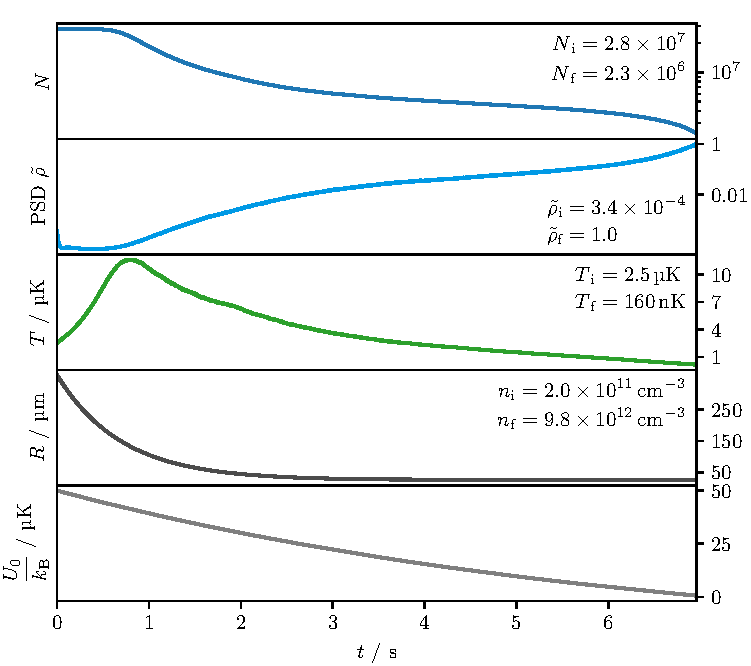
\includegraphics{Evap/Trajectory}
    \caption[Evaporation trajectory for case 5]{It can be seen that the first second does not contribute much to the evaporation. Here, the phase space density \PSD and atom number $N$ are nearly constant while the temperature $T$ increases due to the compression. The atom number and phase space density axes are logarithmic, the others linear.}
    \label{fig:evap_trajectory}
\end{figure}

